\documentclass[11pt,letterpaper,twoside]{article}
\usepackage[tmargin=1in,bmargin=1in,lmargin=1in,rmargin=1in]{geometry}
\usepackage{../style/packages}
\usepackage{../style/commands}
\setbool{notesonly}{false}

% -------------------
% Content
% -------------------
\begin{document}

% Cover Photo
% !TEX root = ../main/aws_chabauty.tex

\thispagestyle{empty}
\newgeometry{
	top=0cm, 
	bottom=0cm, 
	left=0cm, 
	right=0cm
}


\tikz[remember picture,overlay] \node[opacity=1,inner sep=0pt] at (current page.center){
\includegraphics[width=\paperwidth,height=\paperheight]{../cover/swc_poster.jpg}};

\phantom{x} % To image is placed.

% Reset Page Style
\newgeometry{
	top= 1in, 
	bottom= 1in, 
	left= 1in, 
	right= 1in
}
\newpage

% Cover
% !TEX root = ../main/aws_chabauty.tex

\thispagestyle{empty}
\begin{flushright}
\begin{tabular}{ll}
\raisebox{-.5\height}{
\includegraphics[scale=0.055]{../cover/arizona_seal.png}} & {\color{ArzBlue} \Huge University of Arizona} \\
\end{tabular}
\end{flushright}
\vspace{2in}

{%
\color{ArzRed} \Huge \noindent Arizona Winter School 2020 \\[0.2cm] \Huge \color{ArzRed} Nonabelian Chabauty \\[0.2cm] \color{ArzBlue}
\rule{0.70\textwidth}{0.05cm} \vspace{0.1cm}
}

{\color{ArzBlue} \large \noindent Notes By: Caleb McWhorter }

\vfill
\begin{center} {\color{ArzBlue}\huge March 2020} \end{center}
\newpage

% TOC
\thispagestyle{blank}
\tableofcontents
\newpage

% -------------------
% Lectures
% -------------------

% Lecture Notes
\thispagestyle{empty}
\part{Talk Notes} 
    \newpage 
	\setcounter{page}{1}

% Poonen
% !TEX root = ../../../main/aws_chabauty.tex
\newpage
\section{Bjorn Poonen: Introduction to Chabauty's method and Kim's nonabelian generalization}
\subsection{Lecture 1}
\subsubsection{Rational points on Curves}

The starting point is Falting's Theorem, which was originally known as Mordell's conjecture.

\begin{thm}[Falting's, 1983]
Suppose $[K \colon \Q] < \infty$, and let $X$ be a `nice'\footnote{smooth, projective, geometrically integral} curve of genus $g$ over $K$. If $g>1$, then $X(K)$ is finite. 
\end{thm}


There are several proofs now. The first was Falting's proof in 1983 based on Arakelov methods. The next was by Vojta 1991 and its variant (phrased in more elementary terms via Diophantine approximation) by Bomberi. But now there is a proof by Lawrence-Venkatesh in 2018 via $p$-adic period maps. 


For integral points, the parallel to Falting's Theorem is Siegel's Theorem. Let $[K \colon \Q] < \infty$. Let $\O= \O_{K,S}= \{ x \in K \colon \nu(x) \geq 0 \text{ for all } \nu \in S \}$, where $S$ is a finite set of places, including all the archimedean places. Let $U:= X \setminus Z$, where $X$ is a nice curve of genus $g$ and $Z$ is a nonempty 0-dimensional subscheme. Now $\chi(U):= (2-2g) - r$, where $r= \#Z(\overline{K})$ and $\chi(U)$ is the topological Euler characteristic of $U$. Of course, $U$ is a scheme over $K$, so strictly speaking it does not make sense to speak of integral points. In order to talk about integral points, we need to choose a model for $U$ over $\O$, we call this $\cU$. So suppose $\cU$ is a finite type $\O$-scheme with $\cU_K\simeq U$. If $\chi(U)< 0$, then $\cU(\O)$ is finite. The condition that $\chi(U)<0$ is sometimes phrased as `$U$ is hyperbolic' [over $\C$, $\widetilde{U} \simeq b$]. 


\begin{thm}[Siegel's Theorem, 1929]
If $\chi(U)< 0$, then $\cU(\O)$ is finite. 
\end{thm}


There is a proof, obviously, by Siegel. But there are also proofs by Baker-Coates (1970) when either $g \leq 1$ or when $U$ is $y^2= f(x)$ in $\A^2$, and Lawrence-Venkatesh (2018) when $U= \P^1 \setminus \{0,1,\infty\}$. 


\begin{ex}
If $U= \P \setminus \{0,1,\infty\}$ and $\cU= \spec \O[x, \frac{1}{x},\frac{1}{1-x}]$. Then $\cU(\O)$ is the set of solutions to $x+y=1$ with $x,y \in \O^\times$. 
\end{ex}


\begin{rem}
Falting's Theorem is strictly harder than Siegel's Theorem in that Falting's Theorem implies Siegel's Theorem. The key idea is that if $\chi(U)<0$, then there is some finite \etale cover of the affine curve $U$ that is open in a `nice' curve of genus greater than 1. Using descent theory, you can reduce the problem of finding integral points on $U$ to finding integral points on the cover (and perhaps some of its twists). These points will be contained in the rational points, which by Falting's Theorem is a finite set if the genus of the covering curve is sufficiently large. 
\end{rem}


It is natural to ask what happens if we remove the assumption in Siegel's Theorem that $Z$ were nonempty. If $Z$ were empty, then $U= X$, and $X$ is a projective curve. Looking at the integral points on a projective curve, the `valuative' criterion for properness will tell you that the integral points on a projective curve---or anything proper---will be the same as rational points. Then the set that Siegel's Theorem is claiming to be finite would say that the set of rational points on the curve is finite. Then the hyperbolic condition is the same as the condition in Falting's Theorem that $g>1$. Then Siegel's Theorem would specialize to Falting's Theorem in the case where $Z= \emptyset$. Of course, $Z$ needed to be assumed to be nonempty in Siegel's Theorem, so no specialization actually occurs. We can think of this as a Siegel-Falting Theorem. Then in this Siegel-Falting Theorem, the hyperbolic condition $\chi(U)<0$ means that 


\begin{itemize}
\item $g=0$ and $r \geq 3$, or
\item $g=1$ and $r \geq 1$, or
\item $g \geq 2$ and $r$ arbitrary.
\end{itemize}


The problem with nearly all of these methods is that they are not effective.\footnote{The Baker-Coates method is effective.} The goal is then to try to make them effective. This was exactly the hope of Chabauty. 



% Chabauty's Method
\subsubsection{Chabauty's Method}

We will now try to outline what Chabauty did. His method was based on an earlier $p$-adic method by Skolem, who used it to study the unit equation, i.e. the integral point analog. But we shall examine the version for rational points. Let $K/\Q$ be a number field, and let $p$ be a prime with $\p$ be a prime ideal of $K$ lying over $p$.
	\[
	\begin{tikzcd}
	K \arrow[dash,swap]{d}{[K\,:\,\Q]=\,\dim_\Q K} & \p \arrow[dash]{d} \\
	\Q & p 
	\end{tikzcd}
	\]  
Let $X$ be a `nice' curve of genus $g$ over $K$. Let $J= \jac  X$. Now $J$ is a $g$-dimensional abelian variety, so it makes sense to talk about its rational points. Of course, as in Mordell's Theorem,\footnote{Recall that Mordell's Theorem states that the group of $\Q$-rational points on an elliptic curve form a finitely generated abelian group. This was later generalized by Andr\'e Weil and again later by Andr\'e N\'eron to the following: Let $K$ be a field that is finitely generated over its prime field, e.g. any number field, and let $A/K$ be an abelian variety. Then the group of $K$-rational points, denoted $A(K)$, is a finitely generated abelian group. In particular, $A(K) \cong \Z^{r_K} \oplus A(K)_{\text{tors}}$, where $r_K \geq 0$ is the rank and $A(K)_{\text{tors}}$ is the torsion subgroup.} $J$ is a finitely generated abelian group, so it makes sense to talk about the rank of $J$. Define $r= \rank J(K)$. If we were to draw this, it may look something like the following:

	\[
	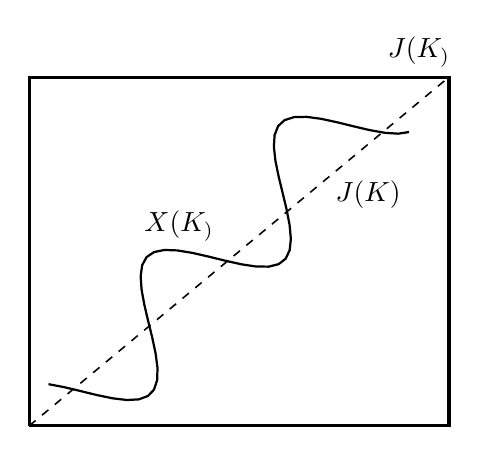
\begin{tikzpicture}
	\begin{axis}[
	hide axis,
	xmin=-3, xmax=6,
	ymin= -2, ymax= 7
	]
	\draw[line width=0.04cm] (-2,-1) -- (5,-1) -- (5,6) -- (-2,6) -- (-2,-1);
	\draw[line width= 0.02cm,dashed] (-2,-1) -- (5,6);
	\addplot[domain=-0.1*pi:2.2*pi, samples=50, black,thick,rotate=45] ({\x+0.5},{-sin(2*\x r)-3});
	\node at (0.5,3) {$X(K_\p)$};
	\node at (4.5,6.5) {$J(K_\p)$};
	\node at (3.65,3.65) {$J(K)$};
	\end{axis}
	\end{tikzpicture}
	\]
where $J(K_\p)$ is the completion of $K$ at $\p$ (a $p$-adic Lie group), the dotted line is the Mordell-Weil group $J(K)$ (a finitely generated abelian group, so a point and all its multiples, which can be dense), and $X(K_\p)$ is the set of local points on the curve (an analytic sub-manifold). The $K$-points of $X$ must lie on both $X(K_\p)$ and $J(K)$. To make this precise, we need an embedding (Abel-Jacobi map). Choose (assuming there is a $K$-rational point at all) $x \in X(K)$ to obtain an Abel-Jacobi map $X \hookrightarrow J$. 
	\[
	\begin{tikzcd}
	X(K) \arrow{r} \arrow{d} &  X(K_\p) \arrow{d} \\
	J(K) \arrow{r} & J(K_\p)
	\end{tikzcd}
	\]
Then the rational points map to rational points, with everything happening in the ambient Lie group $J(K_\p)$. Then we see that the rational points must be in the intersection of the local points $X(K_\p)$ and the Mordell-Weil group $J(K)$. This is the idea. We try to compute this intersection, hoping that the intersection is just the $K$-rational points with nothing `extra'. However in practice, this is difficult. Even writing down equations for $J(K)$ as a projective variety is `bad' enough---nevertheless trying to write down and explicitly work with its group law. So instead, we use the formal logarithm map obtained by integrating 1-forms $p$-adically. 
	\[
	\begin{tikzcd}
	X(K) \arrow{r} \arrow{d} &  X(K_\p) \arrow{d} \\
	J(K) \arrow{r} & J(K_\p) \arrow{r}{\log} & \lie J_{K_\p} \simeq K_\p^g
	\end{tikzcd}
	\]
where $J_{K_\p}$ is the base-change of $J(K)$ to the local field $K_\p$, i.e. an abelian variety defined over $K_\p$. Under this map, we transform the group law into addition in a vector space, which is much simpler to work with. So rather than trying to find the intersection of $X(K_\p)$ and $J(K)$ in $J(K_\p)$, we push everything `foward' and try to compute them in the vector space $K_\p^g$. [Notice the torsion subgroup `dies' because there is clearly no torsion in $K_\p^g$.]


Let's say a bit more about the log map. The log map is `close' to being an isomorphism. The kernel of the log map is finite (in fact, it is the torsion subgroup of $J(K_\p)$) and is a local diffeomorphism. Then the image of the log map will be open and compact ($J$ is a compact) subgroup of the $p$-adic vector space $K_\p^g$. [It is not necessarily an $\O_\p$-module, but it is a $\Z_\p$-module of full rank.] Therefore, the image of log is an open compact subgroup of the Lie group $\lie J_{K_\p}$. Moreover, the image of $J(K) \to K_\p^g$ is generated by $r$ elements, namely the generators of $J(K)$. Then the dimension of the $K_\p$-span of the image of the map $J(K) \to K_\p^g$ is at most $r$.


If $r< g$, there exists a nonzero linear functional $\lambda: \lie J_{K_\p} \to K_\p$ vanishing on $\im J(K)$, and $\lambda$ pulls back to a nonzero locally analytic function on $X(K_\p)$ vanishing on $X(K)$. Because on each residue disk $\lambda$ is a nonzero power series in a one-dimensional space, it has at most finitely many zeros on each closed disk (in this compact space). Therefore, $X(K)$ itself is finite. But of course, this all requires what might be called Chabauty's condition: $r<g$. If this condition fails, then the dotted points in our diagram could be dense, which would make it extremely difficult to find where they intersect the curve. 


Obviously, the difficulty in all of this is working with the Jacobian, which can be unwieldy. How do we limit the role of the Jacobian in this method? This idea was Kim's generalization. But before discussing that, let's see how we can restate this method while avoiding the use of Jacobians---the first step Kim had to take in his generalization. We begin with the same diagram as before, but now we $p$-adically complete the groups $J(K)$ and $J(K_\p)$, and invert $p$ in each. 
	\[
	\begin{tikzcd}
	X(K) \arrow{d} \arrow{r} & X(K_\p) \arrow{d} \\
	J(K) \arrow{r} \arrow{d} & J(K_\p) \arrow{r}{\log} \arrow{d} & \lie J_{K_\p} \\
	\widehat{J(K)}[\frac{1}{p}] & \widehat{J(K_\p)}[\frac{1}{p}] 
	\end{tikzcd}
	\]
Before continuing, we should remind the reader of $p$-adic completion. Given an abelian group $M$, we want to turn $M$ into a $\Z_p$-module. Define the $p$-adic completion to be $\hat{M}:= \plim M/p^nM$, which is a $\Z_p$-module. But of course, this is not a field. So we change this from $\Z_p$ to $\Q_p$ by localizing, i.e. inverting $p$. This is $\hat{M}[\frac{1}{p}] \simeq \hat{M} \otimes_{\Z_p} \Q_p$, which is a $\Q_p$ vector space. Now completion and localizing are functors, so we obtain a map $\widehat{J(K)}[\frac{1}{p}] \to \widehat{J(K_\p)}[\frac{1}{p}]$. From the discussion above, we knew that $\log$ was a local diffeomorphism. The only thing `getting in the way' of it being an isomorphism was torsion. But $\widehat{J(K_\p)}[\frac{1}{p}]$ is a $\Q_p$-vector space---there's no torsion left! This gives us the following diagram
	\[
	\begin{tikzcd}
	X(K) \arrow{d} \arrow{r} & X(K_\p) \arrow{d} \\
	J(K) \arrow{r} \arrow{d} & J(K_\p) \arrow{r}{\log} \arrow{d} & \lie J_{K_\p} \\
	\widehat{J(K)}[\frac{1}{p}] \arrow{r} & \widehat{J(K_\p)}[\frac{1}{p}] \arrow{ur}{\rotatebox{45}{$\sim$}} 
	\end{tikzcd}
	\]
 

The next step is to re-express everything in terms of \etale homology. In 2-descent for elliptic curves, we look at the map $E(K)/2E(K) \to H^1(K,E[2])$, i.e. the Kummer map. Everything we have is built from quotients that behave like this, e.g. $J(K)/pJ(K)$. So there should be a analogous descent into some Galois cohomology. This something is the cohomology of the Galois group of $K$ acting on some kind of Tate module, which we will write $H^1(K,V)$, and its local version $H^1(K_\p,V)$. But what is $V$? We can think of $V$ as some kind of \etale homology.\footnote{See David Corwin's notes \href{https://math.berkeley.edu/~dcorwin/files/ChabautytoKim.pdf}{From Chabauty's method to Kim's non-abelian Chabauty method}} 


As a motivation, if $X$ is a curve over $\C$ and $J$ is its Jacobian, then analytically as a complex manifold, $J(\C) \simeq \C^g/ \Lambda$, where $\Lambda$ is a rank $2g$ lattice. But $\Lambda$ is also the fundamental group of the space, easily seen from the fact that the universal cover is $\C^g$. Then we can view $\Lambda$ as the homology $\Lambda= H_1(J(\C),\Z)$. Of course, viewing $J(\C)$ as $\C^g/\Lambda$ is far simpler because the group law has been turned into `traditional' addition. Viewing $J(\C)$ as $\C^g/\Lambda$, it is easy to see that 
	\[
	J[p] \simeq \frac{1}{p} \Lambda/\Lambda \ma{\stackrel{p}{\sim}} \Lambda/p\Lambda= H_1(J(\C), \Z/p\Z)= H_1(X(\C),\Z/p\Z) 
	\]
where we have used the homology groups, $H_1$, for curves and their Jacobians are the same. But now there is no $J$ involved! So we can talk about the $p$-torsion of the Jacobian without actually involving $J$. This can be done similarly for the $p^n$-torsion, and so on. 


We want to create an analog of this for a curve that is not over the complex numbers. But if we are not using $\C$, we are going to have to switch to \Etale (co)homology. For $X$ over $K$, $J[p] \simeq H_1^\et(X_{\ov{K}}, \Z/p\Z):= \Z/p\Z$-dual of $H^1_\et(X_{\ov{K}}, \Z/p\Z)$. [Note, one should only take \etale (co)homology of a geometric object, so be sure to base change to an algebraic closure first.] Similarly, $J[p^n] \simeq H_1^\et(X_{\ov{K}}, \Z/p^n\Z)$. Now taking inverse limits, we obtain the $\Z_p$ Tate module $T:= \plim J[p^n] \simeq H_1^\et(X_{\ov{K}}, \Z_p)$. Again to avoid rings that are not fields, tensoring with $\Q_p$, we obtain the $\Q_p$ Tate module $V:= T[\frac{1}{p}]= T \otimes_{\Z_p} \Q_p \simeq H_1^\et(X_{\ov{K}}, \Q_p)$ obtained by inverting $p$, which is a $\Q_p$-vector space of dimension $2g$. There is always a way of moving from a vector space to an algebraic group whose points are the vector space. Because it will later be useful to think of $V$ in this way, write $\cV(\Q_p)$ for a group variety $\cV \simeq \G_a^{2g}$, the group variety over $\Q_p$. As a variety, $\cV$ is $\A^{2g}$ with an additive group law (coordinate-wise addition). The group $G_K:= \Gal(\ov{K}/K)$ acts continuously on all of these, e.g. $G_K \to \Aut \cV \simeq \GL_n(\Q_p)$, as a group variety. 


% !TEX root = ../../../main/aws_chabauty.tex
\newpage
\subsection{Lecture 2}
\subsubsection{Selmer Groups}

Last time, we had the following diagram which we wanted to rephrase in terms of something without Jacobians.
	\[
	\begin{tikzcd}
	X(K) \arrow{d} \arrow{r} & X(K_\p) \arrow{d} \\
	J(K) \arrow{r} \arrow{d} & J(K_\p) \arrow{r}{\log} \arrow{d} & \lie J_{K_\p} \\
	\widehat{J(K)}[\frac{1}{p}] \arrow{r} & \widehat{J(K_\p)}[\frac{1}{p}] \arrow{ur}{\rotatebox{45}{$\sim$}} 
	\end{tikzcd}
	\]
To begin, we defined a $\Qp$ Tate module, which we called $V$, defined in terms of the \etale homology of the curve. Now we want to relate the rational points to these Galois cohomology groups using Selmer groups and the descent map. 


We begin with the Kummer sequence for this Jacobian
	\[
	0 \ma{} J[p] \ma{} J \ma{p} J \ma{} 0
	\]
Now taking Galois cohomology yields
	\[
	J(K) \ma{p} J(K) \ma{} H^1(K, J[p])
	\]
We can contract this as
	\[
	\dfrac{J(K)}{pJ(K)} \hookrightarrow H^1(K,J[p])
	\]
Originally, this was done to prove the Mordell-Weil theorem by bounding $J(K)/pJ(K)$, which was the first step in proving that $J(K)$ is finitely generated. It would be nice if $H^1(K,J[p])$ were finite; however, $H^1(K,J[p])$ is an infinite dimensional $\F_p$-vector space if $\dim J \geq 0$. But perhaps, studying the image of this inclusion more carefully, it can be shown that there is some finite subspace of $H^1(K,J[p])$ which bounds $J(K)/pJ(K)$, or at least figure out which of the classes in $H^1(K,J[p])$ come from $J(K)/pJ(K)$. The idea will be not to look at what is in the image directly but rather look what is in the image locally. So using functoriality, we can write down the following commutative diagram  
	\[
	\begin{tikzcd}
	\dfrac{J(K)}{pJ(K)} \arrow[hook]{r} \arrow{d} & H^1(K,J[p]) \arrow{d} \\
	\dfrac{J(K_\nu)}{pJ(K_\nu)} \arrow[hook]{r} & H^1(K_\nu,J[p])
	\end{tikzcd}
	\]
For a class in $H^1(K,J[p])$ to have come from $J(K)/pJ(K)$, it must appear in the inclusion into $H^1(K_\nu,J[p])$ by following the commutativity of the diagram. So we have a condition for classes from $J(K)/pJ(K)$ to appear in $H^1(K,J[p])$. Of course, we can do this for all $\nu$, in which case we obtain the following diagram, which will give us the Selmer group.
	\[
	\begin{tikzcd}
	\dfrac{J(K)}{pJ(K)} \arrow[hook]{r} \arrow{d} & H^1(K,J[p]) \arrow{d} \\
	\prod_\nu \dfrac{J(K_\nu)}{pJ(K_\nu)} \arrow[hook]{r} & \prod_\nu H^1(K_\nu,J[p])
	\end{tikzcd}
	\]
The $p$-Selmer group, which is a subgroup of the global Galois cohomology $H^1(K,J[p])$ which contains the image of the inclusion $J(K)/pJ(K) \hra H^1(K,J[p])$.
	\[
	\begin{tikzcd}
	\dfrac{J(K)}{pJ(K)} \arrow[hook]{r} \arrow{d} & \sel_p J \arrow[draw=none]{r}[sloped,auto=false]{\subseteq} & H^1(K,J[p]) \arrow{d}{\beta} \\
	\prod_\nu \dfrac{J(K_\nu)}{pJ(K_\nu)} \arrow[hook]{rr}{\alpha} & & \prod_\nu H^1(K_\nu,J[p])
	\end{tikzcd}
	\]


\begin{dfn}[$p$-Selmer group]
The $p$-Selmer group, denoted $\sel_p J$, is $\{ \xi \in H^1(K,J[p]) \colon \beta(\xi) \in \im \alpha \}$. 
\end{dfn}


\begin{rem}
This group is finite and computable. Moreover, this gives the only currently known way of bounding ranks of abelian varieties over number fields. Other arguments reduce to this method in some way. 
\end{rem}


We can repeat this same argument using powers of $p$.
	\[
	\dfrac{J(K)}{p^nJ(K)} \hookrightarrow \sel_{p^n} J \subset H^1(K,J[p^n])
	\]
By taking inverse limits, we obtain the $p$-adic completion of the Mordell-Weil group.\footnote{In Iwasawa Theory, direct limits are taken instead of inverse limits.}
	\[
	\hat{J(K)} \hookrightarrow \sel_{\Z_p} J \subset H^1(K,T)
	\]
where $T$ is the Tate module. Again to avoid rings which are not fields, we invert $p$ to obtain
	\[
	\hat{J(K)}\left[\frac{1}{p}\right] \hookrightarrow \sel_{\Qp} J \subset H^1(K,V)
	\]
The Selmer groups are acting as upper bounds for the Jacobians. But we want to say more about the `error' in the approximation. The obstruction, or error, here is the Shafarevich-Tate group, $\sha$. Classically, we have the group which we are trying to compute, $J(K)$, the `approximation' $\sel_p J$, and the `error' $\sha[p]$.
	\[
	0 \ma{} \dfrac{J(K)}{pJ(K)} \ma{} \sel_p J \ma{} \sha[p] \ma{} 0
	\]
Proceeding just as we did above, i.e. taking inverse limits and inverting $p$, we obtain
	\[
	0 \ma{} \hat{J(K)}\left[\frac{1}{p}\right] \ma{} \sel_{\Qp} J \ma{} \left( \plim \sha[p^n] \right)\left[\frac{1}{p}\right] \ma{} 0
	\] 
The group $\sha$ is conjecturally finite. But then, conjecturally, the groups $\sha[p^n]$ stabilize for sufficiently large $n$. The maps in $\left( \plim \sha[p^n] \right)\left[\frac{1}{p}\right]$ are multiplication by $p$. So the term $\left( \plim \sha[p^n] \right)\left[\frac{1}{p}\right]$ is conjecturally zero if $\sha[p^n]$ is finite. But then $\hat{J(K)}\left[\frac{1}{p}\right]$ is a $\Qp$-vector space of dimension equal to the rank, exactly approximated by $\sel_{\Qp} J$. 


Notice we still have not succeeded in completely eliminating Jacobians. However, we have made some progress in our original diagram by injecting Selmer groups. 
	\[
	\begin{tikzcd}
	X(K) \arrow{d} \arrow{r} & X(K_\p) \arrow{d} \\
	J(K) \arrow{r} \arrow{d} & J(K_\p) \arrow{r}{\log} \arrow{d} & \lie J_{K_\p} \\
	\widehat{J(K)}[\frac{1}{p}] \arrow{r} \arrow{d} & \widehat{J(K_\p)}[\frac{1}{p}] \arrow{ur}{\rotatebox{45}{$\sim$}} \\
	\sel_{\Qp} J \arrow{d} \\
	H^1(K,V) \arrow{r} & H^1(K_\p,V)
	\end{tikzcd}
	\]
The next step will be to find a way of describing the Selmer group $\sel_{\Qp} J$ that does not involve $J$.



% Bloch-Kato Selmer Groups
\subsubsection{Bloch-Kato Selmer Group}

We want to describe $\sel_{\Qp}$ solely in terms of $V$ and not $J$. Rather than immediately discuss the $V$ we had talked about before, we will speak in the more general setting of local Galois representations. Let $V$ be a finite dimensional $\Qp$-vector space with continuous $G_{K_\nu}$-action, where $G_{K_\nu}:= \Gal(\overline{K}_\nu/K_\nu)$. We first define an important object created by Fontaine
	\[
	D_{\cris}(V):= (B_{\cris} \otimes_{\Qp} V)^{G_{K_\nu}}
	\]
where $B_{\cris}$ is a certain ring equipped with a $G_{K_\nu}$-action. We will not worry ourselves precisely what this is, which requires a discuss (at the very least) of Witt vectors. Now it is a fact that $\dim_{K_\nu} D_{\cris}(V) \leq \dim_{\Qp} V$. We say that $V$ is crystalline if, in fact, equality holds. 


To get an idea of what this condition is, fix a $\nu$ and consider an abelian variety $J/K_\nu$, then $J$ has good reduction if and only if its $\Qp$ Tate module $V$ is unramified (if $\nu \nmid p$) or crystalline (if $\nu \mid p$). We will need one other definition, so suppose $\xi \in H^1(K,V)$. The cohomology class is naturally associated to an extension of $\Qp$ by $V$, namely\footnote{Note that $E$ here has nothing to do with elliptic curves\dots it is just the first letter of the word extension.}
	\[
	0 \ma{} V \ma{} E \ma{} \Qp \ma{} 0
	\]
What is the correspondence? These are all local Galois representations. Now $\Qp$ has a trivial action. Given $\xi$, we can write down a vector space $E$ with the extensions given as above. Going the other way, given the extension as above, we take the element of $H^0(K_\nu,\Qp)$ from $\Qp$, namely 1. This element will map to $H^1(K_\nu,V)$, which will be our $\xi$. In any case, let the sequence above be the corresponding extension. We call $\xi$ crystalline if $E$ is crystalline (because $E$ is a local Galois representation). We could define $\xi$ to be crystalline if it is in the kernel of the map from $H^1(K_\nu,V)$ to $H^1(K_\nu, B_\cris \otimes V)$. We now can define a subset of all the crystalline cohomology classes, as Block-Kato did. So define $H_f^1(K_\nu,V):= \{ \text{crystalline classes in } H^1(K_\nu,V) \}$. 


\begin{rem}
Suppose that $\p \mid p$. If $J$ is an abelian variety with good reduction at $\p$, and $V$ is a $\Qp$ Tate module, then the image of the Kummer descent map $\hat{J(K_\p)}[\frac{1}{p}] \to H^1(K_\p,V)$ is $H_f^1(K_\p,V)$. [If $\p \nmid p$, then $H^1(K_\p,V)= 0$.] This is a generalization of the fact that for elliptic curves, if you look at a prime of good reduction and you look at the image of the local  points inside the local Galois cohomology, you obtain exactly the unramified classes. In our case here, we obtain the crystalline classes. 
\end{rem}



% Global Galois Representations
\subsubsection{Global Galois Representations}

We now have a way of talking about local points without referring to the Jacobian anymore. Namely, the image of the local points of the Jacobian can be characterized just in terms of $V$ by using crystalline cohomology classes. We need to do this globally, rather than just locally. Let $V$ be a finite dimensional $\Qp$-vector space with continuous $G_K$-action. Given a global cohomology class $\xi \in H^1(K,V)$, we can obtain a local cohomology class $\xi_\nu$, namely the image of $\xi$ in $H^1(K_\nu,V)$. We define the Bloch-Kato Selmer group of $v$ to be the group $H_f^1(K,V):= \{ \xi \in H^1(K,V) \colon \xi_\nu \text{ is crystalline for all } \nu \mid p \}$, i.e. the set of global cohomology classes satisfying the local conditions. 


We can now re-express the Selmer group in Bloch-Kato terms, without referring to $J$. If $J$ is an abelian variety over $K$ and $V$ is a $\Qp$ Tate module, then the Bloch-Kato Selmer group is $H_f^1(K,V)= \sel_{\Qp} J$, which is just the classical $\Qp$ Selmer group of $J$. Now we can talk about the Selmer group $\sel_{\Qp} J$ using $H_f^1(K,V)$, which depends only on $X$ because $V$ depends only on $X$. We can now return to our diagram and fill in even more by replacing $\sel_{\Qp} J$ with $H_f^1(K,V)$, mapping $\widehat{J(K_\p)}[\frac{1}{p}]$ to $H_f^1(K_\p,V)$, which are subgroups of $H^1(K,V)$ and $H^1(K_\p,V)$, respectively. We have the restriction map $H_f^1(K,V) \to H_f^1(K_\p,V)$ and local coboundary map $\widehat{J(K_\p)}[\frac{1}{p}] \to H_f^1(K_\p,V)$. This gives us the following diagram
	\[
	\begin{tikzcd}
	X(K) \arrow{d} \arrow{r} & X(K_\p) \arrow{d} \\
	J(K) \arrow{r} \arrow{d} & J(K_\p) \arrow{r}{\log} \arrow{d} & \lie J_{K_\p} \\
	\widehat{J(K)}[\frac{1}{p}] \arrow{r} \arrow{d} & \widehat{J(K_\p)}[\frac{1}{p}] \arrow{ur}{\rotatebox{45}{$\sim$}} \arrow{d} \\
	\sel_{\Qp} J \arrow{d}= H_f^1(K,V) \arrow{r} &  H_f^1(K_\p,V) \arrow{d} \\
	H^1(K,V) \arrow{r} & H^1(K_\p,V)
	\end{tikzcd}
	\]














% 31:46

The only thing left to do is remove the tangent space at the identity, $\lie J_{K_\p}$. For this, we will need one more definition. 


Algebraic de Rham Cohomology: $H_\dr^1(X):= \H^1(X,\Omega^0)$ with Hodge filtration $\Fil^0$, where $\H$ is hypercohomology. Define also $H_1^\dr(X):=$ dual of $H_\dr^1$ with dual filtration. 


	\[
	\begin{tikzcd}
	X(K) \arrow{d} \arrow{r} & X(K_\p) \arrow{d} \\
	J(K) \arrow{r} \arrow{d} & J(K_\p) \arrow{r}{\log} \arrow{d} & \lie J_{K_\p} \\
	\widehat{J(K)}[\frac{1}{p}] \arrow{r} \arrow{d} & \widehat{J(K_\p)}[\frac{1}{p}] \arrow{ur}{\rotatebox{45}{$\sim$}} \arrow{d} \\
	\sel_{\Qp} J \arrow{d}= H_f^1(K,V) \arrow{r} &  H_f^1(K_\p,V) \arrow{d} \arrow{r}{\log, \sim} &  H_1^\dr(K_{K_\p})/\Fil^0 \\
	H^1(K,V) \arrow{r} & H^1(K_\p,V)
	\end{tikzcd}
	\]


We get 
	\[
	\begin{tikzcd}
	X(K) \arrow{r} \arrow{d} & X(K_\p) \arrow{d} \arrow{dr}{p\text{-adic integrals}} \\
	H_f^1(K,V) \arrow{r} &  H_f^1(K_\p,V) \arrow{r}{\sim} & H_1^\dr(X_{K_\p})/\Fil^0
	\end{tikzcd}
	\]



% Lower Central Series
\subsubsection{Lower Central Series}

Let $G$ be a (topological) group. For $A, B \leq g$, define $(A,B):= \ov{\langle aba^{-1}b^{-1} \colon a \in A, b \in B \rangle}$. Now define the lower central series by
	\[
	\begin{aligned}
	C^1G&:= G \\
	C^2G&:= (G,C^1G)= (G,G) \\
	C^3G&:= (G,C^2G) \\
	&\phantom{=}\vdots
	\end{aligned}
	\]
Finally, define $G_n:= G/C^{n+1}G$. This is a $n$-step nilpotent group. 


\begin{ex}
$G_1= G/(G,G)=: G^{\ab}$, the abelianization of $G$, i.e. the largest abelian quotient. 
\end{ex}


This was just Group Theory. Now let's apply this to the fundamental group of the curve.



% Abelianized Fundamental Group
\subsubsection{Abelianized Fundamental Group}

Given $M$ a connected real manifold, $m \in M$, we get $\pi_1(M,m)^\ab \simeq H_1(M,\Z)$, where $\pi_1$ is the fundamental group. What is the algebraic version? Given $X$, a `nice' curve of genus $g$ curve over $K$, $x \in X(K)$, we obtain
	\[
	\pi_1^\et(X_{\ov{K}}, x)^\ab \simeq H_1^\et(X_{\ov{K}}, \hat{\Z})
	\]
But we have maps
	\[
	\pi_1^\et(X_{\ov{K}},x)_1 \ma{\sim} \pi_1^\et(X_{\ov{K}}, x)^\ab \simeq H_1^\et(X_{\ov{K}}, \hat{\Z}) \sra H_1^\et(X_{\ov{K}}, \Z_p) \subset H_1^\et(X_{\ov{K}}, \Qp)=: V= \cV(\Qp)
	\]


Kim obtains a generalization
	\[
	\pi_1^\et(X_{\ov{K}},x) \ma{} V_n= \cV_n(\Qp)
	\]
where $\cV_n$ is some unipotent algebraic group, and
	\[
	\begin{tikzcd}
	X(K) \arrow{d} \arrow{r} & X(K_\p) \arrow{d} \arrow{dr}{p\text{-adic iterated integrals}} \\
	H_f^1(K,V_n) \arrow{r} & H_f^1(K_\p,V_n) \arrow{r}{\sim} & \pi_1^\dr(X_{K_\p},x)_n/\Fil^0
	\end{tikzcd}
	\]
and morphisms of $\Qp$-varieties
	\[
	\sel^{[n]} \ma{} J^{[n]} \ma{} L^{[n]}
	\]
which gives you the $\Qp$ points of $\pi_1^\dr(X_{K_\p},x)_n/\Fil^0$. 


\begin{thm}[Kim]
If for some $n \geq 1$, $\dim \sel^{[n]} < \dim J^{[n]}$, then $X(K)$ is contained in the set of zeros of some nonzero locally analytic functions on the local points of the curve, which are given by some iterated integrals. Therefore, $X(K)$ is finite.
\end{thm}

















% Balakrishnan
% !TEX root = ../../../main/aws_chabauty.tex
\newpage
\section{Jennifer Balakrishnan: Computational tools for quadratic Chabauty}
\subsection{Lecture 1}

\begin{ques}
Does there exist a pair of rational right triangles and a rational isoceles triangle that have the same area and the same perimeter?
\end{ques}

	\begin{figure}[!ht]
	\centering
	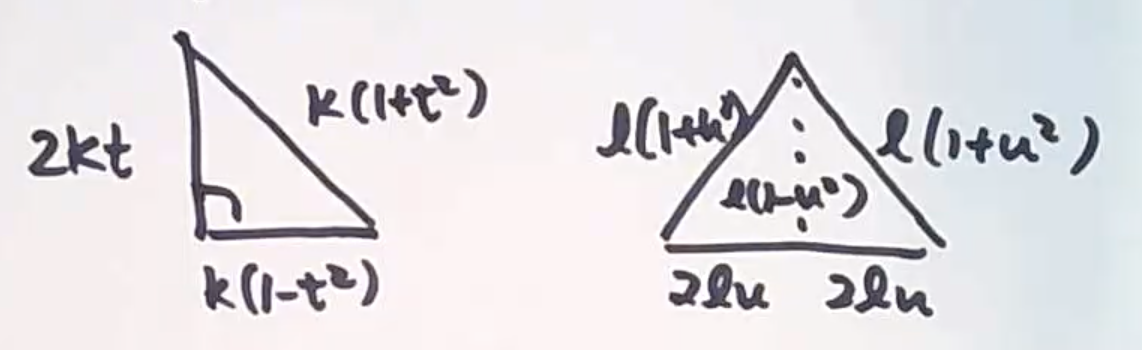
\includegraphics[width=0.6\textwidth]{../images/im4.png}
	\end{figure}


We rescale $l=1$, suppose $k,t,u \in \Q$, $0<t,u<1$, $k>0$


Equate areas and perimeters:
	\[
	\begin{cases}
	k^2t(1-t^2)= 2u(1-u^2) \\
	k+kt= 1+2u+u^2
	\end{cases}
	\]


After some algebra, we see there exists $x \in \Q$, $1<x<2$ such that $2xk^2+(-3x^2-2x^2+6x-4)k+x^5= 0$. The discriminant of polynomial in $k$ must be a rational square:
	\[
	\begin{aligned}
	y^2&= (-3x^2-2x^2+6x-4)^2-4(2x)x^5 \\
	&=x^6+12x^5-32x^4+52x^2-48x+16
	\end{aligned}
	\]
This is a genus 2 curve, and we'd like to determine $X(\Q)$. The Jacobian $J$ of $X$ has rank $\rank J(\Q)=1$. Also, Chabauty-Coleman bound gives $\#X(\Q) \leq 10$. We can find 
	\[
	\{\infty^\pm, (0,\pm 4), (1,\pm 1), (2, \pm 8), (12/11,\pm 868/11^3) \} \subseteq X(\Q)
	\]
We've found no rational points!


The answer to the discriminant question:


\begin{thm}[Hirakawa-Matsumura, 2018]
Yes, there are exactly one pair of such triangles.
\end{thm}



% Coleman's Effective Chabauty
\subsubsection{Coleman's Effective Chabauty}

Let $X/\Q$ be a `nice' curve with genus $g \geq 2$. Suppose that $\rank J(\Q)< g$. If $p>2g$ is good, then $\#X(\Q) \leq \#X(\F_p) + 2g - 2$. This bound comes from bounding the number of zeros of a $p$-adic (Coleman) integral.


Coleman gave a theory of $p$-adic line integration in the 1980s. 


\begin{thm}[Coleman]
Let $X/\Q_p$ be a nice curve with good reduction at $p$. The $p$-adic itnegral $\int_P^Q \omega \in \ov{\Q}_p$, defined for $P,Q \in X(\ov{\Q}_p)$ and $\omega \in H^0(X,\Omega^1)$ satisfies the following:

\begin{enumerate}[(i)]
\item the integral is $\ov{\Q}_p$ linear in $\omega$
\item if $P,Q$ reduce to the same point $\ov{P} \in X(\ov{\F}_p)$, then we call the integral a `tiny' integral.
\item We have
	\[
	\int_P^Q \omega + \int_{P'}^{Q'} \omega= \int_P^Q \omega + \int_{P'}^Q \omega
	\]
then we can define $\int_D^\omega$ for $D= \sum_{j=1}^n ((Q_j)-(P+j)) \in DN_K^0(\ov{\Q}_p)$ as $\int_P \omega= \sum_{j=1}^n \int_{P_j}^{Q_j} \omega$.
\item if $D$ is principal, then $\int_D \omega= 0$.
\item Integral compatibility with $\Gal(\ov{\Q}_p/\Q_p)$-action.
\item Fix $P_0 \in X(\ov{\Q}_p)$. If $0 \neq \omega \in H^0(?,\Omega^1)$, then the set of points $P \in X(\ov{\Q}_p)$ reduces to a fixed point on $X(\F_p)$ such that $\int_{P_0}^{P_1} \omega= 0$ is finite. 
\end{enumerate}
\end{thm}


This is the Coleman integral. Cont Given hypotheses of previous theorem, let $b \in X(\Q_p)$, $i: X \hra J$ given by $P \mapsto [P-b]$. There is a map $J(\Q_p) \times H^0(X_{\Q_p},\Omega^1) \to \Q_p$ given by $(Q,\omega) \mapsto \langle Q,\omega \rangle$ that's additive in $Q$, $\Q_p$-linear in $\omega$, and given by $\langle [D],\omega \rangle= \int_D \omega$ for $D \in \div_X^0$.


For $P \in X(\Q_p)$, we have the Abel-Jacobi morphism $Aj_b$ that takes $P$ to 
	\[
	\langle i(P), \omega \rangle= \int_b^P \omega =: AJ_b(P)
	\]
The Chabauty-Coleman method uses a certain subspace of the space of regular 1-forms. Now assume $b \in X(\Q)$, use it to embed $X \hra J$.


\begin{dfn}
Let $A= \{ \omega \in H^0(X,\Omega^1) \text{ for all } P \in J(\Q), \langle P,\omega \rangle=0 \}$ be the subspace of annihilating differentials.  
\end{dfn}


We have
	\[
	\begin{tikzcd}
	X(\Q) \arrow{d} \arrow{r} & X(\Q_p) \arrow{d} \arrow{dr}{AJ_b} \\
	J(\Q) \arrow{r} & J(\Q_p) \arrow{r}{\log} &  H^0(J_{\Q_p},\Omega^1) \simeq H^0(X_{\Q_p}, \Omega^1)
	\end{tikzcd}
	\]
By ``computing rational points via Chabauty-Coleman: compute the finite set of $p$-adic points
	\[
	X(\Q_p)_1:= \{ z \in X(\Q_p) \colon \int_b^z \omega= 0 \text{ for all } \omega \in A \}
	\]
By construction, $X(\Q) \subset X(\Q_p)$. How do we compute annihilating differ?


\begin{ex}
Let $X: y^2= x^5-2x^3+x=1$ (LMFBD: 971.4 971.1) Some facts about $X$:
\begin{enumerate}[(i)]
\item $X(\Q)_{\text{known}}= \{ \infty, (0,\pm1/2), (-1,\pm1/2), (1,\pm 1/2)\}$
\item $J$ is simple, $J(\Q) \simeq \Z$, $[(-1,-1/2)-(0,1/2)] \in J(\Q)$ has infinite order.
\item $X$ is good at $p=3$, $\#X(\F_3)=7$. Stoll's refinement of Chabauty-Coleman for $p= 3$:
	\[
	\#X(\Q) \leq \#X(\F_p) + 2 r + \dfrac{2r}{p-2}= 11
	\]
\end{enumerate}
So need to do more work to determine $X(\Q)$ here. We will construct a 3-adic annihilating differential $\eta$. Basts of $H^0(X_{\Q_p},\Omega^1)$ is $\left\{ \omega_i = \dfrac{x^i \;dx}{2y} \right\}_{i=0,1}$. So $\eta$ is a $\Q_3$-linear combination of $\omega_0, \omega$. We will compute the values of $\alpha;= \int_{(a,b)}^{1-\gamma_0} \omega_0$ and $\beta:= \int_{(0,\gamma_0)}^{1-\gamma_0} \omega$ to compute $\eta$. SageMath can compute $\alpha, \beta$
	\[
	\begin{aligned}
	\alpha&= 3+3^2+3^4+\cdots \\
	\beta&= 2 + 2\cdot 3 + 2 \cdot 3^2 + \cdots
	\end{aligned}
	\]
We take $\eta= \beta \omega_0 - \alpha \omega_1$ and run Chabauty-Coleman. 
\end{ex}


Where do these numbers come from?



% Explicit Coleman Integration
\subsubsection{Explicit Coleman Integration}

Using the action of Frobenius on $p$-adic cohomology. (Sage for hyperelliptic curves or Magma for plane curves.) Let $X^\an$ denote the rigid analytic space over $\Q_p$ associated to $X/\Qp$. A wide open subspace of $X^\an$, the complement in $X^\an$ of the union of a finite collection of disjoint closed disks of radius $<1$. Now for some more properties of the Coleman integral:

\begin{thm}[Coleman]
Let $\eta, \xi$ be 1-forms on a wide open $V$ of $X^\an$, $P,Q, R \in V(\ov{\Qp})$, let $a,b \in \ov{\Qp}$. Then we have 
\begin{enumerate}[(i)]
\item linearity in integrand:
	\[
	\int_P^Q a\eta + b \xi= a \int_P^Q \eta + b \int_P^Q \xi
	\]
\item additivity in endpoints
	\[
	\int_P^R \eta + \int_R^Q \eta= \int_P^Q \eta
	\]
\item change of variables under rigid analytic maps (Frobenius)
\item Fundamental Theorem of Calculus
	\[
	\int_P^Q df= f(P) - f(Q)
	\]
\item Galois compatability
\end{enumerate}
\end{thm}


We first integrate $\int_P^Q \omega$ for $\omega$ 1-form of the second kind, $P, Q \in V(\Qp)$. Suppose $X$ is a hyperelliptic curve. Sketch of explicit Coleman integration (B-Bradshaw-Kedlaya).


\begin{enumerate}[1.]
\item take a lift of $p$-power Frobenius
\item compute a basis $\{ \omega_i \}$ of 1-forms of the second kind
\item compute $\phi^* \omega_i$ via Kedlaya's zeta function algorithm and use properties of Coleman integral to relate
	\[
	\int_P^Q \phi^*\omega_i \text{ to } \int_P^Q \omega_i
	\]
as well as other easier terms.
\item solve for $\int_P^Q \omega_i$ using lth. algorithm.
\end{enumerate}
 

We sketch Kedlaya's algorithm. Let $X$ be the curve $y^2= p(x)$. We work in an affine $Y \subset X$ given by defining Weierstrass points. Take $\phi$ to be $x \mapsto x^p$ and $y \mapsto y^p \sum_{j=0}^\infty \binom{1/2}{1} \left( \dfrac{p(x^p - p(x)^p}{y^{2p}} \right)^j$. Then we compute the action of $\phi$ on
	\[
	\begin{aligned}
	\phi^*\left( \dfrac{x^i \;dx}{y} \right)&= \dfrac{x^{pi} \;d(x^p)}{\phi(y)} \\
	&= \dfrac{x^{pi} p x^{p-1} \;dx}{\phi(y)} \\
	&= p x^{pi + p - 1} y^{-p} \sum_{j=0}^\infty \binom{1/2}{1} \left( \dfrac{p(x^p - p(x)^p}{y^{2p}} \right)^j
	\end{aligned}
	\]
and reduce pole order of each resulting differential using relations in $H^1$. Denote the basis by $\{\omega_i\}_{i=0,\ldots,2g-1}$. Then Kedlaya's algorithm gives
	\[
	\phi^* \omega_i= dh_o + \sum_{j=0}^{2g-1} \mu_{ji} \omega_j
	\]
If we can compute $h_i$ and $M$, then
	\[
	\begin{pmatrix}
	\vdots \\
	\int_P^Q \omega_i \\
	\vdots
	\end{pmatrix}=
	(M^t - I)^{-1} 
	\begin{pmatrix}
	\vdots \\
	h_i(P) - h_i(Q) - \int_P^{\pi(P)} \omega_i - \int_{\phi(Q)}^Q \omega_i \\
	\vdots
	\end{pmatrix}
	\] % *


Finishing the 3-adic integrals on $y^2= x^5 - 2x^3 + x + 1/4$, we constructed $\eta= \beta \omega_0 - \alpha \omega_1$, where $\alpha,\beta$ are computed using (*). We want to compute $X(\Q_3)$. Compute power series expansions of
	\[
	\left\{ \int_{(0,1/2)}^{P_t} \eta \right\}
	\]
where $P_t$ ranges over all residue disks:
	\[
	\int_{(0,1/2)}^{P_t} \eta= \underbrace{\int_{(0,1/2)}^{P_0} \eta}_{\text{Gives 3-adic}} + \underbrace{\int_{P_0}^{P_t} \eta}_{\text{Coleman 3-adic series}}
	\]
Lucky fact: For each residue disk, there exists $P_0 \in X(\Q)$, the 3-adic number is 0. Compute the tiny integral in each residue disk, we find each just has a simple zero at known rational point. This proves that $\#X(\Q)= 7$. 








 
% !TEX root = ../../../main/aws_chabauty.tex
\newpage
\subsection{Lecture 2}

Last time, we gave an algorithm to compute Coleman integrals between points in different residue disks on hyperelliptic curves, i.e. the  curve's ``analytic continuation along Frobenius.'' To do this, we wrote down an action of Frobenius $\omega$ on differentials $\omega_i$, reduced pole orders, and obtained $\phi^* w_i= dh_i + \sum M_{ji} \omega_j$, then wrote a system to produce 
	\[
	\left\{
	\begin{pmatrix}
	\vdots \\
	\ds \int_Q^P \omega_i \\
	\vdots
	\end{pmatrix} 
	\right\}_{i=0,\ldots,2g-1}
	\]


How do we do this for more general curves? We use Tuitman's algorithm, showing how it can be used to compute Coleman integrals for plane curves. Let $X/\Q$ be a `nice' curve of genus $g$ with a plane model $Q(x,y)= y^{d_x} + Q_{d_x-1} y^{d_x-1} + \cdots + Q_0= 0$ such that $Q(x,y)$ is irreducible, $Q_i(x) \in \Z[x]$. Let $p$ be a good prime for $X$.


\noindent\makebox[\textwidth][c]{%
\begin{minipage}{0.90\textwidth}
\begin{enumerate}[1.]
\item Consider the map $x: X \to \P^1$, and remove the ramification locus $r(x)$ of $x$---analogous to removing Weierstrass points in Kedlaya's algorithm. 
\item Choose a lift of Frobenius with $x \mapsto x^p$. Compute the image of $y$ through Hensel lifting. 
\item Compute a basis of $H_{\dr}^1(X)$ using an integral basis of $\Q(X)$ over $\Q[X]$, $\Q[\frac{1}{x}]$.
\item Compute the action of Frobenius on differentials and reduce pole orders using relations in cohomology via Louder's fibration algorithm---Tuitman uses an integral basis of $\Q(X)$. 
\end{enumerate}
\end{minipage}%
} \par\vspace{\baselineskip}


Then we had $\phi^*\omega_i= dh_i + \sum M_{ji} \omega_j$. We then used this to give a linear system to produce values
	\[
	\begin{pmatrix}
	\vdots \\
	\ds\int_Q^P \omega_i \\
	\vdots
	\end{pmatrix}
	\]


\begin{ex}[Balakrishnan-Tuitman]
Can compute Coleman integrals on a non-hyperelliptic curve with genus 55 to show its Jacobian has rank $\geq 1$. \xqed
\end{ex}


Let $X/\Q$ be a `nice' curve of genus $g$. By work of Coleman (1982) and Coleman-de Shalit (1988), we have a theory of iterated $p$-adic integrals on $X$. These are iterated path integrals:
	\[
	\int_P^Q \eta_n \cdots \eta_1:= \int_0^1 \int_0^{t_1} \cdots \int_0^{t_{n-1}} f_n(t_n) \cdots f_1(t_1) \;dt_n \; \cdots \; dt_1
	\]
We will often suppress writing the iterated integral and instead write a single integral. In our computations, we will focus on the case $n=2$ (double Coleman integrals):
	\[
	\int_P^Q \eta_2 \eta_1:= \int_P^Q \eta_2(R) \int_P^R \eta_1
	\]
These integrals play an important role in nonabelian Chabauty.


How do we compute these integrals? We want to apply an algorithm for computing the action of Frobenius on $p$-adic cohomology, e.g. Kedlaya's algorithm or Tuitman's algorithm, to produces
	\[
	\phi^* \omega_i= dh_i + \sum_{j=0}^{2g-1} M_{ji} \omega_j
	\]
Observe that the algorithm of $M^{\otimes n}$ are not 1, and reduce the computation of an $n$-fold iterated integrals to a computation of an $(n-1)$-fold iterated integrals. Here are some useful properties of iterated Coleman integrals:


\begin{prop}
Let $\omega_{i_1}, \ldots, \omega_{i_n}$ be forms of the second kind, holomorphic at $P,Q \in X(\Qp)$. Then

\begin{enumerate}[(i)]
\item $\ds\int_P^P \omega_{i_1} \cdots \omega_{i_n}= 0$
\item
	\[
	\sum_{\text{all perm.}} \int_P^Q \omega_{\sigma(i_1)} \cdots \omega_{\sigma(i_n)}= \prod_{j=1}^n \int_P^Q \omega_{i_j}
	\]
\item $\ds\int_P^Q \omega_{i_1} \cdots \omega_{i_n}= (-1)^n \int_Q^P \omega_{i_n} \cdots \omega_{i_1}$
\item If $P,P', Q \in X(\Qp)$, then
	\[
	\int_P^Q \omega_{i_1} \cdots \omega_{i_n}= \sum_{j=0}^n \int_{P'}^Q \omega_{i_1} \cdots \omega_{i_j} \int_P^{P'} \omega_{i_{j+1}} \cdots \omega_{i_n}
	\]
\end{enumerate}
\end{prop}


% iv This let's us break up a path.?

So this gives the analogue of additivity in endpoints for double integrals, i.e. if $P,P',Q \in X(\Qp)$), then
	\[
	\int_P^Q \omega_i \omega_k= \int_P^{P'} \omega_i \omega_k + \int_{P'}^{Q'} \omega_i \omega_k + \int_{Q'}^Q \omega_i \omega_k + \int_P^{P'} \omega_k \int_{P'}^Q \omega_i + \int_{P'}^{Q'} \omega_k + \int_{Q'}^Q \omega_i
	\]
We can compute double Coleman integrals directly using a linear system. Let $P'= \phi(P)$ and $Q'= \phi(Q)$. Then
	\[
	\begin{aligned}
	\int_{\phi(P)}^{\phi(Q)} \omega_i \omega_k&= \int_P^Q \phi^*(\omega_i \omega_k) \\
	&=\int_P^Q \phi^*(\omega_i) \phi^*(\omega_k) \\
	&= \int_P^Q (df_i + \sum_{j=0}^{2g-1} M_{ji} \omega_j )( \;df_k  + \sum M_{jk} \omega_j ) \\
	&= c_{ik} + \int_P^Q \left(\sum_{j=0}^{2g-1} M_{ji} \omega_j\right) \left(\sum_{j=0}^{2g-1} M_{jk} \omega_j \right)
	\end{aligned}
	\]
where $c_{ik}$ depends only on single integrals, see the notes. This gives us
	\[
	\begin{pmatrix}
	\vdots \\
	\ds \int_P^Q \omega_i \omega_k \\
	\vdots
	\end{pmatrix}=
	(I_{4g^2} - (M^t)^{\otimes 2})^{-1}
	\begin{pmatrix}
	\vdots \\
	\ds c_{ik} - \int_{\phi(P)}^{P} \omega_i \omega_k - \int_P^Q \omega_i \int_{\phi(P)}^P \omega_i - \int_Q^{\phi(Q)} \omega_i - \int_{\phi(P)}^{\phi(Q)} \omega_k + \int_{\phi(Q)}^Q \omega_i \omega_k \\
	\vdots
	\end{pmatrix}
	\]


As an application (or perhaps a preview), let $E/\Z$ be the minimal regular model of an elliptic curve. Let $\cX= \cE \setminus \O$. Let $\omega_0= \dfrac{dx}{2y+a_1x+a_3}$, $\omega_1= x\omega_0$ in Weierstrass coordinates. Let $b$ be a tangential base point of $\O$ at an integral 2-torsion point, and let $p$ be a prime of good reduction. Suppose that $\cE$ has analytic rank 1 and Tamagawa product 1. Let
	\[
	\begin{aligned}
	\log(z)&= \int_b^z \omega_0 \\
	D_2(z)&= \int_b^z \omega_0 \omega_1
	\end{aligned}
	\]
Think of $\log z$ as the Coleman integral extending $\log$ on the formal group of $\cE/\Z_p$. The notational choice for $D_2$ is to remind one of a dilogarithm. 


\begin{thm}[Kim,Balakrishnan-Kedlaya-Kim]
Suppose $P$ is a point of infinite order in $\cE(\Z)$. Then $\cX(\Z) \subseteq \cE(\Z)$ is in the zero set of
	\[
	f(z)= (\log P)^2 D_2(z) - (\log z)^2 D_2(P)
	\]
i.e., $\dfrac{D_2(z)}{(\log z)^2}$ is constant on integral points. 
\end{thm}


Kim shows that this $D_2$ is related to $p$-adic heights on $\cE$, which is what we will discuss next. 



% $p$-adic heights on Jacobians of curves
\subsubsection{$p$-adic heights on Jacobians of curves}

From a computational viewpoint, quadratic Chabauty seeks to replace the linear relations that make it possible to cut out rational points among $p$-adic points in Chabauty-Coleman by bilinear relations. However, $p$-adic heights are a natural source of bilinear forms on global points; these heights allow us to generate some of our linear techniques from Chabauty-Coleman.


\begin{rem}
Some $p$-adic heights are in $p$-adic BSD/$p$-adic Gross-Zagier.
\end{rem}


Let $X/\Q$ be a `nice' curve of genus $g>1$, and let $p$ be a prime of good reduction. Fix a branch of $\log_p: \Qp^\times \to \Qp$. Fix also an \idele class character $\chi: A_\Q^*/\Q^* \to \Qp$ and a splitting $s$ of the Hodge filtration on $H_\dr^1(X/\Qp)$ such that $\ker(s)$ is isotropic with respect to the cup product. 


\begin{rem}
Fixing a splitting of the Hodge filtration corresponds to fixing a subspace $W:= \ker s$ of $H^1_\dr(X)$ complementary to the space of holomorphic forms $H^0(X_{\Qp},\Omega^1)$, i.e. $H^1_\dr(X/\Qp) \simeq H^0(X_{\Qp},\Omega^1) \oplus W$
\end{rem}


\begin{dfn}[Coleman-Gross, 1989]
The cyclotomic $p$-adic height pairing is a symmetric biadditive pairing
	\[
	\begin{aligned}
	\div^0(X) \times \div^0(X) &\to \Qp \\
	(D_1,D_2) &\mapsto h(D_1,D_2)
	\end{aligned}
	\]
for $D_1,D_2 \in \div^0(X)$ with disjoint support such that

\begin{enumerate}[(i)]
\item 
	\[
	h(D_1,D_2)= \sum_{\text{finite primes }v} h_v (D_1,D_2)= h_p(D_1,D_2) + \sum_{\ell \neq p} h_\ell (D_1,D_2)= \int_{D_2} \omega_{D_1} + \sum m_\ell \log_p (\ell)
	\]
where the integral is a Coleman integral, the sum is finite, and $m_\ell \in \Q$ is an intersection multiplicity. 
\item For $\beta \in \Q(X)^*$, we have $h(D,\ldiv(\beta))=0$.
\end{enumerate}
\end{dfn}


By the definition (specifically (ii)), this gives a symmetric, bilinear pairing $J(\Q) \times J(Q) \to \Qp$.
 


% Local heights at $P$
\subsubsection{Local heights at $P$}

We will say a bit more about the local height pairings $h_v$ in the case where $v= p$. First, we need to construct the normalized differential $\omega_D$ with respect to choice of $\omega$ in (i) above. Let $T(\Qp)$ be the group of differentials of the third kind on $X$: simple poles and integer residues. We have a residue divisor homomorphism
	\[
	\begin{aligned}
	\res: T(\Qp) &\to \div^0(X) \\
	\omega &\mapsto \res(\omega) = \sum_P (\res_P \omega) P
	\end{aligned}
	\]
This induces a short exact sequence
	\[
	0 \ma{} H^0(X_{\Qp}, \Omega^1) \ma{} T(\Qp) \ma{\res} \div^0(X) \ma{} 0
	\]
We want $\omega_{D_1}$ to be a certain third kind of differential with $\res(\omega_{D_1})= D_1$. It turns out that this is indeed the case. 


\begin{ex}
Let $X$ be a hyperelliptic curve $y^2= f(x)$, and $D_1$ is the divisor given by $D_1= (P) - (Q)$, where $P,Q$ are non-Weierstrass points. We want a simple pole at $P,Q$ with residues $+1, -1$, respectively. Now
	\[
	\omega= \dfrac{dx}{2y} \left( \dfrac{y+y(P)}{x-x(P)} - \dfrac{y+y(Q)}{x-x(Q)} \right)
	\]
has $\res \div D_1$  a simple pole at $P,Q$ residues $+1,-1$, respectively. There are no other poles. However, adding any holomorphic differential $\eta$ to $\omega$, we still have $\res(\eta+\omega)= D_1$. We must take care of this by fixing a particular 1-form. We want $\omega$ to be complementary to the space of 1-forms and also be isotropic with respect to the cup product pairing. \xqed
\end{ex}


How will we normalize? Let $T_\ell(\Qp)$ be the group of logarithmic differentials $\dfrac{df}{P}$ with $f \in \Qp(X)^*$. We know that $T_\ell(\Qp) \cap H^0(X_{\Qp},\Omega^1)= 0$ and $\res \frac{df}{f}= \div f$. Then combining this with the short exact sequence from above, we have 
	\[
	0 \ma{} H^0(X_{\Qp}, \Omega^1) \ma{} T(\Qp)/T_l(\Q_p) \ma{} J(\Q_p) \ma{} 0
	\] 


\begin{prop}
There is a canonical homomorphism $\Psi: T(\Q_p)/T_l(\Qp) \to H_\dr^1(X)$ such that
        \begin{enumerate}[(i)]
        \item $\Psi$ is the identity on holomorphic differentials, i.e. differentials of the first kind.
        \item $\Psi$ sends third kind differentials to second kind differentials, modulo exact differentials.
        \end{enumerate}
\end{prop}


\begin{dfn}[$\omega_D$]
Let $D \in \div^0(X)$. We define $\omega_D$ to be the unique differential of the third kind with  $\res(v_0)= D$ and $\psi(\omega_0) \in W$.
\end{dfn}


\begin{rem}
If $p$ a prime of ordinary reduction for the Jacobian, we can take $W$ to be the unit root subspace for Frobenius. In fact, if $\phi$ is a lift of Frobenius, then $\{ (\phi^*)^n \omega_g, \ldots, (\phi^*)^n\omega_{2g-1}\}$ is a basis for the unit root subspace modulo $p^n$.
\end{rem}


What we will need to do is integrate differentials of the third kind to give an algorithm for computing local $p$-adic heights. 


% !TEX root = ../../../main/aws_chabauty.tex
\newpage
\subsection{Lecture 3}


	\[
	\begin{aligned}
	h(D_1,D_2)&= \sum_v h_v(D_1,D_2) \\
	&= \underbrace{\int_{D_2} \omega_{D_1}}_{= h_P(D_1,D_2)} + \sum_{v \neq P} h_v(D_1,D_2)
	\end{aligned}
	\]
We constructed $\omega_{D_1}$ (3rd kind differentials). How do we compute Coleman integrals of differentials of the 3rd kind: $\ds \int_S^R \omega$, $\res(\omega)= (P) - (Q)$.


\begin{enumerate}[1.]
\item Compute $\Psi(\omega) \in H^1_\dr(X)$ by computing cup products.
	\[
	\Psi(\omega)= \sum \underbrace{b_i \omega_i}_{\text{solve for }b_i}
	\]
for $\{\omega_i\}$ a basis of $H^1_\dr$, by computing $\Psi(\omega) \smile [\omega_j]$.

\item Let $\alpha:= \phi^* \omega - p\omega$. Use Frobenius equivariance to compute $\Psi(\alpha)= \phi^* \Psi(\omega) - p \Psi(\omega)$. 

\item Let $\beta$ be such that $\res(\beta)= (R) - (S)$. Compute $\Psi(\beta)$. 

\item Using Coleman reciprocity
	\[
	\int_S^R \omega= \dfrac{1}{1-p} \left( \Psi(\alpha) \smile \Psi(\beta) + \sum_{A \in X(\ov{\Qp})} \res_A \left( \alpha \int \beta - \int_{\phi(S)}^S \omega - \int_R^{\phi(R)} \omega \right) \right)
	\]
\end{enumerate}


This lets us compute $h_P(D_1,D_2)$ because $h_p(D_1,D_2)= \int_{D_2} \omega_{D_1}$. What about the self-pairing of a divisor? $h_P(D,D)$? It turns out that if we consider the case of $X/\Q$ a hyperelliptic curve of odd degree model
	\[
	h_P(D,D)= -2 \sum_{i=0}^{g-1} \int_b^z \omega_i \ov{\omega}_i
	\]
where $g$ is the genus, $\omega_i= \dfrac{x^i \;dx}{2y}$, $\ov{\omega}_i$ is the dual under $U$, and $D= (\alpha) - (\infty)$. 


Can we use this to study integral points on hyperelliptic curves? 



\subsubsection{Quadratic Chabauty for Integral Points on Hyperelliptic Curves}

This is work of B.-Besser-M\"uller. Let $f \in \Z[x]$ be monic, separable, and have degree $2g+1 \geq 3$. Let $U= \spec(\Z[x,y]/ \big(y^2 - f(x)\big)$. Let $X$ be the normalization of projective closure of generic fiber of $U$. Let $J$ be the Jacobian of $X$. Assume $\rank J(\Q)= g$. Suppose $\log: J(\Q) \otimes \Qp \to H^0(X_{\Qp}, \Omega^1)^*$ is an isomorphism. Let $p$ be a good prime. Then there exists $\alpha_{ij} \in \Qp$ such that
	\[
	p(z)= -2 \sum_{i=0}^{g-1} \int_b^z \omega_i \ov{\omega}_i - \sum_{i,j<g} \alpha_{ij} \int_\infty^z \omega_i \int_\infty^z \omega_j,
	\]
where $\omega_i= \dfrac{x^i\;dx}{2y}$. This takes values in an explicitly computable finite set $S \subset \Qp$ for all $z \in U(\Z)$. 


The idea is that the global height $h= h_p + \sum_{l \neq p} h_l$, then $h - h_p= \sum_{l \neq p} h_l$ on integral points, finitely many values, and we can compute these ahead of time. Now $h= \sum \alpha_{ij} \int \omega_i \int \omega_j$, allows us to solve for $\alpha_{ij}$. 


What goes wrong for rational points? We do not know how to control $\sum_{l \neq p} h_l$ on all rational points. Our goal is to extend QC from integral points to rational points. The problem is that we need to control local heights away from $p$. The solution is to use heights that factor through Kim's unipotent Kummer map. Can control local heights in this setting. For this, we need ``non-abelian'' height (instead of heights via the Jacobian). Use heights on Block-Kato Selmer groups.


Let $X/\Q$ be a `nice' curve $g>1$, and $p$ a good prime. Let $V= H^1_\dr(X_{\Q})^*$. By Nakorar (1993), we have a bilinear symmetric pairing
	\[
	h: H_f^1(G_\Q, V) \times H_f^1(G_\Q, V^*(1)) \to \Q_p
	\]
where $h= \sum_v h_v$. This is equivalent to the Coleman-Gross height via an \etale Abel-Jacobi map (Besser). This height is also dependent on choices like the C-G height. 


\begin{enumerate}[1.]
\item the choice of an idele class character
	\[
	\chi: \A_\Q^*/\Q^\times \to \Qp
	\]

\item a splitting $s$ of the Hodge filtration on $V_\dr= D_\cris(V)= H_\dr^1(X_{\Qp})^*$
\end{enumerate}


Recall that in the Coleman-Gross height, to pair points on the Jacobian, we needed to a choice of divisors. Here ??? depends on ?? extensions: given a pair of extension classes $(c_1,c_2) \in H_f^1(G_\Q,V) \times H_f^1(G_\Q, V^*(1))$. Take representations $E_1,E_2$,
	\[
	\begin{tikzcd}
	&&  0 \arrow{d} \\
	?? \arrow{r} & E_2 \arrow{r} & V \arrow{r} \arrow{d} & 0 \\
	&& E_1 \arrow{d} \\
	&& \Qp \arrow{d} \\
	&& 0
	\end{tikzcd}
	\]
Filling in the diagram. 
	\[
	\begin{tikzcd}
	& & 0 \arrow{d} & 0 \arrow{d} \\
	0 \arrow{r} & \Q_p(t) \arrow{r} \arrow{d}{\sim} &  E_2 \arrow{r} \arrow{d} & V \arrow{d} \\
	0 \arrow{r} & \Q_p(t) \arrow{r} &  E \arrow{r} \arrow{d} & E_1 \arrow{d} \\
	& & \Q_p \arrow{r}{?} \arrow{d} & \Qp \arrow{d} \\
	& & 0 & 0 \\
	\end{tikzcd}
	\]
$E$ is a mixed extension ($G_\Q$-representations) of $E_1,E_2$ with graded pieces $\Qp$, $V$, $\Qp(1)$ with a weighted filtration $0= w_3 ES w_{-2} ES w_{-1} E S w_0 E= 0$ such that $w_{-1} E \simeq E_2$, $w_0E/w_{-2}E= E_{-1}$.


Now let $M_\Q$ be the set of such extensions. If $v$ is prime, then $M_v$ is the set of mixed extensions of $G_v$-representations. $M_{\Q,f}$ $f$ subscript crystalline. 


For $E \in M_{\Q,f}$, define $h_v(E)= \ov{h_v(\text{loc} E)}= h_v(\ov{E_v})$ and then define $h(e_1,e_2)= \sum_v h_v(E)$. From this point forward, we will assume that $h_l(E_l)= 0$ for all $l \neq p$, eg.. when $X$ has potential good reduction at $l$, local height $h_l= 0$.


Definition: A filtered $\phi$-module (over $\Qp$) is a finite dimensional $\Qp$-vector space $W$, with an exhaustive and separated decreasing filtration $\Fil^1$ and an automorphism $\phi$:

\begin{itemize}
\item exhaustive $W= \cup_i \Fil^i$
\item separated $\cap_i \Fil^i= 0$
\item decreasing $\Fil^{i+1} \subseteq \Fil^i$
\end{itemize}


\begin{ex}
\begin{enumerate}[(i)]
\item $\Qp$ with $\Fil^0= \Qp$, $\Fil^n=0$ for all $n>0$, $\phi= \id$. 
\item By Falting's Comparison Theorem, we have $H^1_\dr(X_{\Qp})= D_\cris(H^1_\dr(X_{\ov{\Q}}, \Q_p)$ and $H^1_\et(X_{\ov{Q}},\Q_p)$ is crystallline, take Frobenius $\phi$ on crystalline cohomology and Hodge filtration, then $H^1_\dr(X_{\Q_p})$ has the strucutre of a filtered $\phi$-module.

\item $V_\dr= H^1_\dr(X_{\Qp})^*= ???$ with dual filtration and action.

\item The direct sum $\Qp \oplus V \oplus \Q_p(1)$ has the structure of a filtered $\phi$-module as well. Let $E_p \in M_{p,f}$. Then $E_\dr= D_\cris(E_p)$ is a mixed extension filtered $\phi$-modules with graded pieces $\Q_p, V, \Q_p(1)$. To construct the local heights $h_p$ of $E_p$, need an explicit description of

\begin{itemize}
\item Frobenius $\phi$
\item filtration on $E_\dr$
\end{itemize}
\end{enumerate}
\end{ex}


Want to comute $h(E)= \sum h_v(E_v)= h_p(E_p) + \slash{\sum_{l \neq p} h_v(E_R)}$.


From Kim to Nakovar:

Want maps $X(\Q) \to M_{\Q,f}$, $X(\Qp) \to M_{p,f}$, and $X(\Q_l) \to M_l$, factor through ?? Kummer map. 


Assume in addition to $X/\Q$ with $g \geq 2$, $\rank J(\Q)= g$, $\rank NS(J) > 1$, then there exists $z \in \pic(X \times X)$ that allows us to construct a nice quotient $U= U_z$ of $U_z$. By Kim, $U_n$ is the $n$-unipotent quotient of $?_1^\et(X_\Q)$.

By work of Kim, have local unipotent Kummer maps $j_{u,v}: X(\Q_v) \to H^i(G_v,U)$. We will assume that $j_{i,l}$ is trivial for all $l \neq p$. In general, by Kim-Tamagawa know that $j_{u,l}$ has finite image. * this assumption is satisfied in the case of $X$ having everywhere potentially good reduction. 


So we have the following diagram:
	\[
	\begin{tikzcd}
	X(\Q) \arrow{d}{?} \arrow{r} & X(\Q_p) \arrow{d}{j_{i,p}:= j_p} \\
	H_f^i (G_p,U) \arrow{r} & H_f^1(G_p,U)
	\end{tikzcd}
	\]


\begin{lem}
The set $X(\Q)_U= j_p^{-1}(\text{loc}_p(H_f^1(G_p,U))$ is finite. More generally, this result is holds for $r<g+\rank Ns(T)-1$ We have $X(\Q) \subset X(\Q)_u$ and the goal is to compute $X(\Qp)_U$ using $p$-adic heights This is ``quadratic Chabauty'' for rational points. 
\end{lem}

























% !TEX root = ../../../main/aws_chabauty.tex
\newpage
\subsection{Lecture 4}





































% Edixhoven
% !TEX root = ../../../main/aws_chabauty.tex
\newpage
\section{Bas Edixhoven: Geometric Quadratic Chabauty}
\subsection{Lecture 1}

This is joint work with Guido Lido. Let $C/\Q$ be a `nice' curve with genus $g>1$, and assume that we have a rational point $b \in C(\Q)$. We have a map $j_b: C \to J$ given by $P \mapsto O_C(P-b)$. The Chabauty method has a problem if $r \not<g$:
	\[
	\begin{tikzcd}
	C(\Q) \arrow{r} \arrow{dd} & J(\Q) \arrow[draw=none]{d}[sloped,auto=false]{\subseteq} \\
	&  \ov{J(\Q)} \arrow[draw=none]{d}[sloped,auto=false]{\subseteq} \\
	C(\Qp) \arrow{r} & J(\Qp) 
	\end{tikzcd}
	\]
Our idea is to replace $J$ be something bigger, of higher dimension, and then play the Chabauty `game'.


The question is, what object to take? A $\G_m$-torsor (line bundle minus 0-section). Given the map $j_b: C \to J$, we have a diagram

	\begin{figure}[!ht]
	\centering
	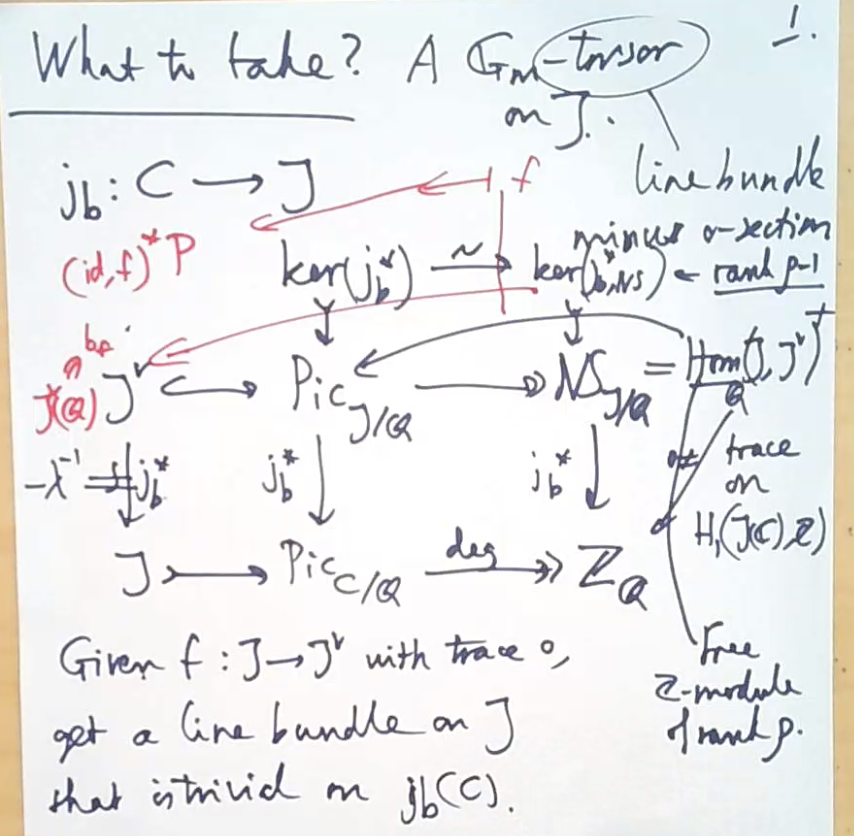
\includegraphics[width=0.5\textwidth]{../images/im5.png}
	\end{figure}


% Poincare Bundle
\subsection{Poincar\'e Bundle}

For all abelian varieties $A$, we can view $A^\vee$ as $\ext^1(A,\G_m)$, where
	\[
	\G_m \ma{} E \ma{\G_m \text{ torsor}} A
	\]
The maps $\G_m \to E$ are rigid: they have no non-trivial automorphisms that induce $\id_A$ and $\id_{\G_m}$. So over $A^\vee$, we have a universal extension 
	\[
	\begin{tikzcd}
	\G_{m,A} \arrow[hook]{r} \arrow{dr} & P^\times \arrow{d} \arrow[two heads]{r} &  A \times A^\vee \arrow{dl} \\
	& A^\vee & 
	\end{tikzcd}
	\]
$P^\times$ is also the universal extension of $A^\vee$ by $\G_m$ over $A$. So we have
	\[
	\begin{tikzcd}
	j_b^* T_{f} \arrow{r} \arrow{d} & T_{f \; r} \arrow{r} & P^\times \arrow{d} \\
	C \arrow{r}{j_b} \arrow{u} \arrow{ur}{j_b} & J \arrow{r}{(\id, \text{tr}_{b_f} \circ f)} & J \times J^\vee
	\end{tikzcd}
	\]
We know $J$ has dimension $g$ and $T_{f r}$ has dimension $g+1$. Take a $\Z$-basis $f_1, \ldots, f_{j-1}$ of $\ker(j_{b??}^*)$, gives
	\[
	\begin{tikzcd}
	& T \arrow{r} \arrow{d} &  (P^\times)^{j-1} \arrow{d} \\
	C \arrow{r}{j_b} \arrow{ur}{\tilde{j}_b} & J \arrow{r}{(\id,\tr_{b_{f_1}} \circ f_1, \ldots, \tr_{b_{f_1}})} & J \times (J^\vee)^{p-1} 
	\end{tikzcd}
	\]
Now $(P^\times)^{j-1}$ is a $\G_m^{p-1}$ torsor and $T$ has dimension $g+p-1$. We play the Chabauty game in $T$. We hope that if it works that $r< g+p-1$. (most wanted example have $p= g$). Now $T(\Q)$ is a $\Q^{\times,p-1}$-torsor.
	\[
	\begin{tikzcd}
	T(\Q) \arrow{d} \\
	J(\Q)
	\end{tikzcd}
	\]
Now $\Q^\times= \{\pm 1\} \times \Z$ (set of primes). There is a big problem: there are too many $\Q$-points in $T$. As a solution, we extend the geometry over $\Z$, $\Z^\times= \{\pm1\}$. 


\begin{rem}
{\bfseries From now on, everything is over $\Z$}
\end{rem}


Let $C$ be a proper, regular model of $C_\Q$, and let $J$ be the N\'eron model of $J_\Q$. Let $J^\vee$ be the N\'eron model of $J_\Q^\vee, J^{\vee,0} \subset J^\vee$, is the fiberwise connected component of $\alpha$. Now $P^\times$ is the unique extension of $P^\times_\Q$ to $J \times J^{\vee,0}$ as a bi-extension.


Now $P^\times$ is a $\G_m$-biextension of $A \times A^\vee$. Then there are two partial group laws, given by what we have already seen. For example, one of them is: if $x_1,x_2 \in A$, and $y \in A^\times$, i.e. $(x_1,y),(x_2,y) \in A \times A^\vee$, $z_1 \in P^\times(x_1,y)$, $z_2 \in P^\times(x_2,y)$, then we obtain $z_1 +_1 z_2 \in P^\times(x_1+x_2,y)$. 


We use the biextension structure of $P^\times$ over $J \times J^{\vee,0}$ to parametrize 
	\[
	\begin{tikzcd}
	T(\Z) \arrow{d} \\
	J(\Z) \arrow[bend left=40, dotted]{u}
	\end{tikzcd}
	\]
noting that $T(\Z)$ is a $(\pm 1)^{p-1}$-torsor. 
	\[
	\begin{tikzcd}
	C(\Z) \arrow{dd} \arrow{r} & T(\Z) \arrow[draw=none]{d}[sloped,auto=false]{\subseteq} \\
	& \ov{T(\Z)} \arrow[draw=none]{d}[sloped,auto=false]{\subseteq} \\
	C(\Z_p) \arrow{r} & T(\Z_p) 
	\end{tikzcd}
	\]
Now $C(\Z_p)$ is 1-dimensional, $g+p-1$-dimensional, and $\ov{T(\Z)}$ is at most $r$-dimensional. 

















 
% !TEX root = ../../../main/aws_chabauty.tex
\newpage
\subsection{Lecture 2}

% Correction to previous lecture???

Excuse the laziness, typesetting will come later for this lecture\dots

	\begin{figure}[!ht]
	\centering
	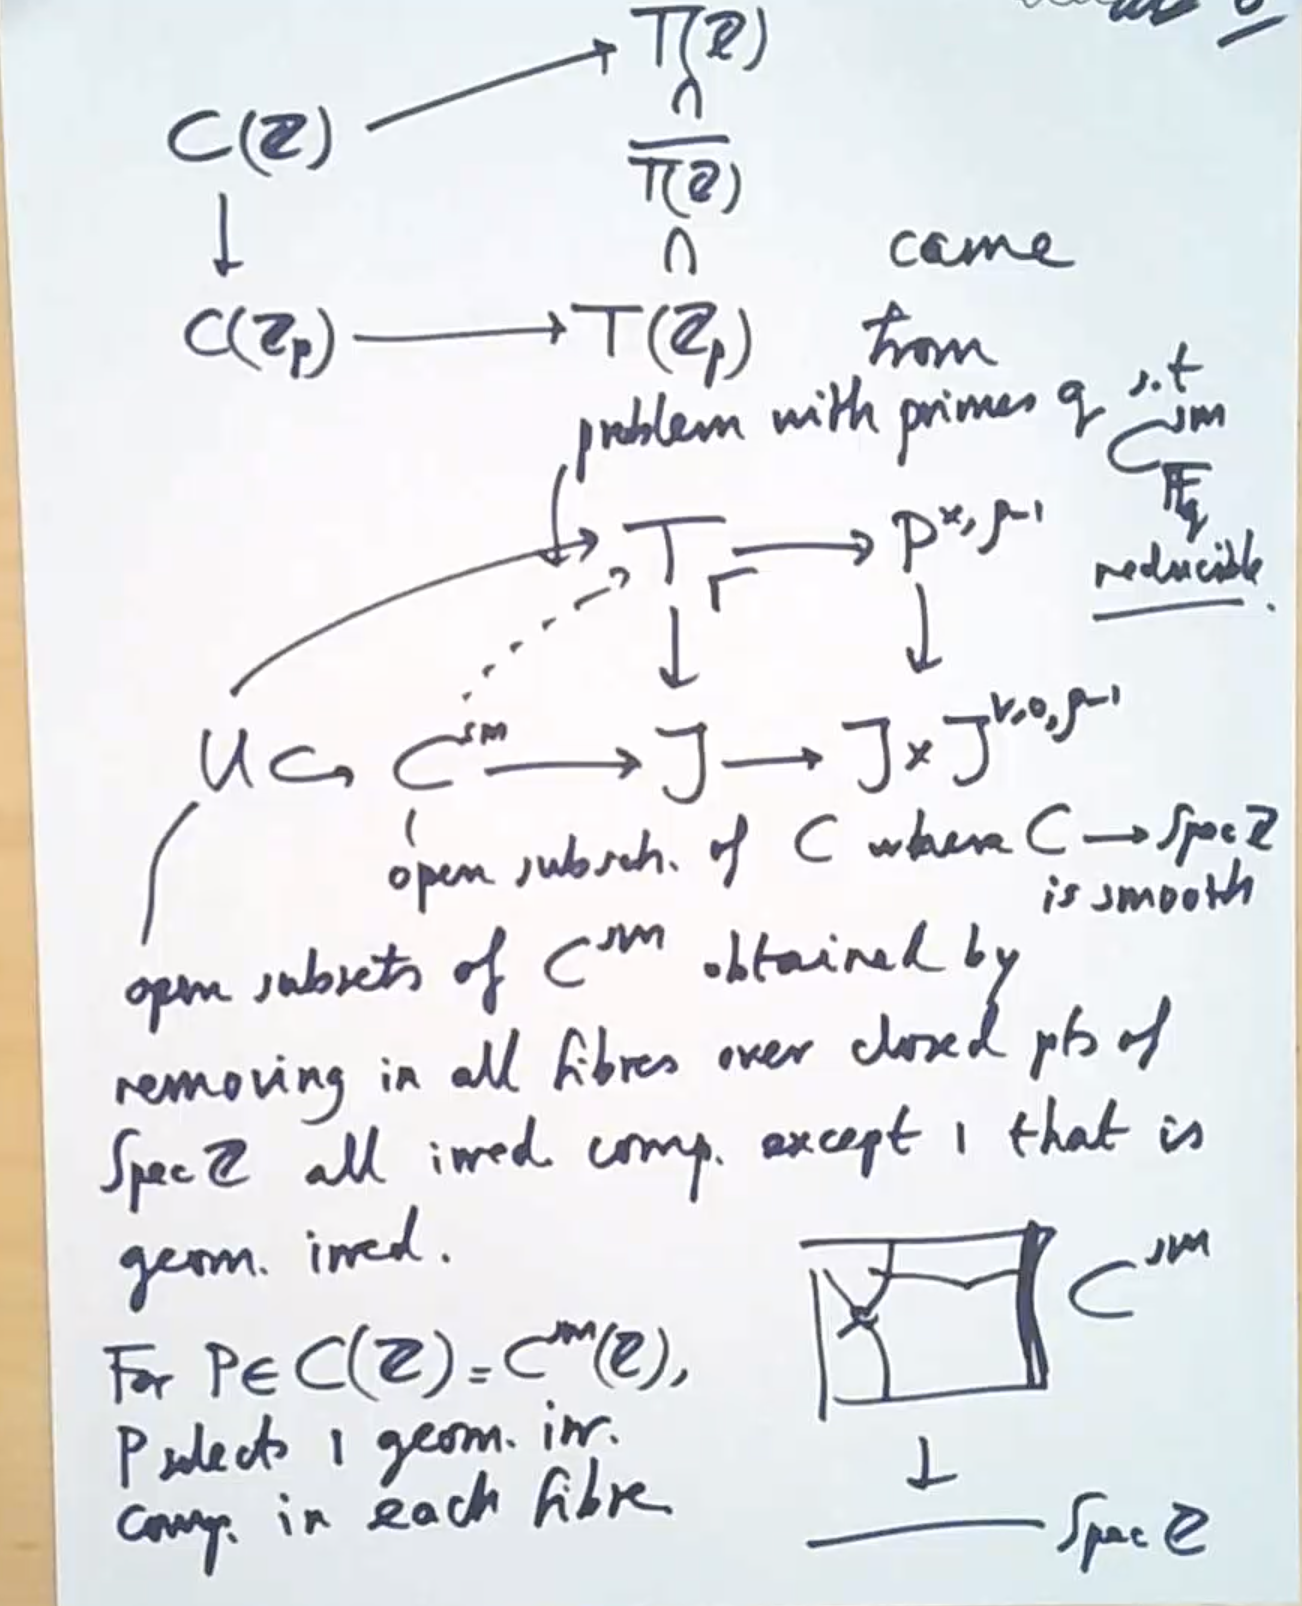
\includegraphics[width=0.5\textwidth]{../images/im12.png}
	\end{figure}


Say $n$ is the product of primes $q$ of bad reduction of $C/\Z$. Then $C \to \spec \Z$ is smooth over $\Z[1/n]$. These are finitely many of smooth $U$'s and $C_\Q= C^\text{sm}(\Z)= \sqcup_{\text{all }U\text{'s}} U(\Z)$.


\begin{ex}
$y^2+y= x^6 + \cdots$ (see section 8 of the notes). $n=3.43$, $C_{\F_{49}}^\text{sm}$ ind $C_{\F_j}^\text{sm}$. There are exactly 2 $U$'s.
	\begin{figure}[!ht]
	\centering
	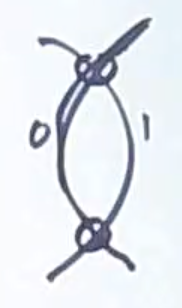
\includegraphics[width=0.1\textwidth]{../images/im13.png}
	\end{figure}
\end{ex}


	\begin{figure}[!ht]
	\centering
	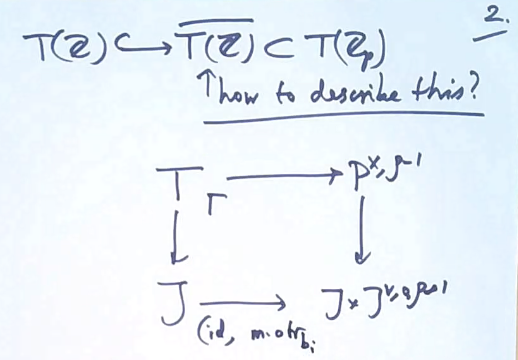
\includegraphics[width=0.5\textwidth]{../images/im14.png}
	\end{figure}


$J^{\vee,0} \hra J^\vee \twoheadrightarrow \Phi^\vee$, the group scheme of components of $J^\vee$. $\Phi^\vee$ trivial over $\Z[1/n]$. Finite \et fibers over $\Z/n\Z$. $m:=$ least common multiple of exponents of $\Phi^\vee(\tilde{\F}_q), q \mid n$. 


	\begin{figure}[!ht]
	\centering
	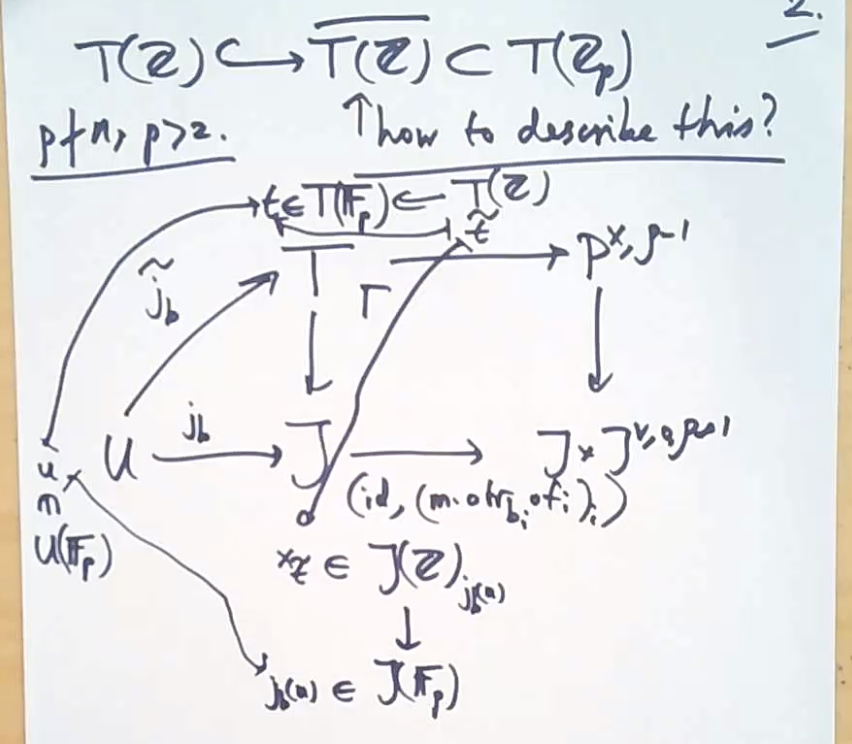
\includegraphics[width=0.5\textwidth]{../images/im15.png}
	\end{figure}


We want to create a map $J(\Z) \to T(\Z)$ but this is difficult because no such map comes from geometry. $J(\Z)_0 \cong \Z^r$, $x_1, \ldots, x_r$. We get a map $k_\Z: \Z^r \to T(\Z)_t$, not really surjective.


\begin{thm}[4.10]
	\[
	\Z^r \ma{k_\Z} T(\Z_p)_t \ma{\sim} \Z_p^{g+\rho-1}
	\]
where the bijection is given by evaluation at $1/p$ in the parametrization of $\O_{T,t}$. Note that $\Z^r \subset \Z_p^r$ is dense. There exists a unique $k=(k_1,\ldots,k_{g+\rho-1})$, $k_i \in \Z_p \langle z_1,\ldots,z_r \rangle= \Z_p[z_1,\ldots,z_r]^{\wedge p}$ and $\ov{T(\Z)}_t$ is the image of $k$. 
\end{thm}

\pf All of section 5, three and a half pages and lots of representations, $n \mapsto nP = \exp(n \log P)$. \qed \\


	\begin{figure}[!ht]
	\centering
	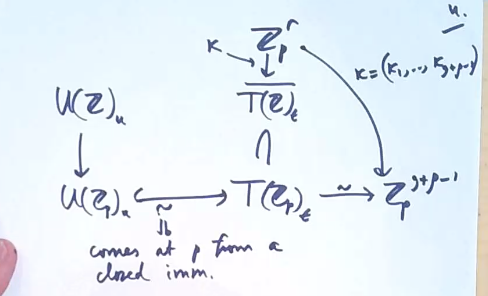
\includegraphics[width=0.5\textwidth]{../images/im16.png}
	\end{figure}


\begin{enumerate}[1.]
\item We want to pull back expressions fro the complete intersection $U \hra T$ and at $u$ get $g+\rho-2$ equations to $\Z_p^r$. 
\item We want to do this in terms of formal geometry, e.g. rings like $\Z_p \langle z_1,\ldots,z_r \rangle$, and then reduce $\mod p$, so we get polynomials in $\F_p[z_1,\ldots,z_r]$.
\end{enumerate}























% !TEX root = ../../../main/aws_chabauty.tex
\newpage
\subsection{Lecture 3}




































% !TEX root = ../../../main/aws_chabauty.tex
\newpage
\subsection{Lecture 4}





































% Kim
% !TEX root = ../../../main/aws_chabauty.tex
\newpage
\section{Minhyong Kim: Foundations of nonabelian Chabauty}
\subsection{Lectures 1--4}

Minhyong Kim's lectures were from his lecture note slides, please see those sections in Part~II. 

% Zureick-Brown
% !TEX root = ../../../main/aws_chabauty.tex
\newpage
\section{David Zureick-Brown: Effective Chabauty}
\subsection{Lecture 1}

\noindent Lorenzini-Tucker \par
\noindent McCollem-Poonen \par
\noindent Stoll \par
\noindent Katz-ZB \par\vspace{2\baselineskip}


\begin{thm}[K-ZB]
Let $X/\Q$ be a `nice' curve with $r= \rank J(\Q)$, and $p>2r+2$ a prime. Let $\fX$ be a regular proper minimal model of $X$. Let $r<g$, then 
	\[
	\#(X(\Q)) \leq \# \fX_{\F_p}^?(\F_p) + 2r
	\]
\end{thm}


\begin{thm}[Coleman, ``rank favorable bound'']
In the situation above, 
	\[
	\#(X(\Q)) \leq \# \fX_{\F_p}^?(\F_p) + (2g-2)
	\]
\end{thm}


A question of Mazur is can we bound $\#X(K)$ using the rank of $J(K)$ and $g$?


\begin{conj}[Uniformity Conjecture]
There exists $B(K,g)$ such that for all nice $X/K$ of genus $g$ with
	\[
	\#X(K) \leq B(K,g)
	\]
\end{conj}


Work of Poonen et al gives heuristics that, in the case of $X$ an elliptic curve, imply $r$ is bounded. 


The Weak Lang Conjecture states that if $X/K$ is a variety of general type, then there is $Z \subseteq X$ closed such that $Z(K) \subseteq X(K)$. 


\begin{thm}[Caparso,Harris,Mazur]
The Weak Lang Conjecture implies the Uniformity Conjecture
\end{thm}


\begin{ex}[Gordon-Grant, '93]
Let $X: y^2= x(x-1)(x-2)(x-5)(x-6)$. This is a hyperelliptic curve with $g= 2$ and rank 1. But $r=1 < 2$ so Coleman applies. Then $\#X(\Q)= 10$ GWP, 3 IG and IQ $\pm 120$. But mod 7, we have $\#X(\F_7)= 8$ gWP, $(3, \pm 6)$. 
	\[
	10 \leq \#X(\Q) \leq \#X(\F_7) + 2 = 8+2= 10
	\]
\end{ex}


\begin{thm}[Stoll]
Suppose that $X$ is hyperelliptic, and suppose that $r \leq g-3$. Then $\#X(\Q) \leq 3(r+4)(g-1) + \max\{1,4r\} \cdot g$.
\end{thm}


\begin{thm}[Katz-Rabinoff-ZB]
Suppose $r \leq g-3$. Then $\#X(\Q) \leq 84 g^2 - 98g + 28$. 
\end{thm}



% Effective Manin-Mumford
\subsubsection{Effective Manin-Mumford}

Let $X$ be a curve and $X \stackrel{i}{\hra} J$. Then $\#i(X) \cap J_\tor < \infty$, proven by Raynaud, Buildum, Coleman.

	\[
	X \hra J \ma{\log} \lie J
	\]
Then the integrals vanish on $X \cap J_\tors$. The nice thing here is that there is no necessary rank condition. 


\begin{thm}[KRZB]
\begin{itemize}
\item $(X \cap J_\tors)(\Q) \leq (?)$
\item $I$ and $X$ is very degenerate, e.g. totally degenerate
\end{itemize}
then we can bound $\# \cap J_\tors \leq ---$
\end{thm}


	\begin{figure}[!ht]
	\centering
	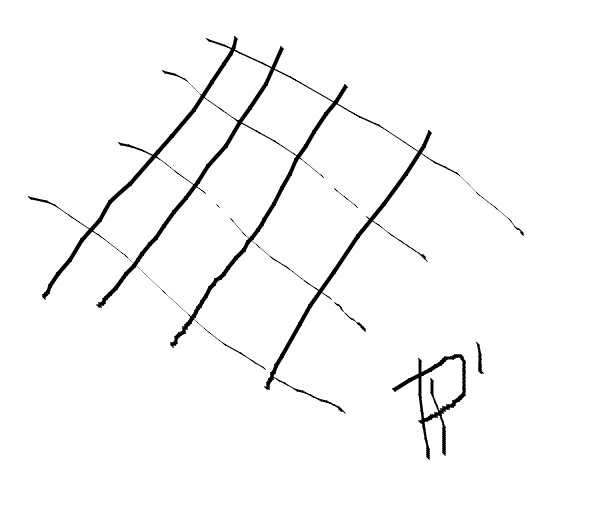
\includegraphics[width=0.3\textwidth]{../images/im2.png}
	\end{figure}
	
%	\begin{figure}[!ht]
%	\centering
%	\begin{tikzpicture}
%	\begin{axis}[
%	hide axis,
%	xmin=0, xmax=5,
%	ymin=0, ymax= 5
%	%rotate=45
%	]
%	\foreach \s in {-2,-1,0,1,2,3,4} {%
%		\addplot[domain=0:3,samples=50,black,thick] ({\x},{2-2*\x-\s}); 
%		\addplot[domain=0:3,samples=50,black,thick] ({\x},{2*\x+\s-4});
%	}
%	\end{axis}
%	\end{tikzpicture}
%	\end{figure}
	
	
	\[
	\begin{tikzcd}
	X(\Q) \arrow[hook]{r} & X(\Q_p) \arrow[hook]{d} \arrow{dr} \\
	J(\Q) \arrow[hook]{r} & J(\Q_p) \arrow{r}{\log} &  \lie J_{\Qp}
	\end{tikzcd}
	\]
where the log map is $D \mapsto (\omega \mapsto \int_Q^D \omega)$


`Black box Chabauty'.

\begin{itemize}
\item Setup
\item local analysis
\item global coordination 
\end{itemize}


Setup

Let $r<g$. There exists $V \subseteq H^0(X_{\Q_p}, \Omega^1)$ such that for all $P,Q \in X(\Q)$, $\int_P^Q \omega= 0$ for all $\omega \in V$ and $\dim V \geq g-r > 0$.


Local Analysis:

We can compute $\int_P^Q \omega$ locally and analyze with a Newton Polygon.

	\begin{figure}[!ht]
	\centering
	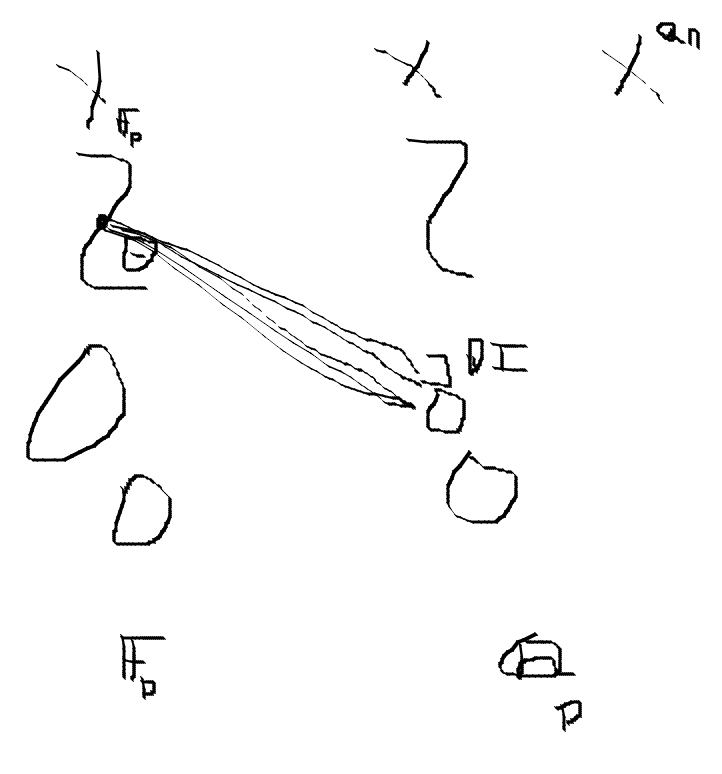
\includegraphics[width=0.3\textwidth]{../images/im3.png}
	\end{figure}

$[QI:= \{P \in X(\Q_p)$ such that $P \equiv Q \mod p \} \simeq p\Z_p$, the $p$-adic disc. Where the map is $p \mapsto u(P)$, where $u$ is a uniformizer at $\tilde{Q}$, a lift of $Q$.


\begin{ex}[HP survey]
$X: y^2= f(x)= x^6+8x^5+\cdots+1= xg(x)+1$.

$(0,1) \in X(\F_3)$.

$[(0,1)] \ma{\sim} p\Z_p$ with map $p \mapsto X(P)$ forward and $t \mapsto (t,\sqrt{tg(t)+1})$, which converges because $t$ is small, $\nu_p(t) > 0$. 
\end{ex}


To compute $\int_P^Q \omega$, only compute ``tiny'' integrals, i.e. $P=Q \mod p$. If $Q \in [P] \simeq p \Z_p \ni t$ with $\omega |_{[P]} = f(t) \;dt$ for some $f(t) \in \Z_p[1+1]$.
	\[
	\int_P^Q \omega= \int_Q^t f(t) \;dt = I(t)
	\]
integrating formally. 


























% !TEX root = ../../../main/aws_chabauty.tex
\newpage
\subsection{Lecture 2}

$\int$'s are locally analytic.

$P \in X(\F_p)$, $Q_1,Q_2 \in [P] \ma{\sim} P \hat{i} P$, given by $Q \mapsto t(Q)$, $t$ with respect to $P$.
	\[
	\int_{Q_1}^{Q_2} \omega= \int_{t_1}^{t_2} f(t) \;dt= \sum \dfrac{d_i t^{i+1}}{i+1} \bigg|_{t_1}^{t_2}= I_i(t)
	\]
by the Fundamental Theorem of Calculus.
	\[
	\omega \bigg|_{[P]}= f(t) \;dt= \sum a_i t^i, \quad a_i \in \Z_p
	\]


\begin{thm}[Coleman]
If $X/\Q$ is nice, $r<g$, and $p$ is a good prime with $p> 2g$, then $\#X(\Q) \leq \#X(\F_p) + 2g-2$.
\end{thm}


\pf Let $Q \in X(\F_p)$ and let $\omega \in V$ be a fixed annihilating differential. Let $n_\Q= \deg(\div \omega \cap [Q])$, then $\#\{z \in p \Z_p \colon I_i(z)=0 \} \leq 1+ n_\Q$. Then $\#X(\Q) \leq \#X(\Qp)_1$ (the $\Qp$ solutions to these integrals, i.e. the $\Qp$ points that vanish under the abelian integral). But this is at most $\sum_{Q \in X(\F_p)} (1+ n_\Q)$


	\begin{figure}[!ht]
	\centering
	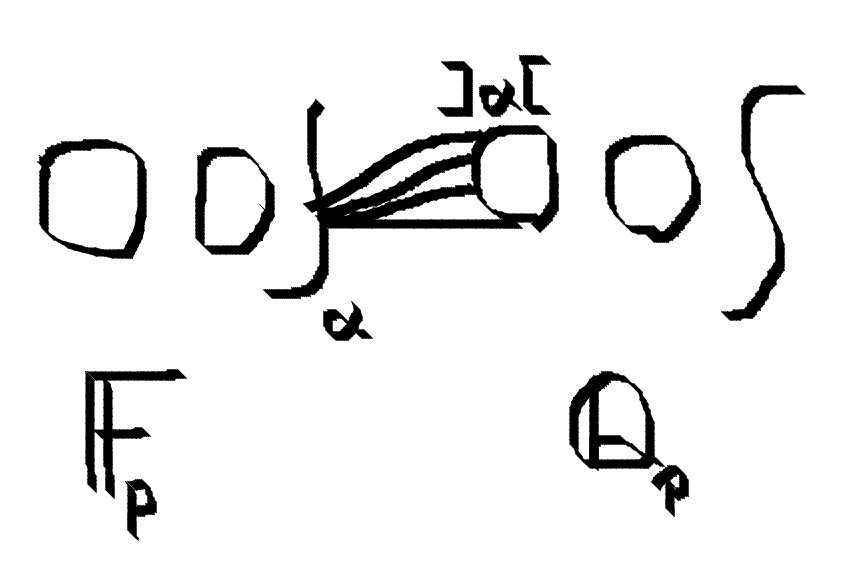
\includegraphics[width=0.4\textwidth]{../images/im6.png}
	\end{figure}


But then we have
	\[
	\begin{aligned}
	\#X(\Q) &\leq \#X(\Qp)_1 \\
	&\leq \sum_{Q \in X(\F_p)} (1+ n_\Q) \\
	&= \sum_{\alpha \in X(\F_p)} + \sum_{\alpha \in X(\F_p)} n_\Q \\
	&\leq \#X(\F_p) + \underbrace{2g-2}_{\deg \omega} 
	\end{aligned}
	\]
\qed \\


\begin{rem}
We did not really compute an upper bound on $\#X(\Q)$, but rather $\#X(\Qp)_1$, which is strictly larger. 
\end{rem}


\begin{lem}[Coleman]
Let $f(t)= \sum \dfrac{a_i}{i+1} \in \Qp[i+1]$ such that $f'(t)= \sum a_i t^i \in \Z_p[i+1]$. Let $m= \ord_{t=0} (f'(t) \mod p)$.\footnote{Note, $m=n_\Q$)} Suppose that $m < p-2$.\footnote{By the previous footnote, $p>m+2$ implies that $m \leq 2g-2$ by Riemann-Roch.} Then $f$ has at most $m+1$ zeros in $p \Z_p$. 
\end{lem}

\pf Newton polygons.

	\begin{figure}[!ht]
	\centering
	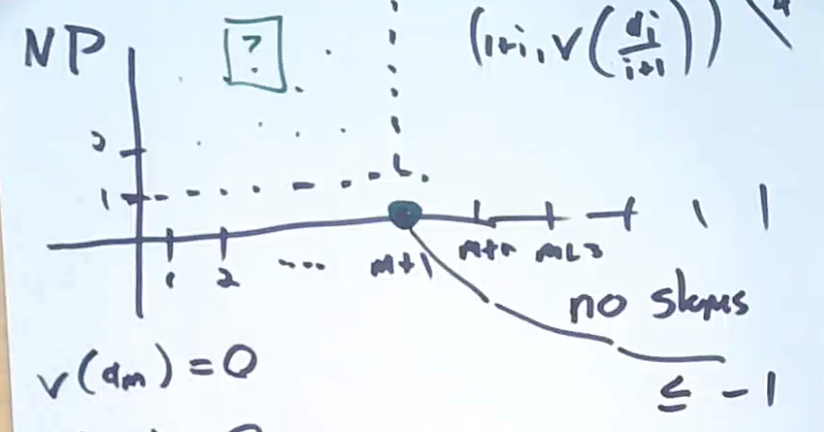
\includegraphics[width=0.5\textwidth]{../images/im7.png}
	\end{figure}
	

Note that $v(a_m)=0$. Because of the bound on $p$. Then $v(m+1)=0$. Then $v(a_i)>0$ for $i<m$ and $v(i+1)=0$ for $i<m$. But
	\[
	v\left( \dfrac{a_i}{i+1} \right) \geq v_p(i+1) > m+1 - (i+1)
	\]
Segments of slope $\alpha$ correspond to roots with valuation $-\alpha$. The length of the segment corresponds to the number of roots. \qed \\


If $X/\Qp$ is any variety, then $\trep X:= \ov{v(X(\ov{\Qp}))}$. 


\begin{ex}
$x+y= 1$, then
	
	\begin{figure}[!ht]
	\centering
	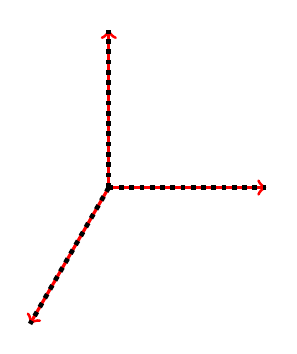
\begin{tikzpicture}
	
	\draw[line width=0.04cm,->,red] (0,0) -- (2,0);
	\draw[line width=0.04cm,->,red] (0,0) -- (0,2);
	\draw[line width=0.04cm,->,red] (0,0) -- (-1,-1.732);
	
	\draw[line width=0.06cm,dotted] (0,0) -- (2,0);
	\draw[line width=0.06cm,dotted] (0,0) -- (0,2);
	\draw[line width=0.06cm,dotted] (0,0) -- (-1,-1.732);
	
	\end{tikzpicture}
	\end{figure}
\end{ex}


\begin{ex}
$xyz= p(x^3+y^3+z^3)$
	\begin{figure}[!ht]
	\centering
	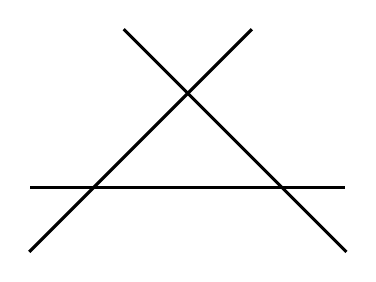
\begin{tikzpicture}[scale=2]
	\draw[line width=0.04cm] (-1,-0.3) -- (1,-0.3);
	\draw[line width=0.04cm] (-1.007,-0.707) -- (0.407,0.707);
	\draw[line width=0.04cm] (-0.407,0.707) -- (1.007,-0.707);
	\end{tikzpicture}
	\end{figure}

	\begin{figure}[!ht]
	\centering
	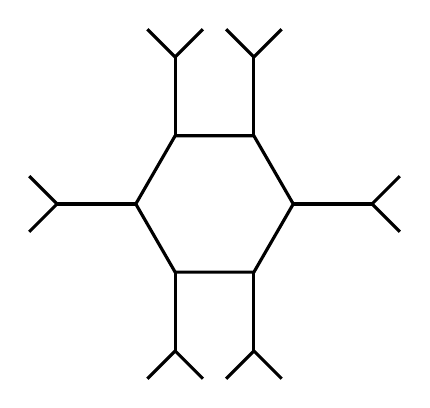
\begin{tikzpicture}[scale=1]
	\draw[line width=0.04cm] (1,0) -- (0.5,0.866) -- (-0.5,0.866) -- (-1,0) -- (-0.5,-0.866) -- (0.5,-0.866) -- (1,0);
	\draw[line width=0.04cm] (1,0) -- (2,0); 
		\draw[line width=0.04cm] (2,0) -- (2.353,0.353);
		\draw[line width=0.04cm] (2,0) -- (2.353,-0.353);
	\draw[line width=0.04cm] (0.5,0.866) -- (0.5,1.866);
		\draw[line width=0.04cm] (0.5,1.866) -- (0.853,2.219);
		\draw[line width=0.04cm] (0.5,1.866) -- (0.147,2.219);
	\draw[line width=0.04cm] (-0.5,0.866) -- (-0.5,1.866);
		\draw[line width=0.04cm] (-0.5,1.866) -- (-0.147,2.219);
		\draw[line width=0.04cm] (-0.5,1.866) -- (-0.853,2.219);
	\draw[line width=0.04cm] (-1,0) -- (-2,0);
		\draw[line width=0.04cm] (-2,0) -- (-2.353,0.353);
		\draw[line width=0.04cm] (-2,0) -- (-2.353,-0.353);
	\draw[line width=0.04cm] (-0.5,-0.866) -- (-0.5,-1.866);
	 	\draw[line width=0.04cm] (-0.5,-1.866) -- (-0.147,-2.219);
		\draw[line width=0.04cm] (-0.5,-1.866) -- (-0.853,-2.219);
	\draw[line width=0.04cm] (0.5,-0.866) -- (0.5,-1.866);
		\draw[line width=0.04cm] (0.5,-1.866) -- (0.853,-2.219);
		\draw[line width=0.04cm] (0.5,-1.866) -- (0.147,-2.219);
	\end{tikzpicture}
	\end{figure}
\end{ex}



% Stoll's Idea
\subsubsection{Stoll's Idea}

Choose the `best' $\omega$ for each $Q \in X(\F_p)$. Let $n_Q(\omega)= \deg(\div w(J \otimes L))$, $n_Q= \min_{W \in V} n_Q(\omega)$. 
	\[
	\#X(\Q) \leq \sum_{Q \in X(\F_p)} (1 + n_Q) \leq \#X(\F_p) + \sum_{Q \in X(\F_p)} n_Q
	\]
Now define $D:= \sum_{Q \in X(\F_p)} n_q[Q]$. We claim that $\deg D \leq 2r$. Now $\dim V \geq g-r$. Observe that $D$ is special. If $K_D$ is a canonical divisor, then $D$ is special if $\dim H^0(X,K \setminus D) \geq 1$. Then there exists same canonical divisor $K^1 \geq 0$ such that $D \leq K^1$. Now $\dim H^0(X,\Omega^1(-D)) >0$ containing $\omega$ if and only if $\div \omega \geq D$. 


\begin{thm}[Clifford]
If $D$ is special, then $\dim H^0(X,D) \leq \dfrac{\deg D}{\alpha} + 1$. 
\end{thm}


Context (Riemann-Roch). $h^0(D) - h^0(K-D)= \deg D+1-g$.

\pf $D= \sum n_q [Q]$.
	\[
	V \subseteq H^0(X_{\F_p}, \Omega^1(-D))
	\]
Then $g-r \leq \dim H^0(\Omega^1(-D)) \leq \frac{1}{2} (2g-2 - \deg D)+1$. But then $\deg D \leq 2r$. \qed \\


The notion of special is not good for singular curves. $H^0(D) \in P$. $K$ is not often special, there exist curves such that there does not exist an effective canonical divisor. 


	\begin{figure}[!ht]
	\centering
	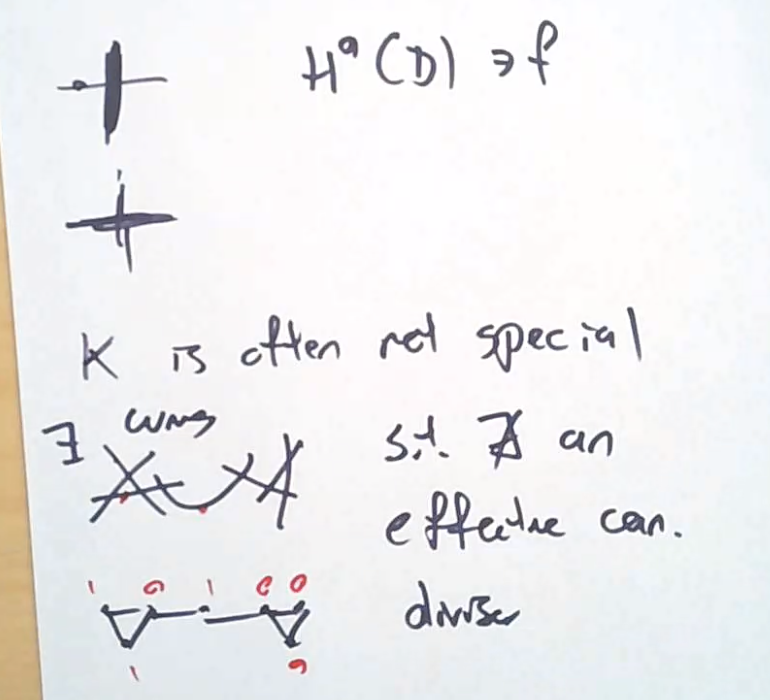
\includegraphics[width=0.5\textwidth]{../images/im11.png}
	\end{figure}




















% !TEX root = ../../../main/aws_chabauty.tex
\newpage
\subsection{Lecture 3}

	\begin{figure}[!ht]
	\centering
	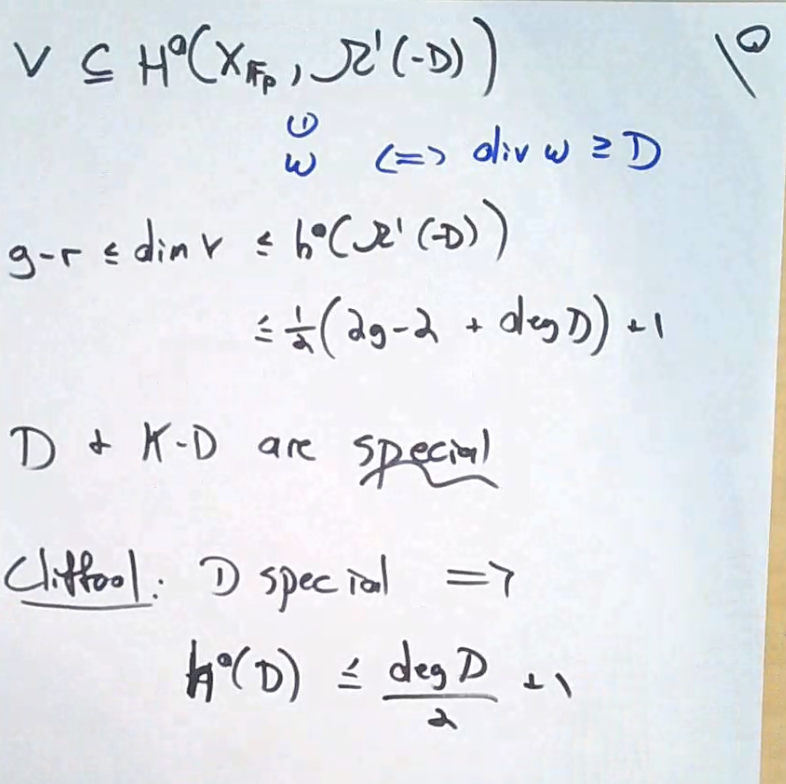
\includegraphics[width=0.5\textwidth]{../images/im17.png}
	\end{figure}
	
	\begin{figure}[!ht]
	\centering
	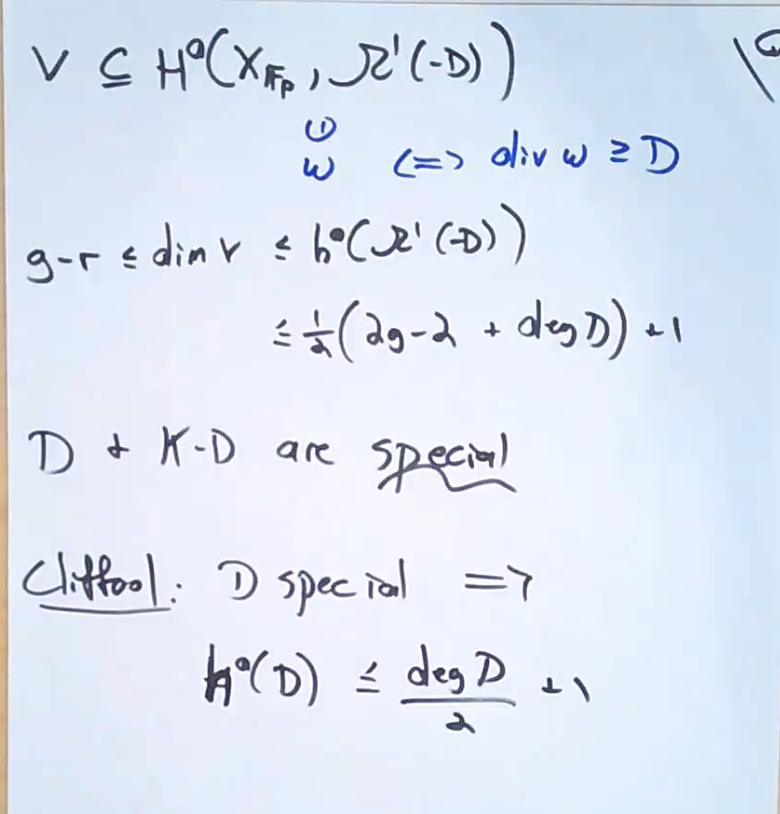
\includegraphics[width=0.5\textwidth]{../images/im18.png}
	\end{figure}
	
$|D|= \{ E \geq 0 \colon E \cap D \} \simeq \P^r$.

	\[
	\begin{aligned}
	r(D)&= -1 \quad \text{if } |D|= \emptyset \\
	r(D)&= 0 \quad \text{if } |D|\neq \emptyset \\
	r(D)&= 1 \quad \text{if } \forall P \in X, |D - P| \neq \emptyset \\
	r(D)&\geq i \quad \text{if } \forall E \geq 0 \text{ of deg }E \leq i, |D - E|\neq \emptyset 
	\end{aligned}
	\]
Then $X$ sm, then $r(D)= \dim H^0(X,D)-1$. If $X$ is singular, then $r(D) \neq \dim H^0(D)$


	\begin{figure}[!ht]
	\centering
	
\includegraphics[width=0.2\textwidth]{../images/im19.png}
	\end{figure}


The rank of $D$ is semicontinuous, i.e. if $\fX/E_P$, then $\fX_{\Qp} \to \fX_{\F_p}$ then $r(D) \geq r(D')$ [Hartshorne III.12]. 


	\begin{figure}[!ht]
	\centering
	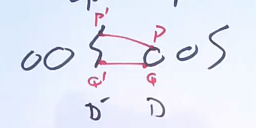
\includegraphics[width=0.4\textwidth]{../images/im20.png}
	\end{figure}


\begin{rem}
This inequality can be strict. If $P,Q \in X$ are not hyperelliptic, then reduces to $P',Q'= i(P)$, $h^0(P+Q)= 1$ and $h^0(P' + i(P))= 2$.
\end{rem}


\begin{dfn}[Regular]
Let $X$ be a scheme. We say that $X$ is regular if for all $P \in X$ corresponding to $\p$, we have $\dim_{k(\p)} \p/\p^2= \dim X$.
\end{dfn}


\begin{ex}
$y^2 - x^3- p/\Z_p$. 
	\[
	\begin{tikzcd}
	\fX \arrow{d}{\text{not sm}} \\
	\spec \Z_p
	\end{tikzcd}
	\]
$\fX$ is regular, $\fm= (x,y,p)$, $\fm/\fm^2= \langle x,y,p \rangle= \langle x,y \rangle$ PGM
\end{ex}


	\begin{figure}[!ht]
	\centering
	
\includegraphics[width=0.2\textwidth]{../images/im21.png}
	\end{figure}


If $\fX/\Z_p$ is a regular proper model of a sm curve
	\[
	\im( \fX(\Qp) \ma{\text{red}} \fX(\F_p) ) \subseteq \fX^{\text{sm}}(\F_p)
	\]


\begin{ex}
$y^2 - x^3 - p$, $[0,0]= \emptyset$, $y^2 - x^3 - p^2$, $[0,0]$ ? lop

Lorenzini-Tucker, Mc Poonen

regular, etc, $\fX$ r.p. model
	\[
	\#X(\Q) \leq \#\fX(\F_p) + 2g-2
	\]
The idea is the same proof:

	\begin{figure}[!ht]
	\centering
	
\includegraphics[width=0.5\textwidth]{../images/im22.png}
	\end{figure}
\end{ex}




\subsubsection{Matt Baker's Idea: Degenerate Even More}


	\begin{figure}[!ht]
	\centering
	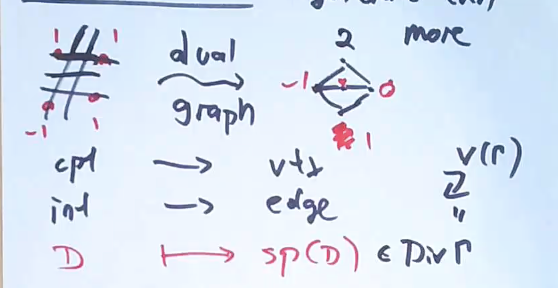
\includegraphics[width=0.5\textwidth]{../images/im23.png}
	\end{figure}



Baker, Baker-Norine

Notion of linear system, equivalence of divisors, and notion of rank, i.e. $|D|, r(D)$, $r(D) \leq r(\sp(D))$
	\[
	K_P= \sum (\deg v - 2)[v]
	\]
Notion of special RR and Clifford 


For Riemann-Roch, we have $r(D) - r(K_P - D)= \deg D + 1 - g$. Clifford gives if $D$ is special, then $r(D) \leq \frac{\deg D}{2}$. 


\begin{thm}[Katz,ZB]
Suppose $\fX$ is a regular proper model and $\fX_{\F_p}$ is totally degenerated. Then $\sp(D_{\text{ch}})$ is special
	\[
	D_{\text{ch}}= \sum n_\Q[\Q]
	\]
Actually, $r(K_P - D) \geq g - r - 1$.
\end{thm}

\pf (of rank favorability) $g - r - 1 \leq r(K_r - \sp(D)) \leq \frac{\deg(K_r - \deg D)}{2}= \frac{1}{2} (2g - 2 + \deg D)$. \qed \\



\subsubsection{Chip Firing}

Goal: Get (everybody) out of debt. 


	\begin{figure}[!ht]
	\centering
	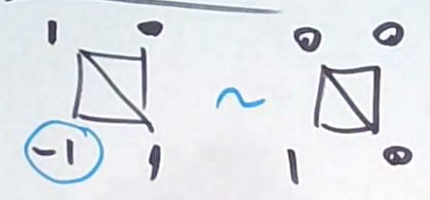
\includegraphics[width=0.5\textwidth]{../images/im24.png}
	\end{figure}
	
	\begin{figure}[!ht]
	\centering
	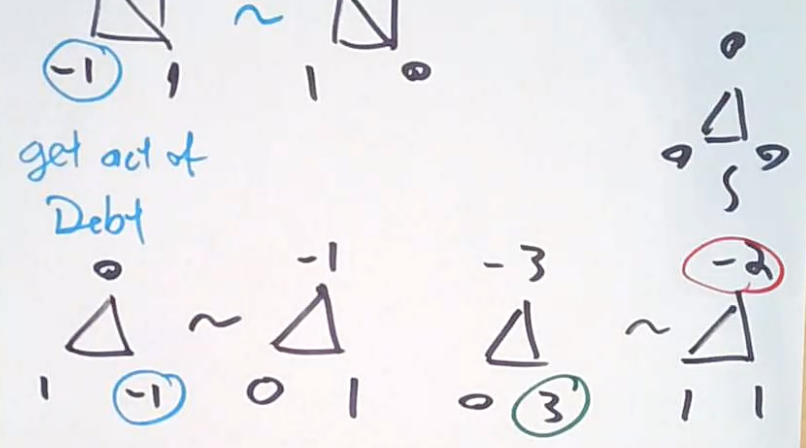
\includegraphics[width=0.5\textwidth]{../images/im25.png}
	\end{figure}


We say that $D \sim D^1$ if they differ by some sequence of loans and borrows. $\text{component group of special fiber of neron model } \simeq \pic^0 \Gamma \subseteq \pic \Gamma= \div \Gamma/\sim$.


$|D|= \{ D' \geq 0 \colon D' \sim D \}$. $r(D) \geq i$ if for all $E \geq 0$ with $\deg E \leq i$, $|D - E|\neq \emptyset$. 


	\begin{figure}[!ht]
	\centering
	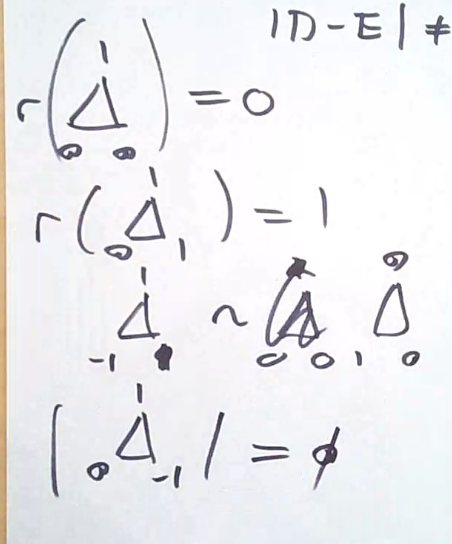
\includegraphics[width=0.5\textwidth]{../images/im26.png}
	\end{figure}


$\fX/\Z_p$, $\fX_{\F_p}= \cup C_i$, $\pic \fX \ma{\sp} \div \Gamma'$ given by $L \mapsto \sp(L):= \sum (\deg L \big|_{C_i})[v_i]$.

	\begin{figure}[!ht]
	\centering
	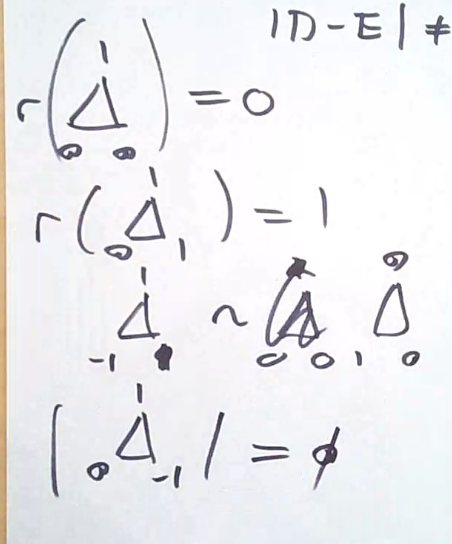
\includegraphics[width=0.5\textwidth]{../images/im26.png}
	\end{figure}


\begin{ex}
$L= \O(C_i)$
	\[
	\deg \O(C_i) \big|_{C_j}=
	\begin{cases}
	\# \text{ int points of } C_i \cap C_j \\
	\# \text{ self int of } C_i
	\end{cases}
	\]
$\fX_{\F_p}= (P)$ then $C_i \sim - \sum_{j \neq i} C_j$

$\sp(\O(C_i))$ if and only if firing at vertex $i$.
\end{ex}


\begin{ex}
$L= \omega_Z$.

Adjunction: $(\omega_\fX \otimes \O(C_i)) \big|_{C_i} \simeq \Omega^1_{C_i}$
	\[
	\begin{aligned}
	\deg \omega_\fX \big|_{C_i}&= \deg \Omega^1_{\P^1} - \deg \O(C_i) \big|_C \\
	&= -2 + \#\text{ int points of }C_i \text{ with rest }\fX \\
	&= K_p
	\end{aligned}
	\]

	\begin{figure}[!ht]
	\centering
	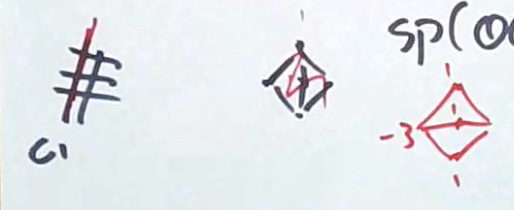
\includegraphics[width=0.5\textwidth]{../images/im28.png}
	\end{figure}
\end{ex}


As an upshot,

	\begin{figure}[!ht]
	\centering
	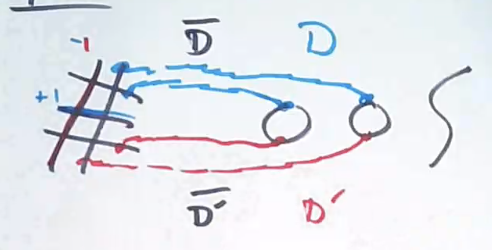
\includegraphics[width=0.5\textwidth]{../images/im29.png}
	\end{figure}

$D \sim D'$ on $\fX_{\sp}$, $\div f= D - D'$, $f: \fX_{\sp} \to \P^1$, extend $f$ to $\fX \leftrightarrow F$. Then $\div F= \ov{D} - \ov{D}' + \sum \alpha_i C_i$. The equivalence $\sp(\ov{D})$ with $\sp(\ov{D}')$ is witnessed by lending at $C_i(v_i)$ $\alpha_i$ many times. 


	\begin{figure}[!ht]
	\centering
	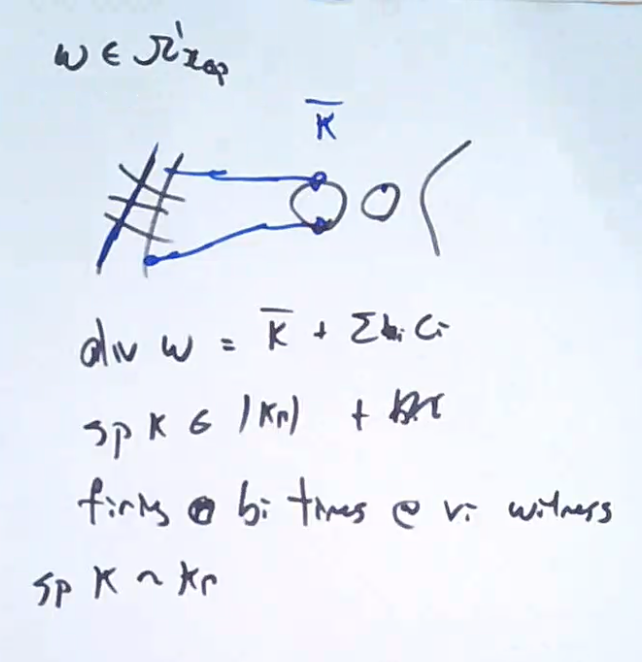
\includegraphics[width=0.5\textwidth]{../images/im30.png}
	\end{figure}





























% !TEX root = ../../../main/aws_chabauty.tex
\newpage
\subsection{Lecture 4}

	\begin{figure}[!ht]
	\centering
	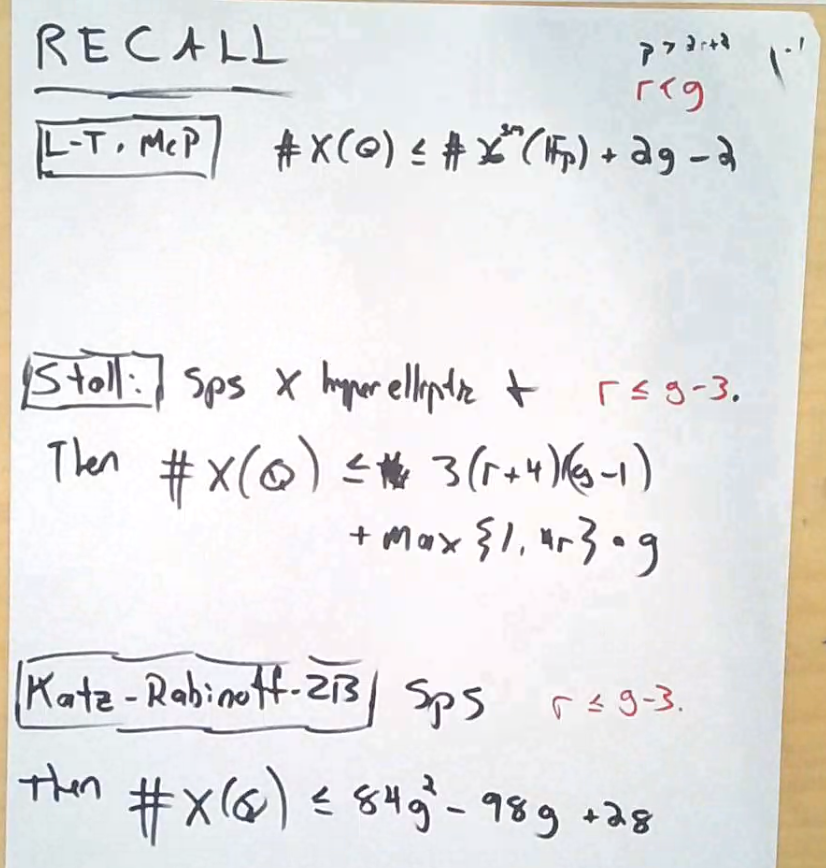
\includegraphics[width=0.5\textwidth]{../images/im34.png}
	\end{figure}

	\begin{figure}[!ht]
	\centering
	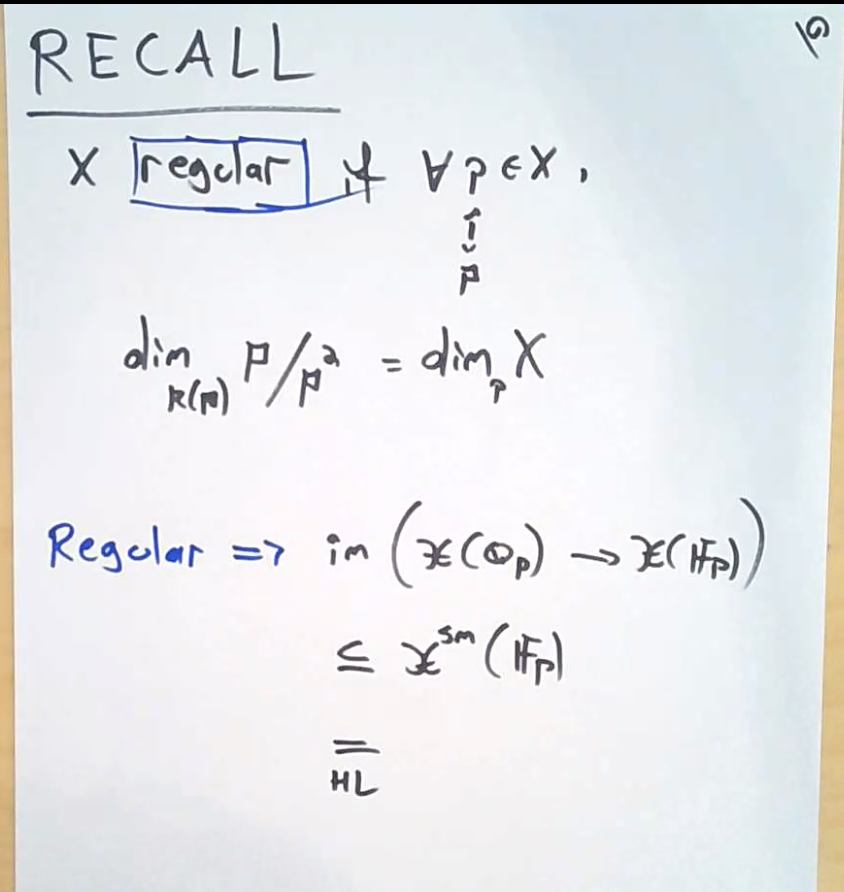
\includegraphics[width=0.5\textwidth]{../images/im35.png}
	\end{figure}

Problem: $\fX^{\text{sm}}(\F_p)$ is unbounded. $xyz= p(x^3+y^3+z^3)$. 

	\begin{figure}[!ht]
	\centering
	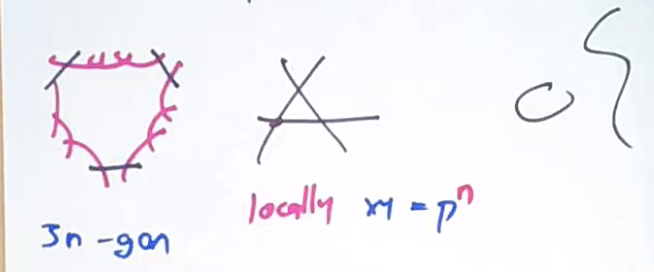
\includegraphics[width=0.5\textwidth]{../images/im36.png}
	\end{figure}

Stoll

\begin{itemize}
\item Work of non-regular model
\item cont. chains of $\P^1$'s
\item then $\fX(\F_p)$ is bounded via $p$ and $g$
\end{itemize}


Problem: Setup and local analysis is hard.


Main Tool: (KRZB)

Systematic use of Berkovich and tropical geometry

Setup, 2 types of $\int$'s
	\[
	\int_{\text{abelian}} + \int_{\text{Berk.-Coleman}}
	\]
The abelian integral comes from Lie $J$ and ????. The Berk.-Coleman integral is more computable and not equal to $\int_{\text{Ab}}$. The difference between the two is linear in $\omega$. The difference factors through Trop $T$, where $T$ is 
	\[
	\begin{tikzcd}
	& T \subseteq & \\
	A & \subseteq \tilde{J} \arrow[two heads]{d} \arrow{r} & J^? \\
	& A \text{ good red}
	\end{tikzcd}
	\]

Local Analysis:

Potential then on $X^\text{an}$.


``Global Step''

``Combinatorial optimization for sections of ``Tropical Canonical bundle''''

Tay version:

$|K \Gamma| \ni D$, bound for the min \# of things for which witness $D \sim K_P$.


Time travel to AWS 2007.

The Gelfand spectrum
$M(R)= \{ R \ma{|\cdot|} \R\}$ set of bounded multi. seminorms 

There is a map $M(R) \to \R$ given by $|\cdot| \mapsto |f|$. 

If $x \in M(R), f \in R$, write ``$f(x):= |f|$''. 


\begin{ex}
Let $\Q_p\{t\} = \sum_{i=0}^\infty a_i t^i$, where $a_i \in \Qp$ with $|a_i| \to 0$. Now$M(\Qp\{t\}) \supseteq \text{max spec } \Qp\{t\} \in x \in \ov{\Z}_p \subseteq \ov{\Q}_p$. 

	\begin{figure}[!ht]
	\centering
	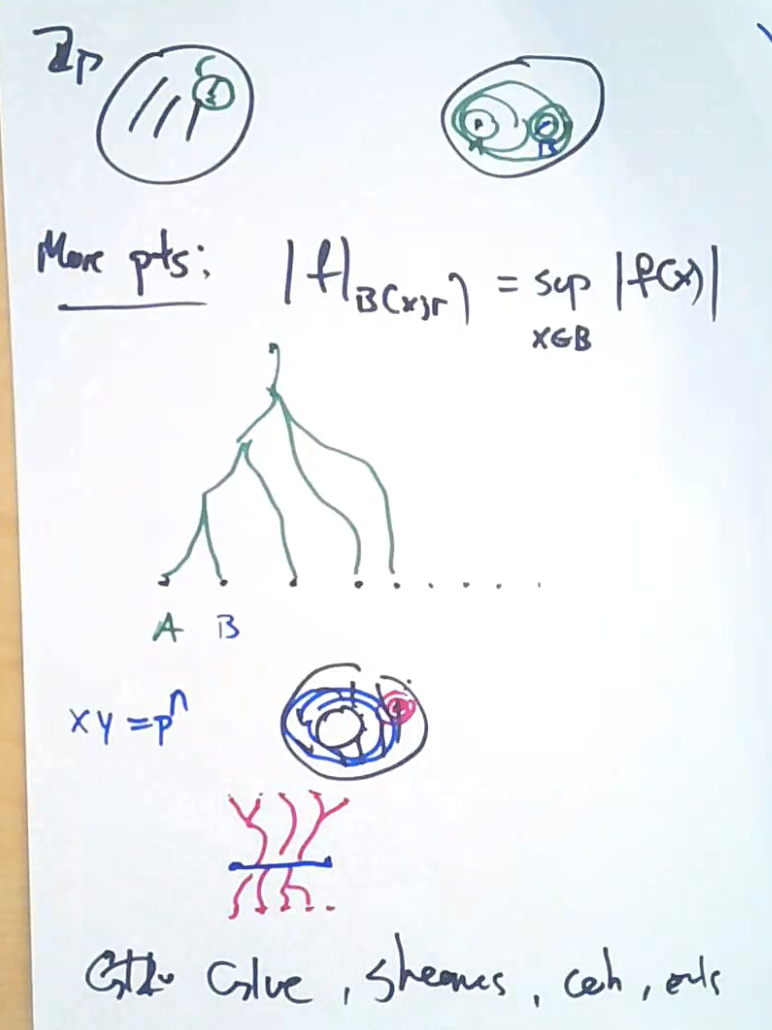
\includegraphics[width=0.5\textwidth]{../images/im37.png}
	\end{figure}

Max points: $|f|_{B(x|f)}= \sup_{x \in B} |f(x)|$
\end{ex}


Fundamental Theorem of Tropical Geometry:

Baker-Payne-Rabinoff
Berkovich, Thuiller

$\fX/\Z_p$ s.stable

$xyz= p(x^3+y^3+z^3)$.


	\begin{figure}[!ht]
	\centering
	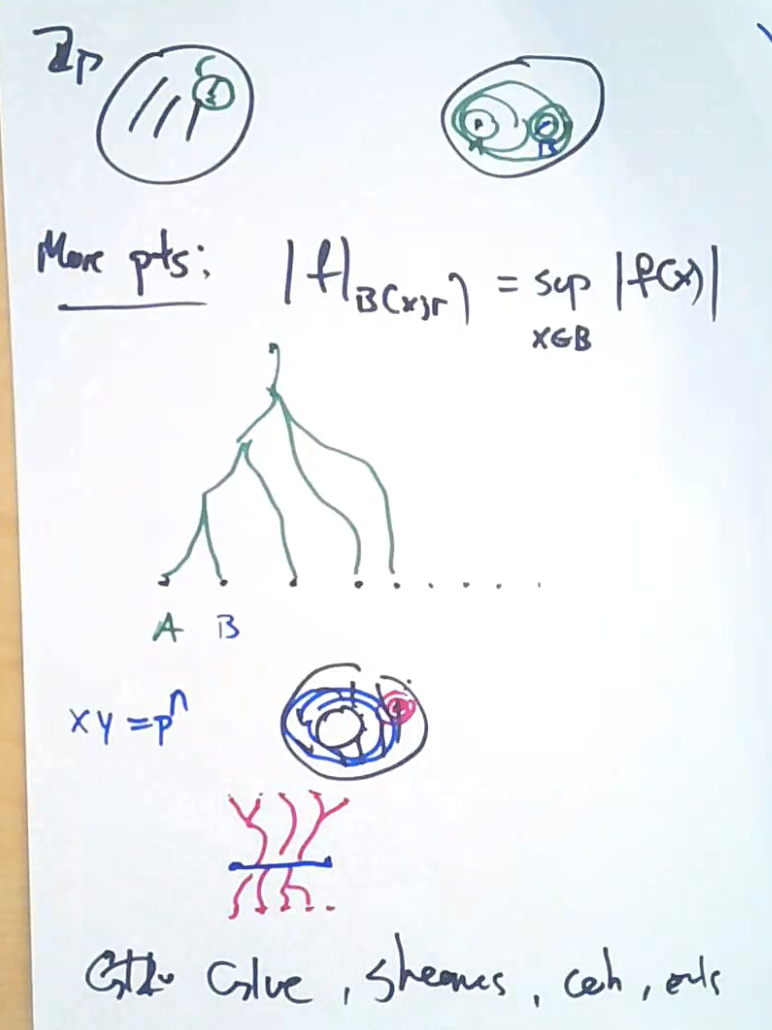
\includegraphics[width=0.5\textwidth]{../images/im37.png}
	\end{figure}

Potential Thm:

$\fX \ma{\text{an }f} \P^1$

$F(x)= - \log|f(x)|$, $F \big|_P$ is $P \big|_W$ linear


\begin{thm}
$\tau_* \div f= \div F:= \sum (\text{slope newton poly at }P) [P]$
\end{thm}


\begin{ex}
$f(x;y;z):= [x;z]$
$\div f= [0 \colon \xi_o \colon 1]= -([1 \colon \xi_0 \colon 0] + \cdots)$
$?????????$


% Rabinoff Utah survey paper photo

	\begin{figure}[!ht]
	\centering
	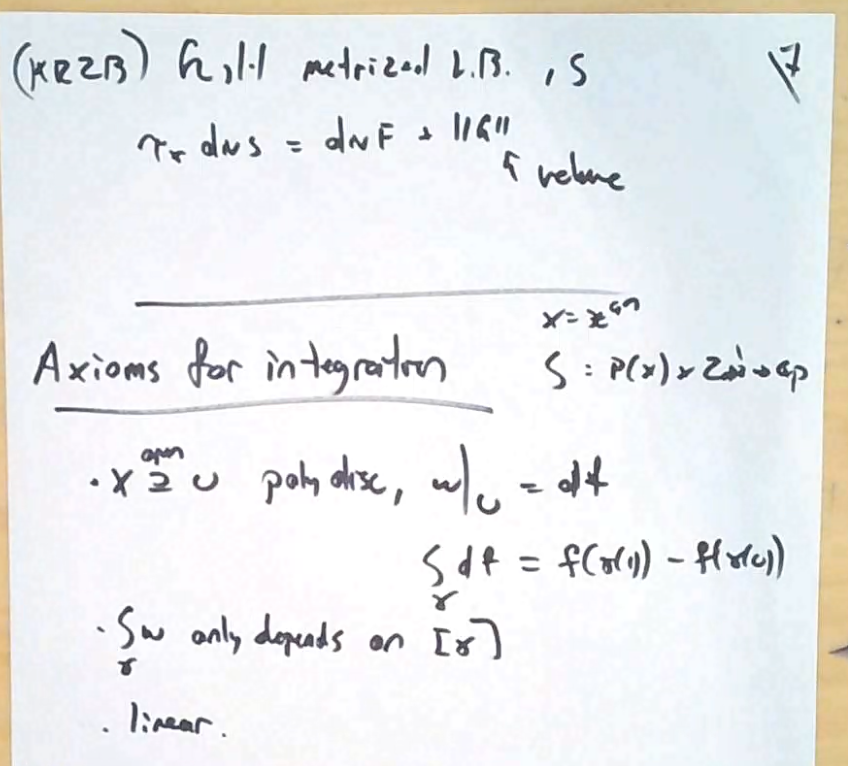
\includegraphics[width=0.5\textwidth]{../images/im40.png}
	\end{figure}
\end{ex}


	\begin{figure}[!ht]
	\centering
	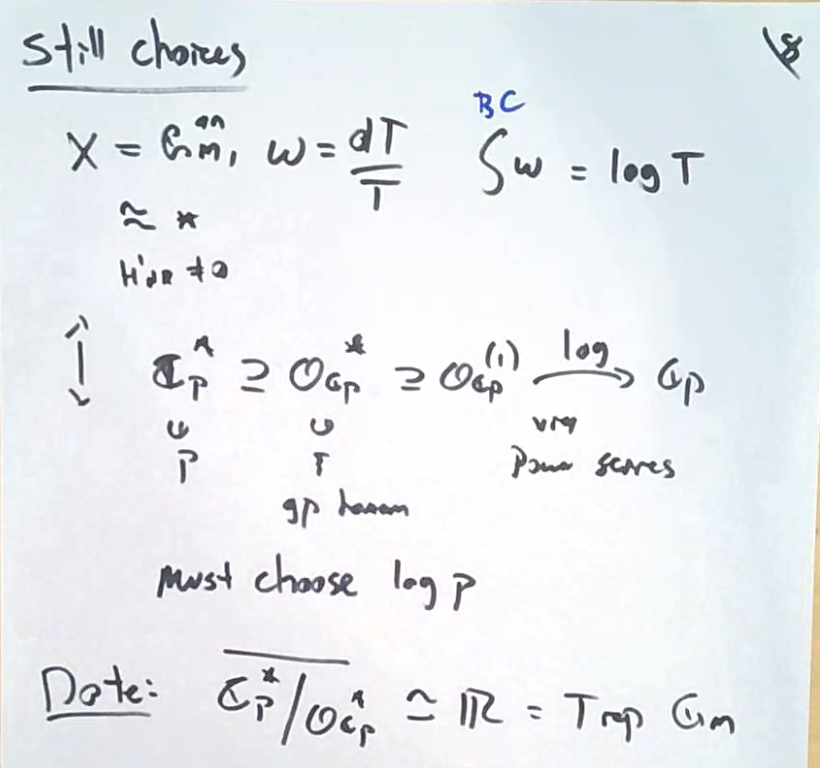
\includegraphics[width=0.5\textwidth]{../images/im41.png}
	\end{figure}

	\begin{figure}[!ht]
	\centering
	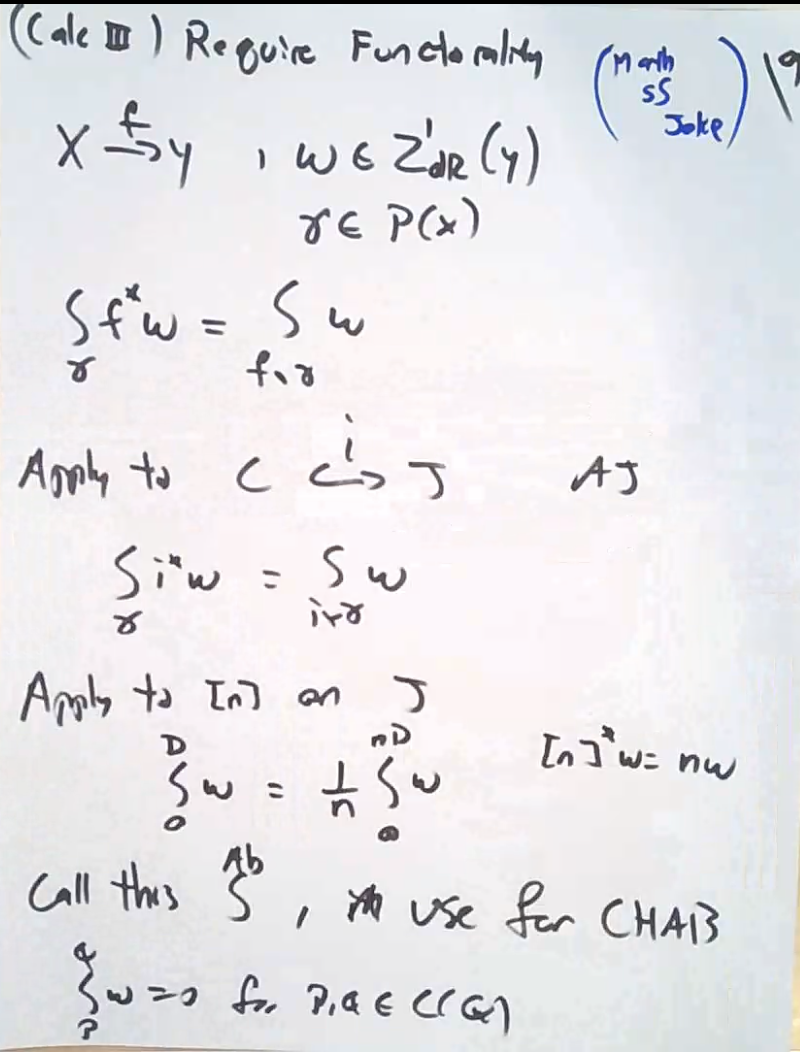
\includegraphics[width=0.5\textwidth]{../images/im42.png}
	\end{figure}

	\begin{figure}[!ht]
	\centering
	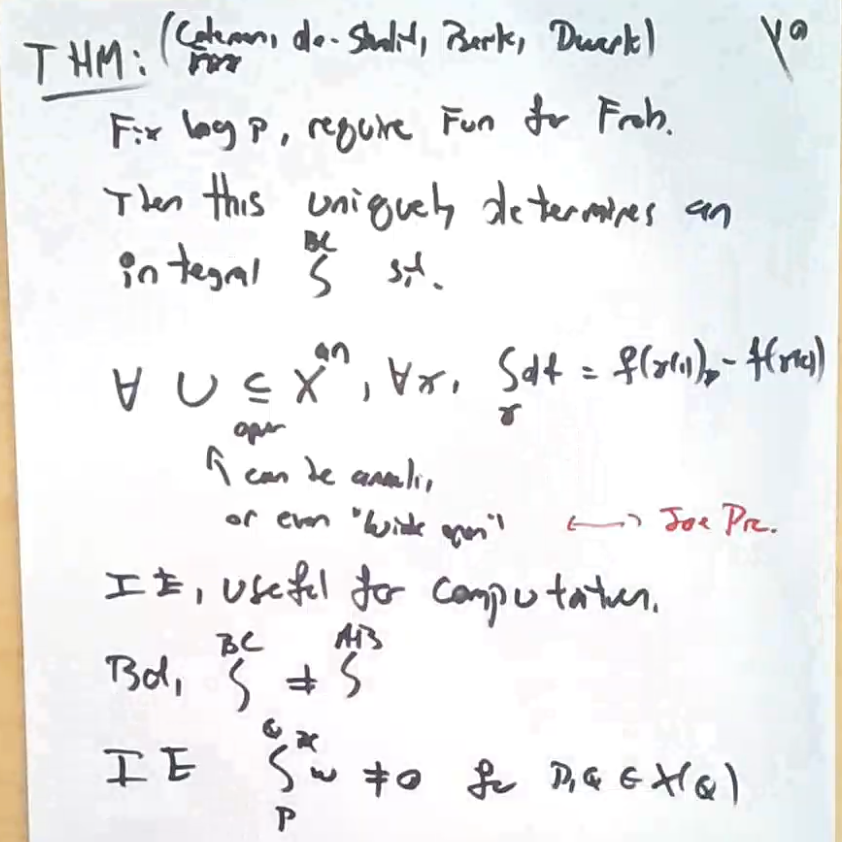
\includegraphics[width=0.5\textwidth]{../images/im43.png}
	\end{figure}


	\begin{figure}[!ht]
	\centering
	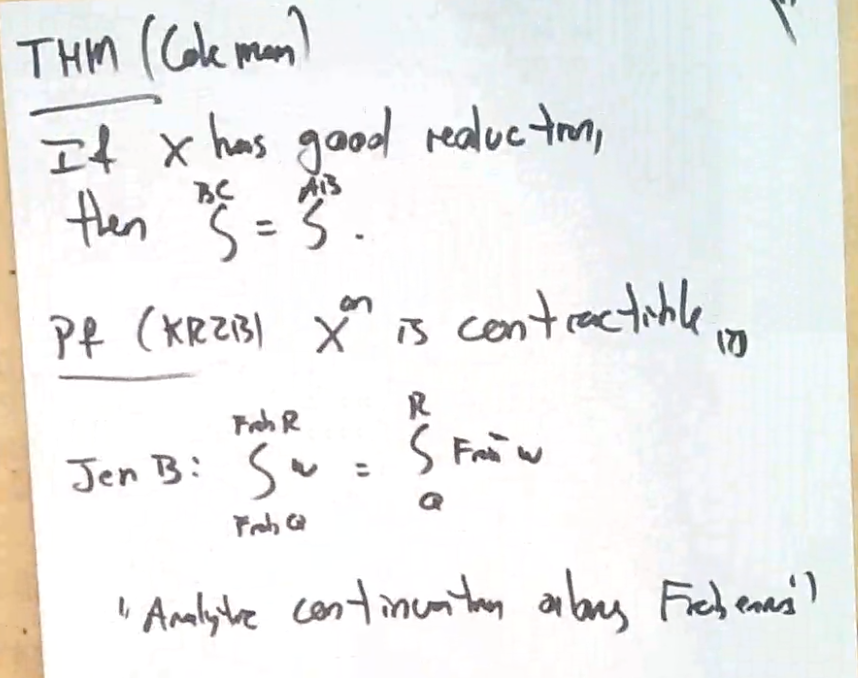
\includegraphics[width=0.5\textwidth]{../images/im44.png}
	\end{figure}

	\begin{figure}[!ht]
	\centering
	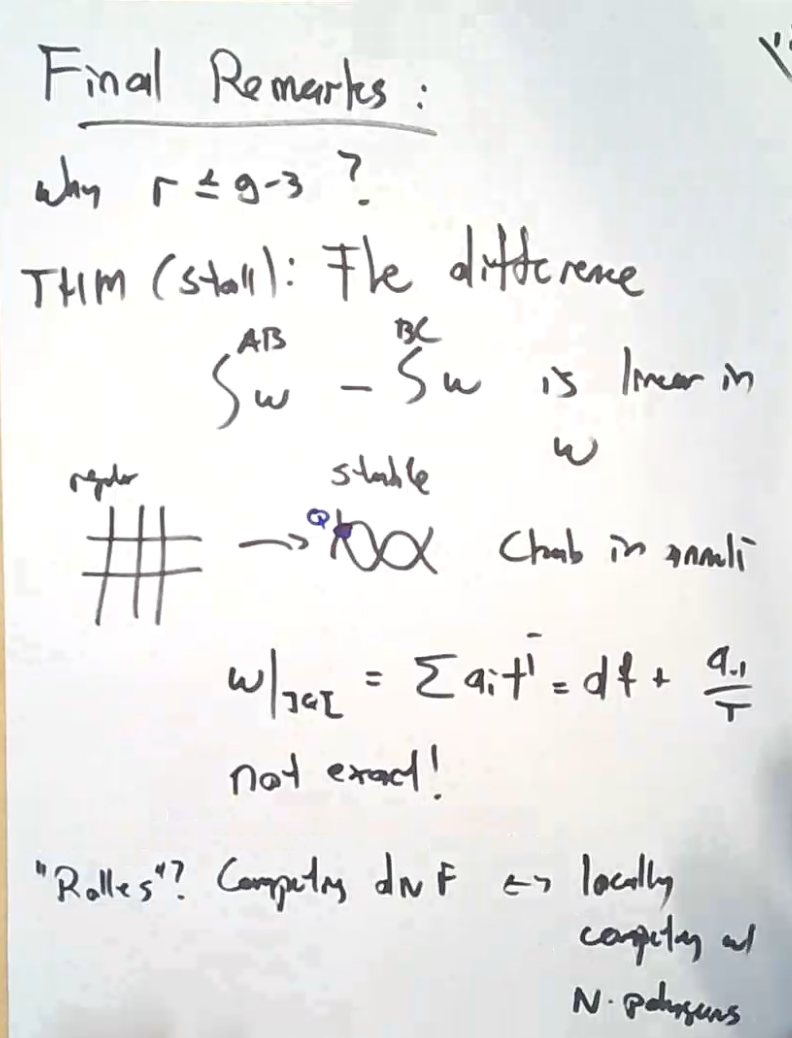
\includegraphics[width=0.5\textwidth]{../images/im45.png}
	\end{figure}





























% -------------------
% Course/Project Outlines
% -------------------
\ifbool{notesonly}{}{%
\newpage
\thispagestyle{empty}
\part{Course/Project Outlines \& Lecture Notes}
\newpage

%\setcounter{section}{1}

% Poonen
\phantomsection
\addtocounter{section}{1}
\addcontentsline{toc}{section}{\protect\numberline{\thesection} Bjorn Poonen}
\phantomsection
\setcounter{subsection}{1}
\addcontentsline{toc}{subsection}{\protect\numberline{\thesubsection} Lecture Notes}
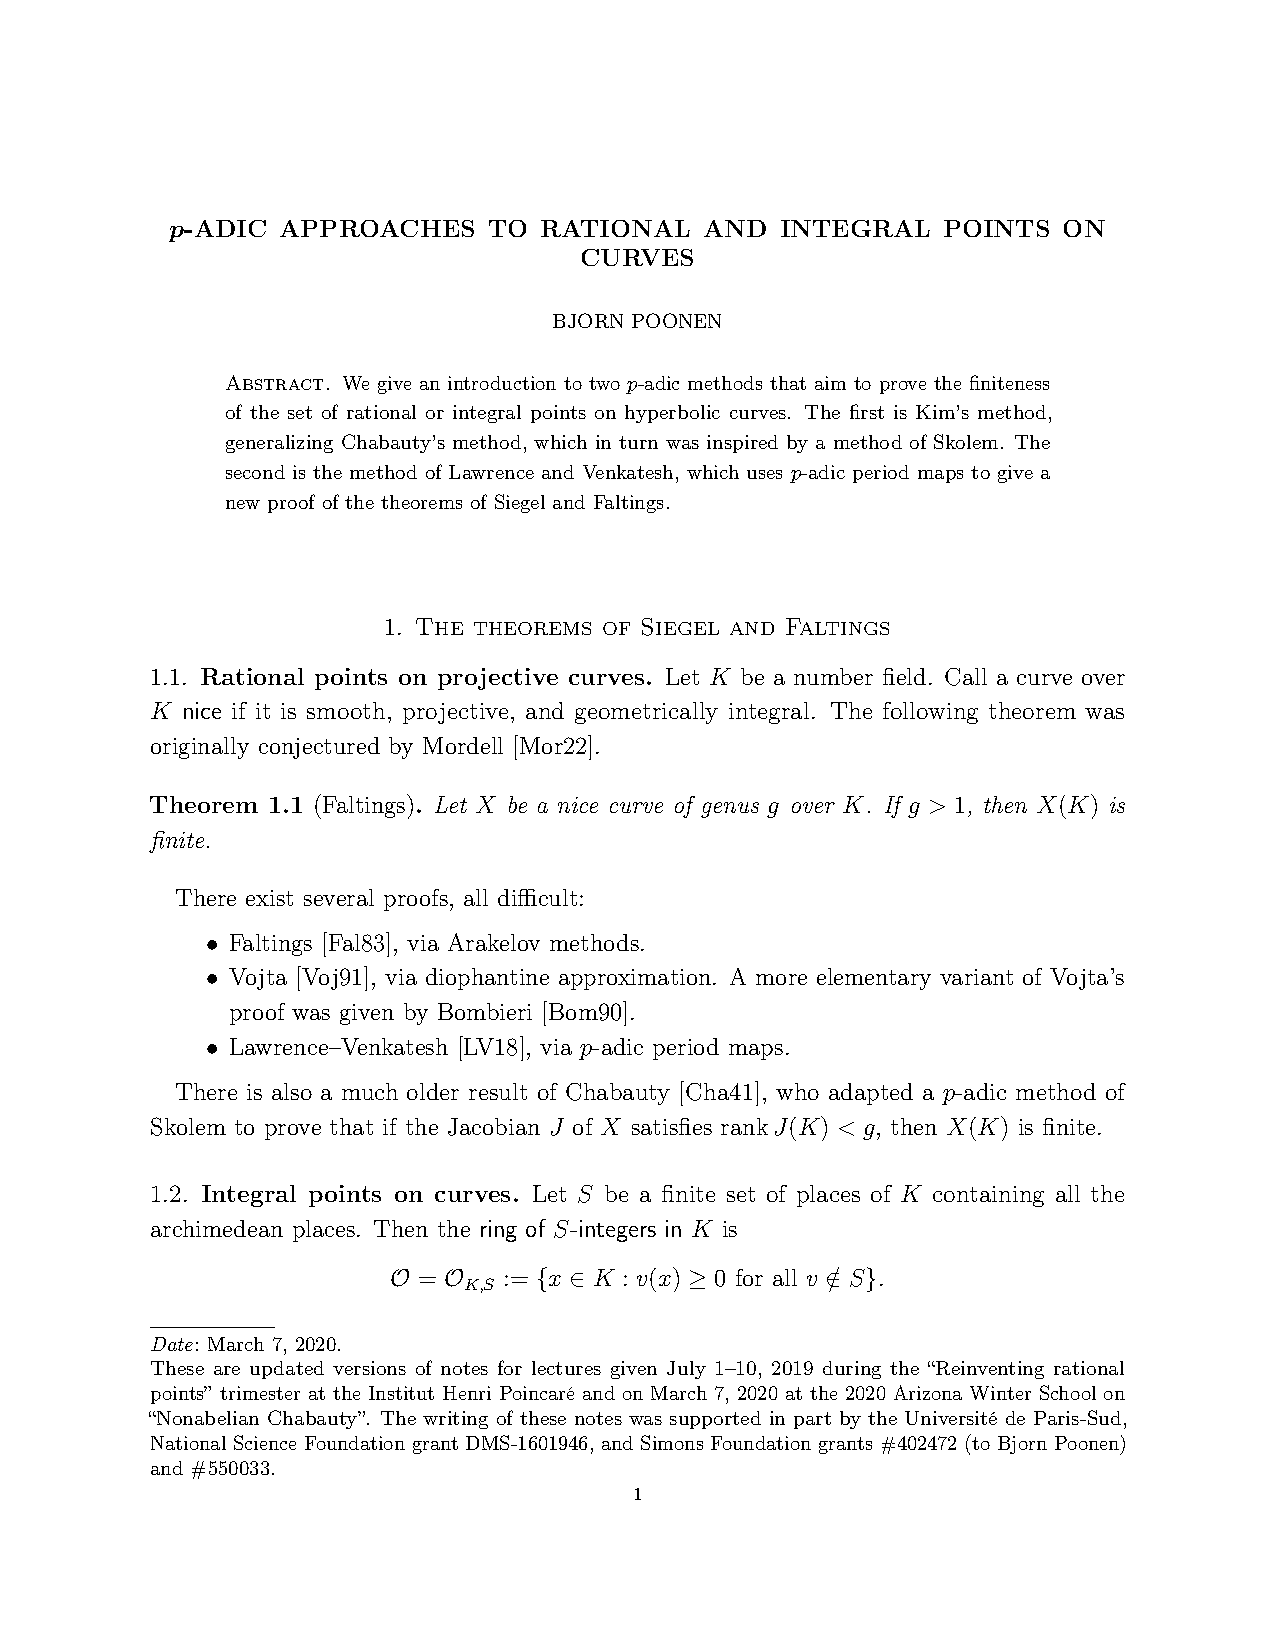
\includepdf[pages=-,scale=1,pagecommand={\thispagestyle{normal}}]{../notes/poonen/p-adic_approach.pdf}

% Balakrishnan
\phantomsection
\addtocounter{section}{1}
\addcontentsline{toc}{section}{\protect\numberline{\thesection} Jennifer Balakrishnan: Computational tools for quadratic Chabauty}
\phantomsection
\setcounter{subsection}{1}
\addcontentsline{toc}{subsection}{\protect\numberline{\thesubsection} Course \& Project Outline}
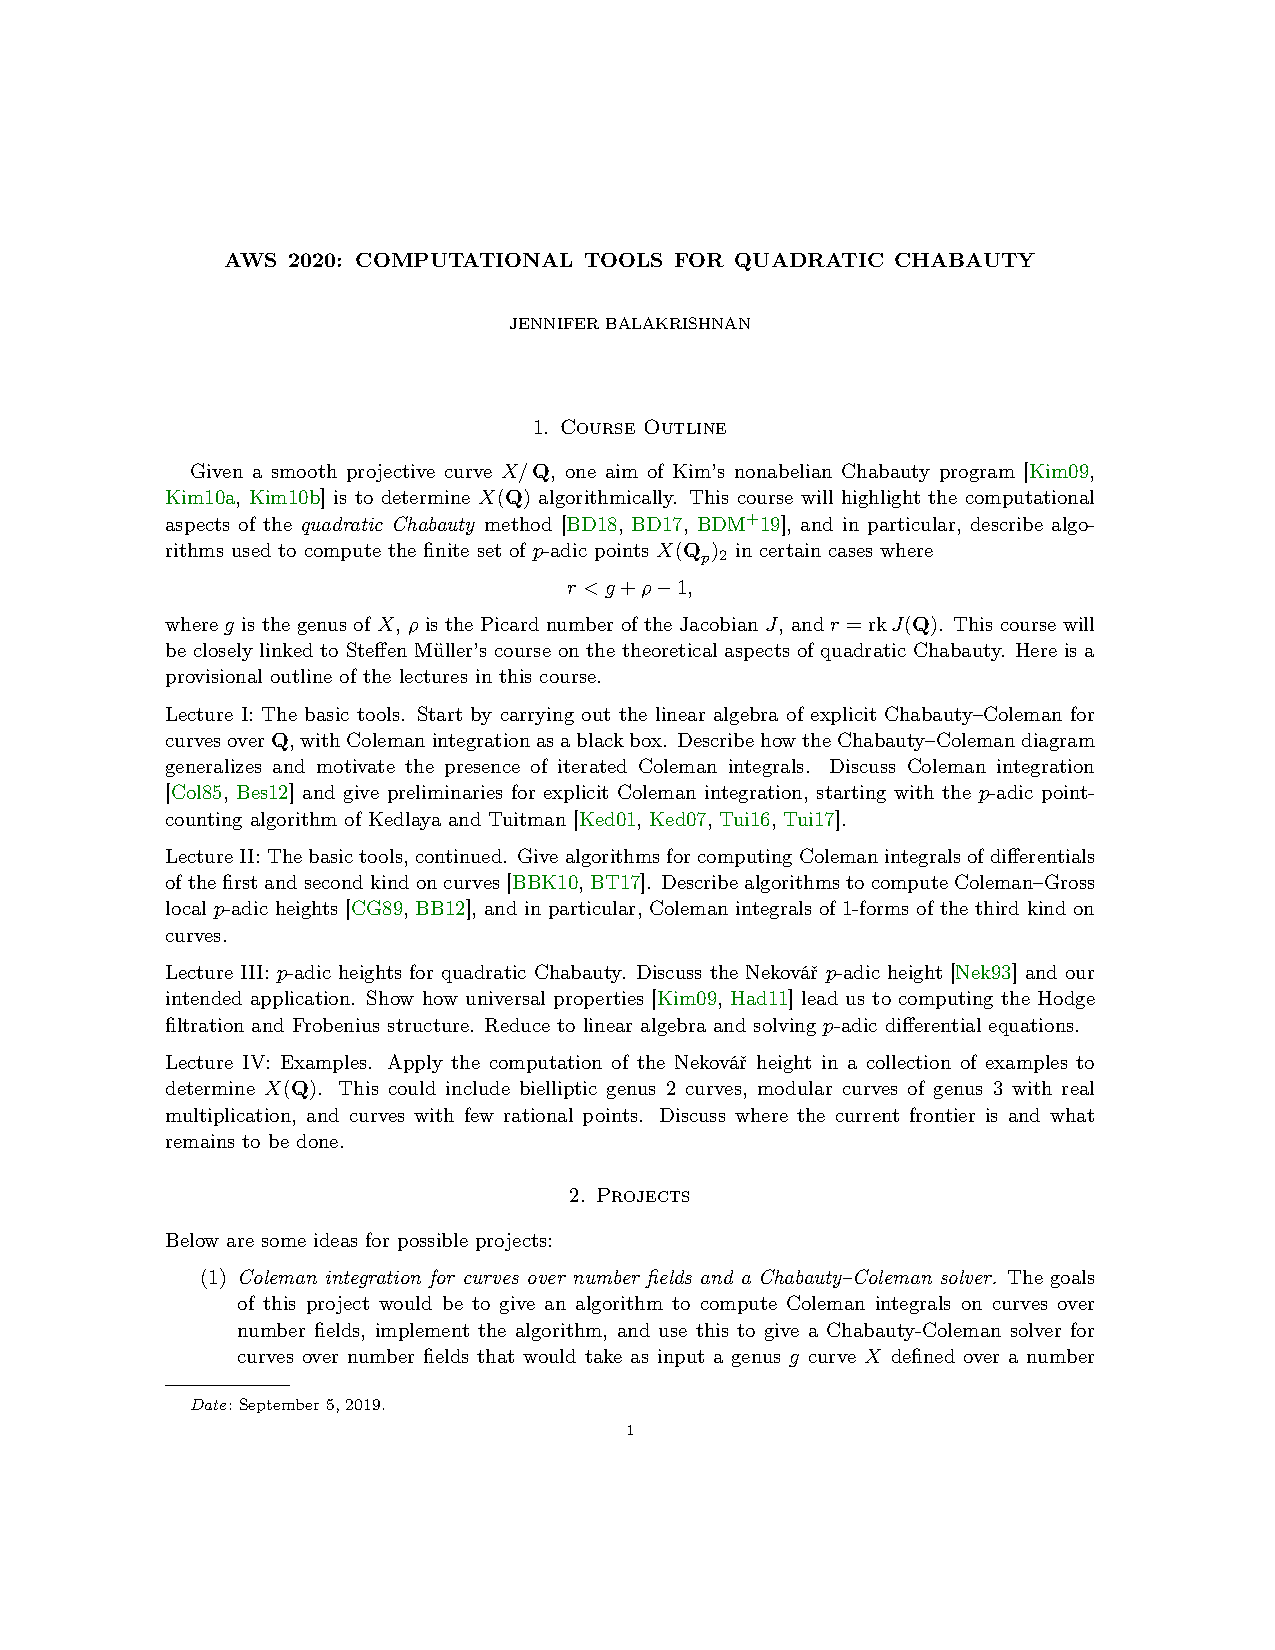
\includepdf[pages=-,scale=1,pagecommand={\thispagestyle{normal}}]{../notes/balakrishnan/2020BalakrishnanOutline.pdf}
\phantomsection
\addtocounter{subsection}{1}
\addcontentsline{toc}{subsection}{\protect\numberline{\thesubsection} Lecture Notes \& Project Descriptions (with J. Steffen M\"uller}
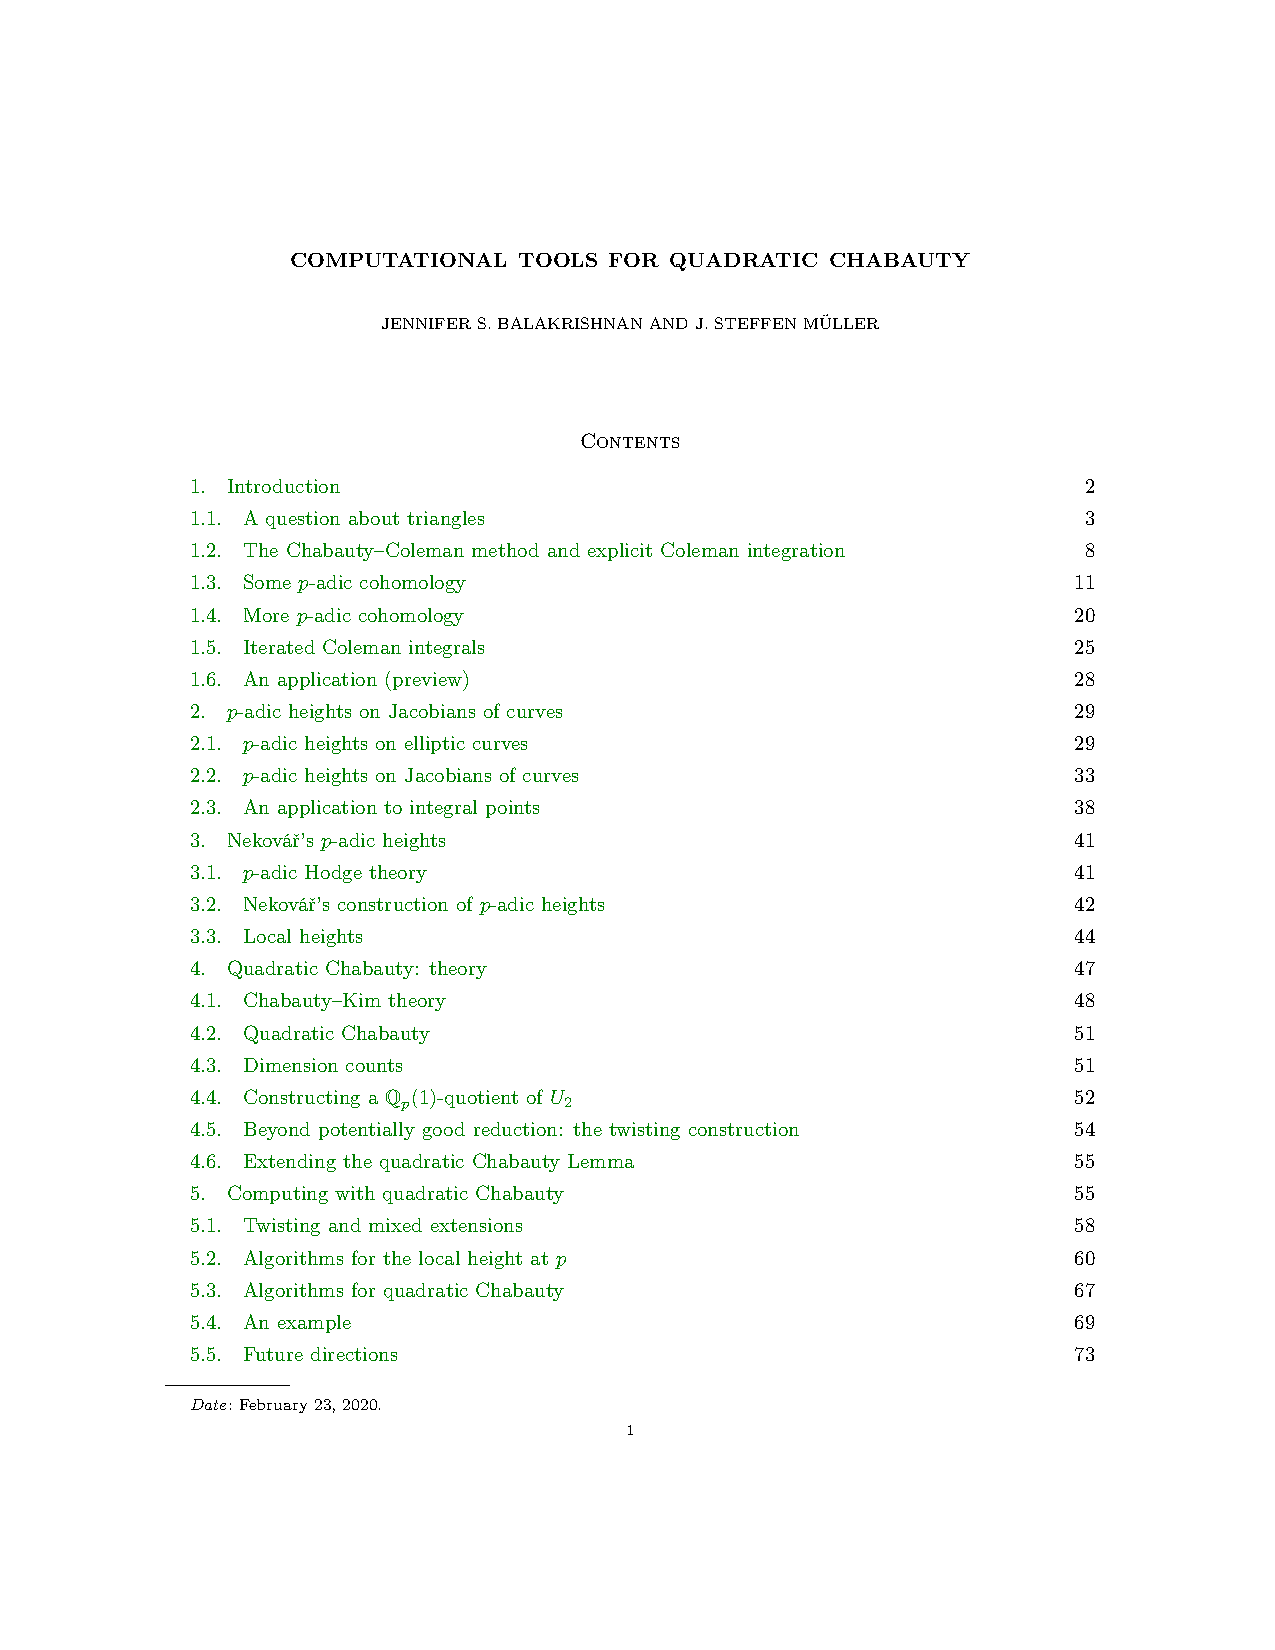
\includepdf[pages=-]{../notes/balakrishnan/2020BalakrishnanMuellerNotes.pdf}

% Edixhoven
\phantomsection
\addtocounter{section}{1}
\addcontentsline{toc}{section}{\protect\numberline{\thesection} Bas Edixhoven: Geometric Quadratic Chabauty}
\phantomsection
\setcounter{subsection}{1}
\addcontentsline{toc}{subsection}{\protect\numberline{\thesubsection}  Course \& Project Outline}
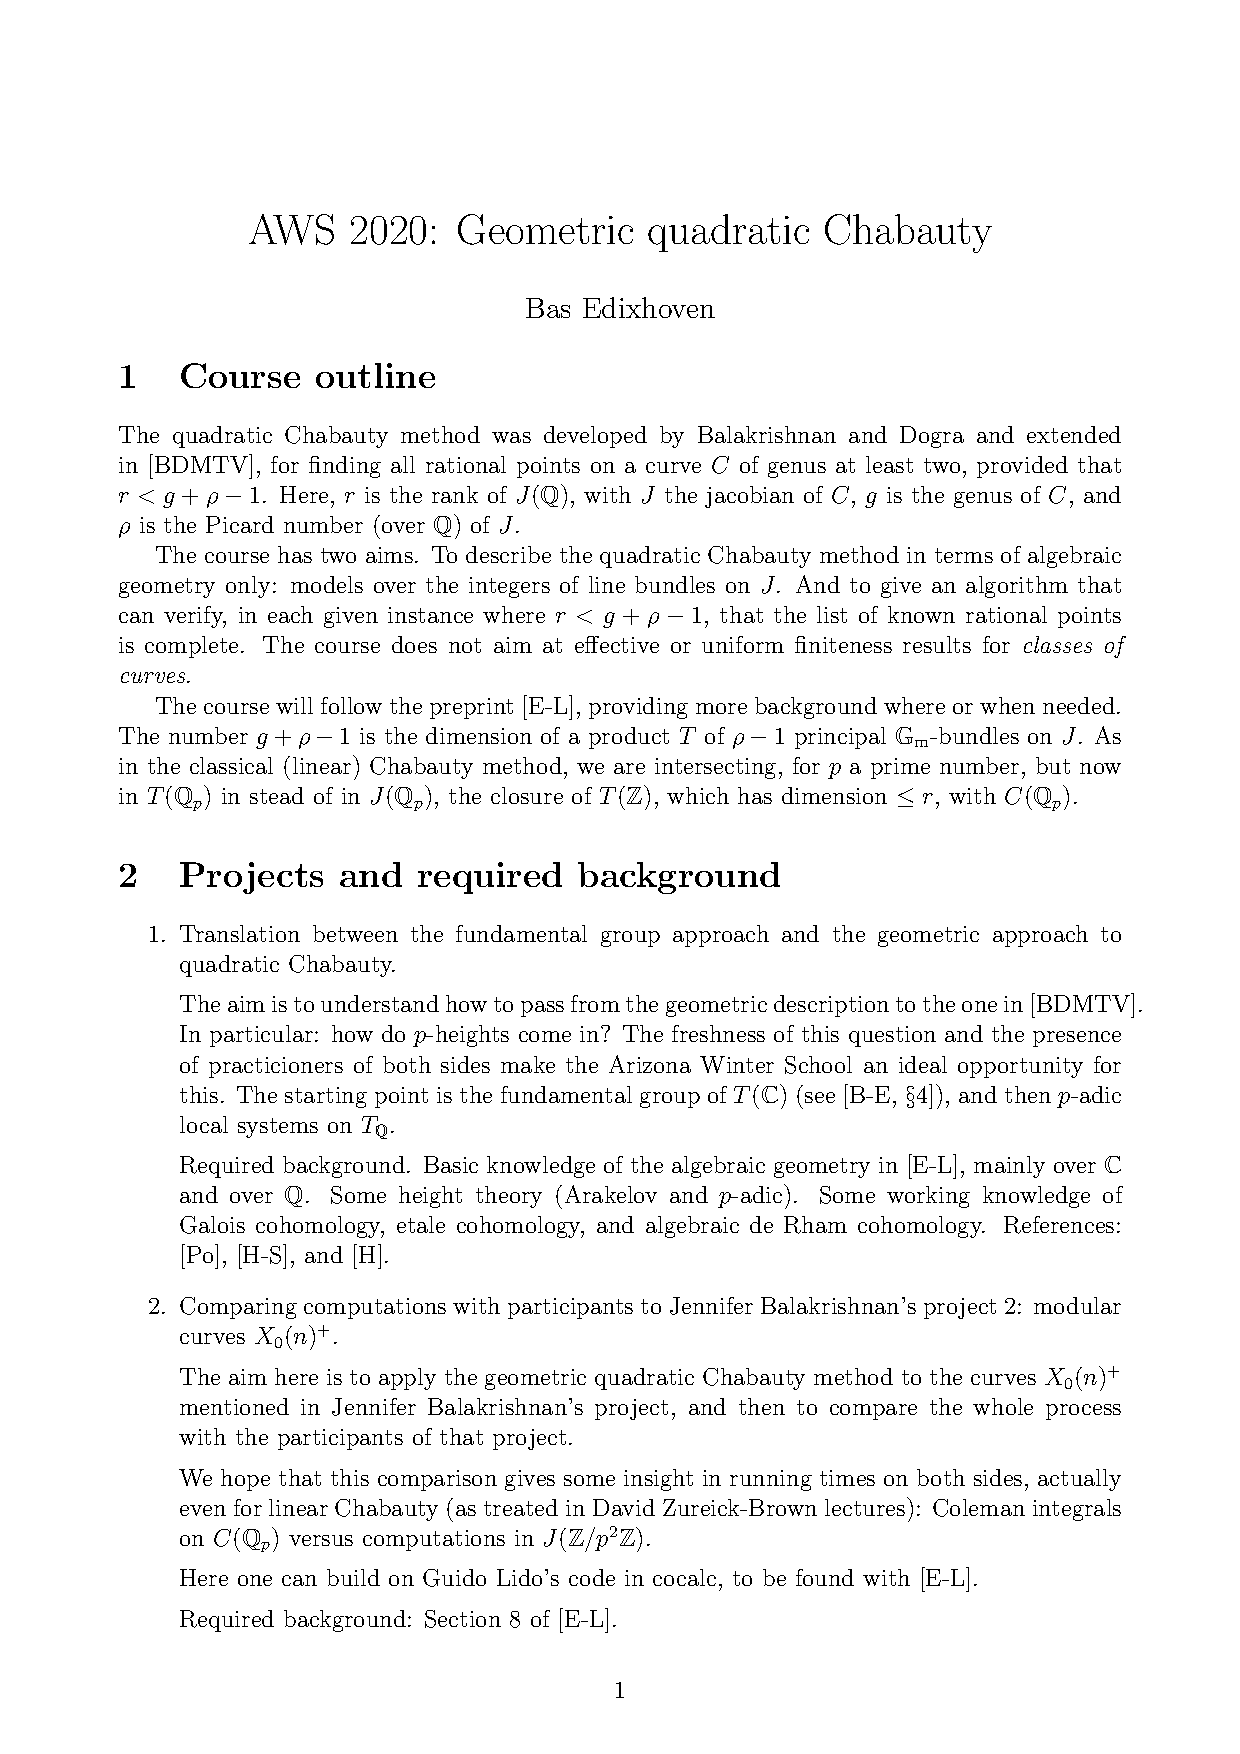
\includepdf[pages=-,scale=1,pagecommand={\thispagestyle{normal}}]{../notes/edixhoven/2020EdixhovenOutline.pdf}
\phantomsection
\addtocounter{subsection}{1}
\addcontentsline{toc}{subsection}{\protect\numberline{\thesubsection} Lecture Notes (Prepreint of Edixhoven and Lido)}
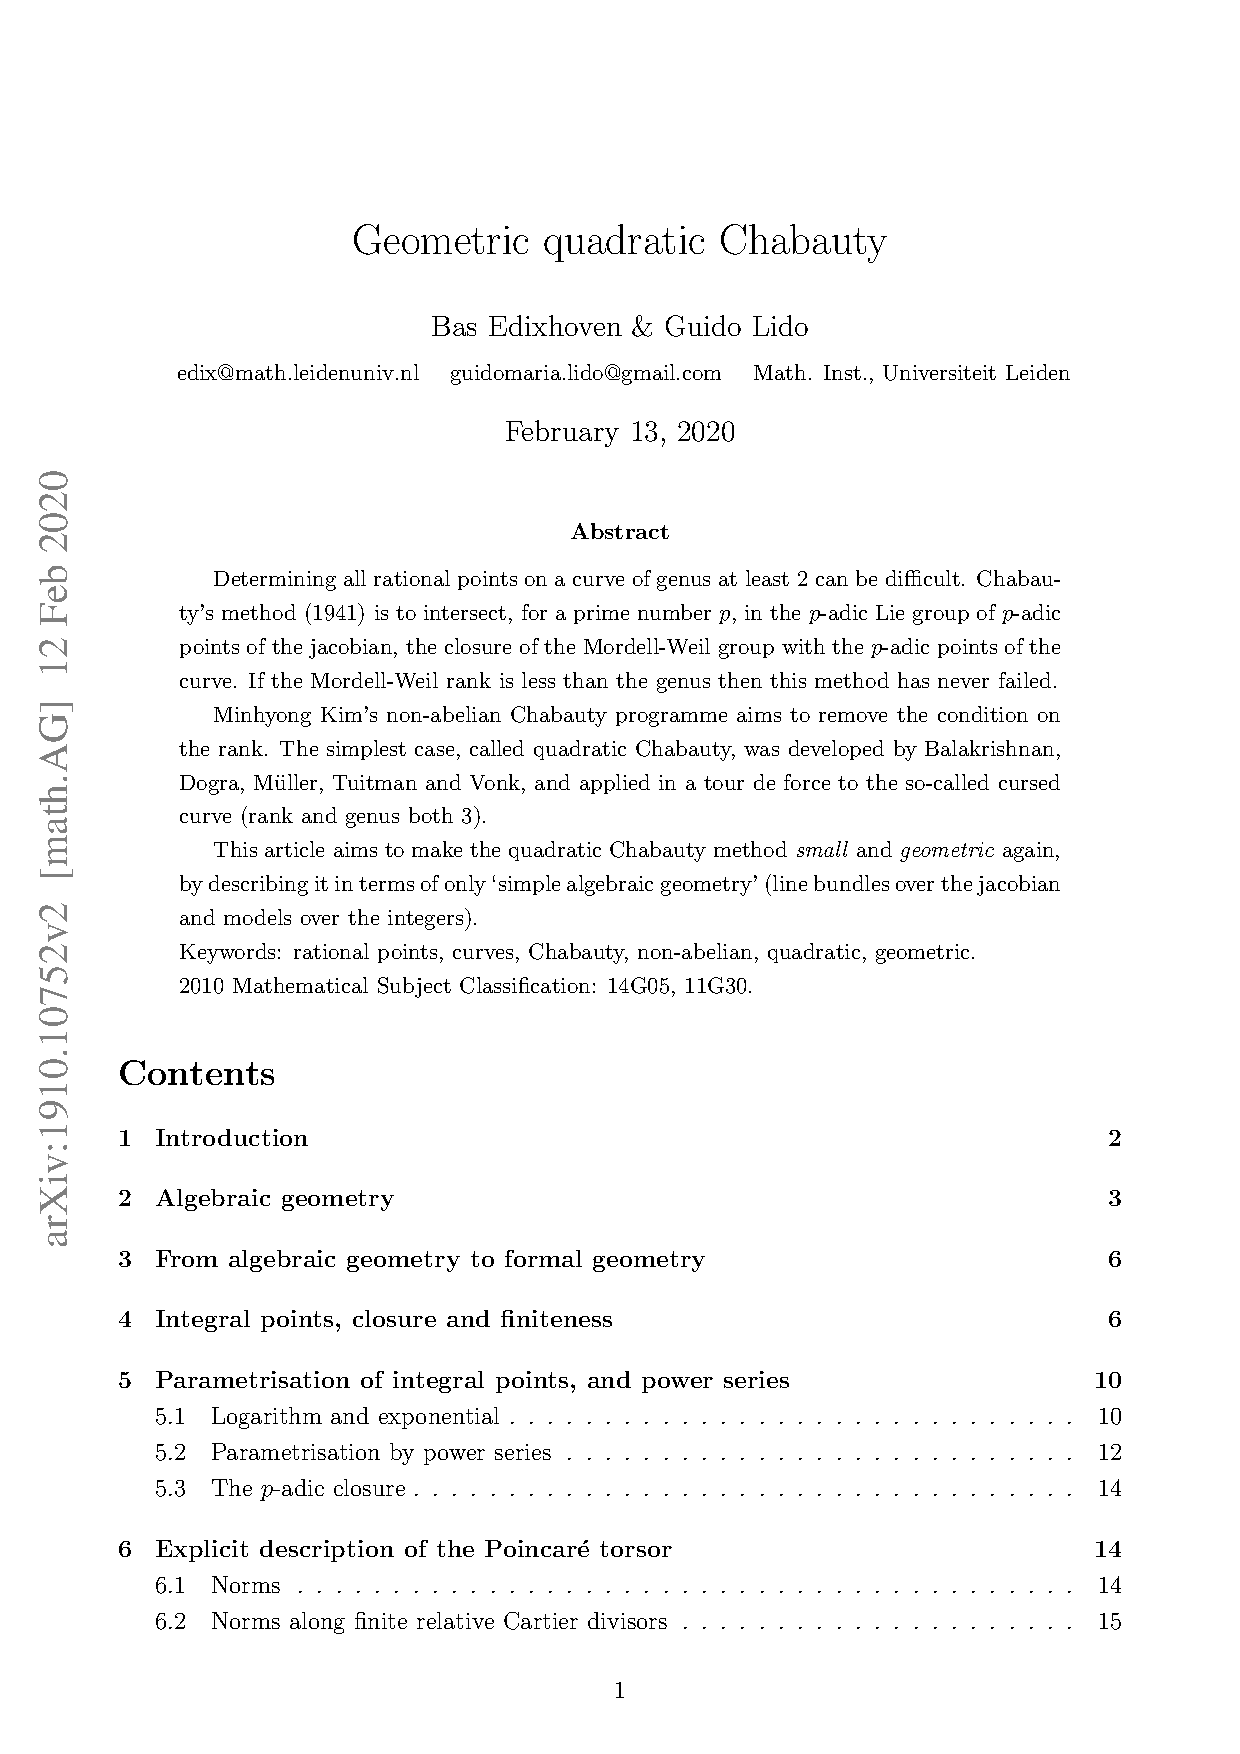
\includepdf[pages=-,scale=1,pagecommand={\thispagestyle{normal}}]{../notes/edixhoven/1910-10752.pdf}
\phantomsection
\addtocounter{subsection}{1}
\addcontentsline{toc}{subsection}{\protect\numberline{\thesubsection} Project Description}
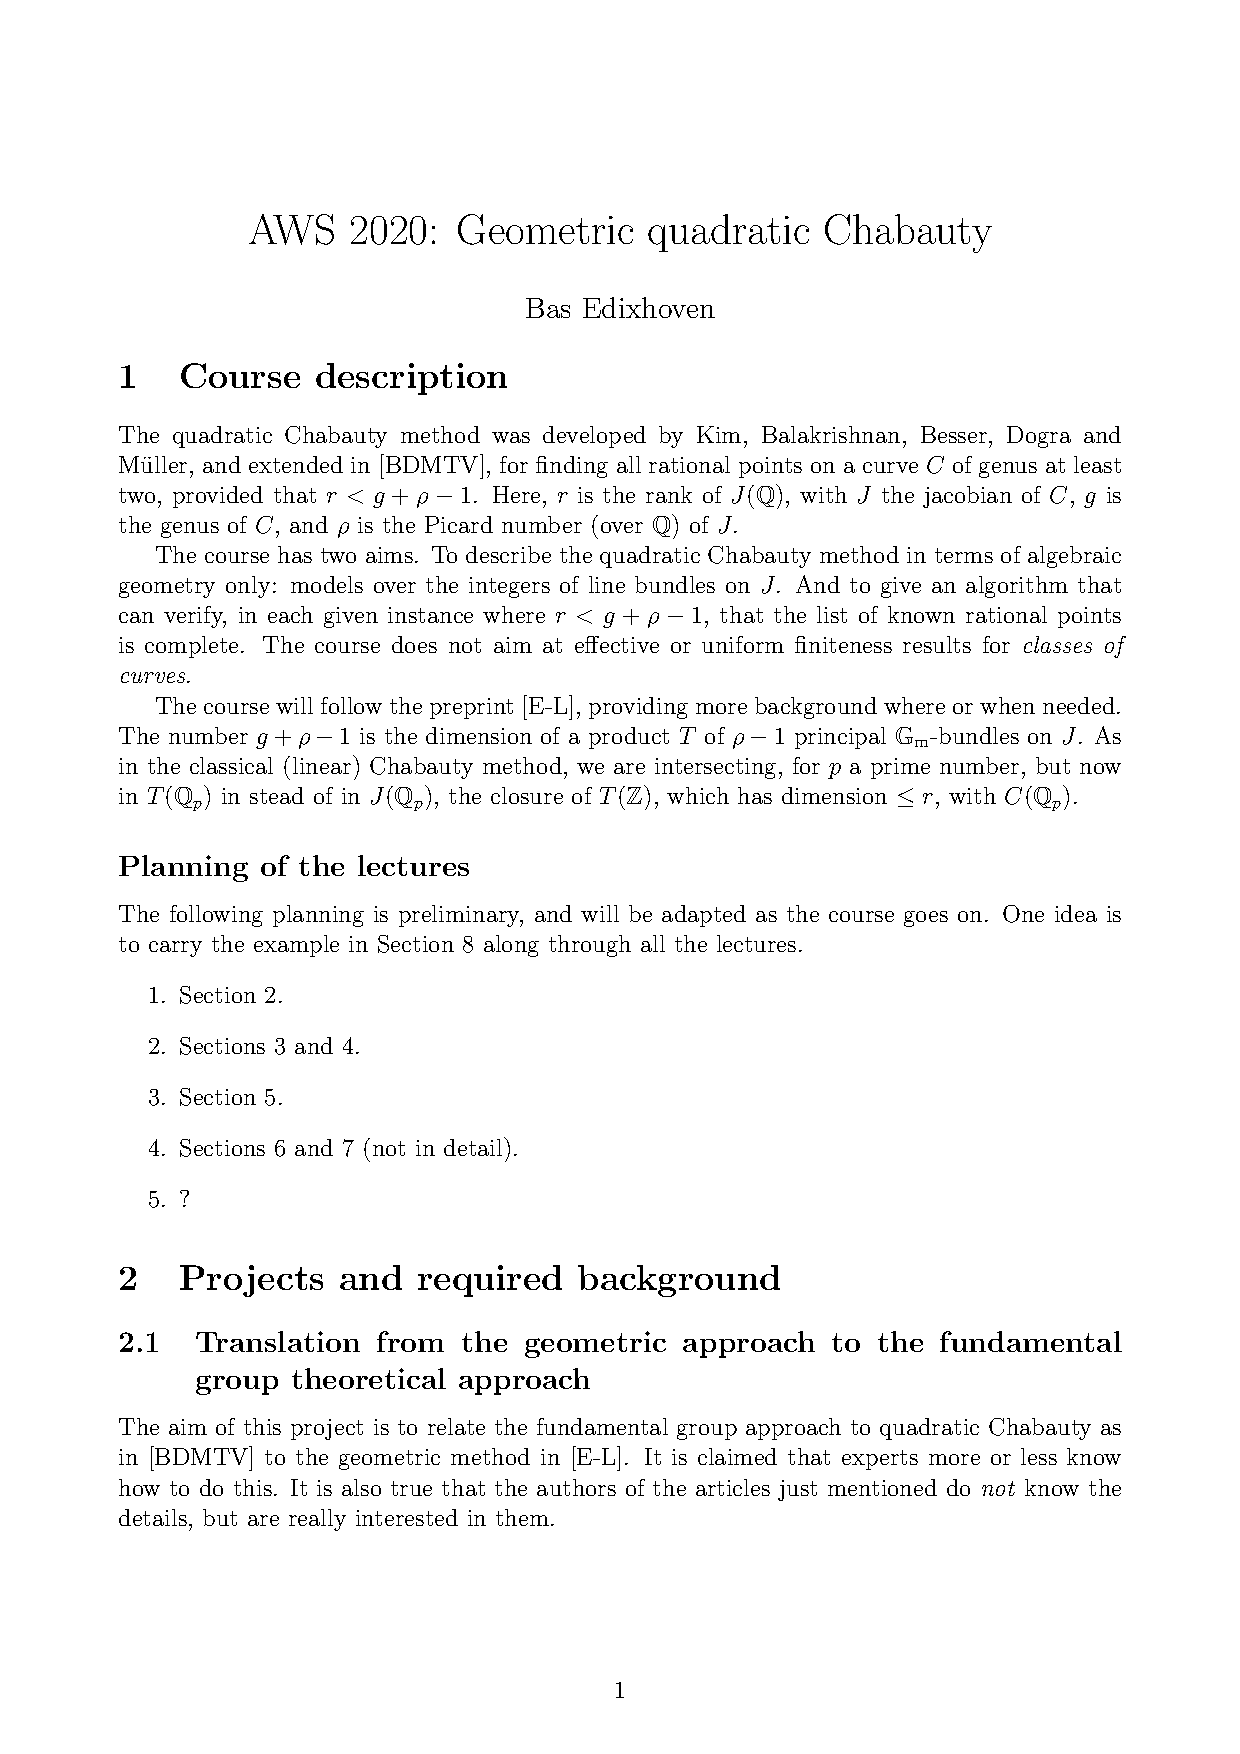
\includepdf[pages=-,scale=1,pagecommand={\thispagestyle{normal}}]{../notes/edixhoven/2020EdixhovenProject.pdf}

% Kim
\phantomsection
\addtocounter{section}{1}
\addcontentsline{toc}{section}{\protect\numberline{\thesection} Minhyong Kim: Foundations of nonabelian Chabauty}
\phantomsection
\setcounter{subsection}{1}
\addcontentsline{toc}{subsection}{\protect\numberline{\thesubsection} Course \& Project Outline}
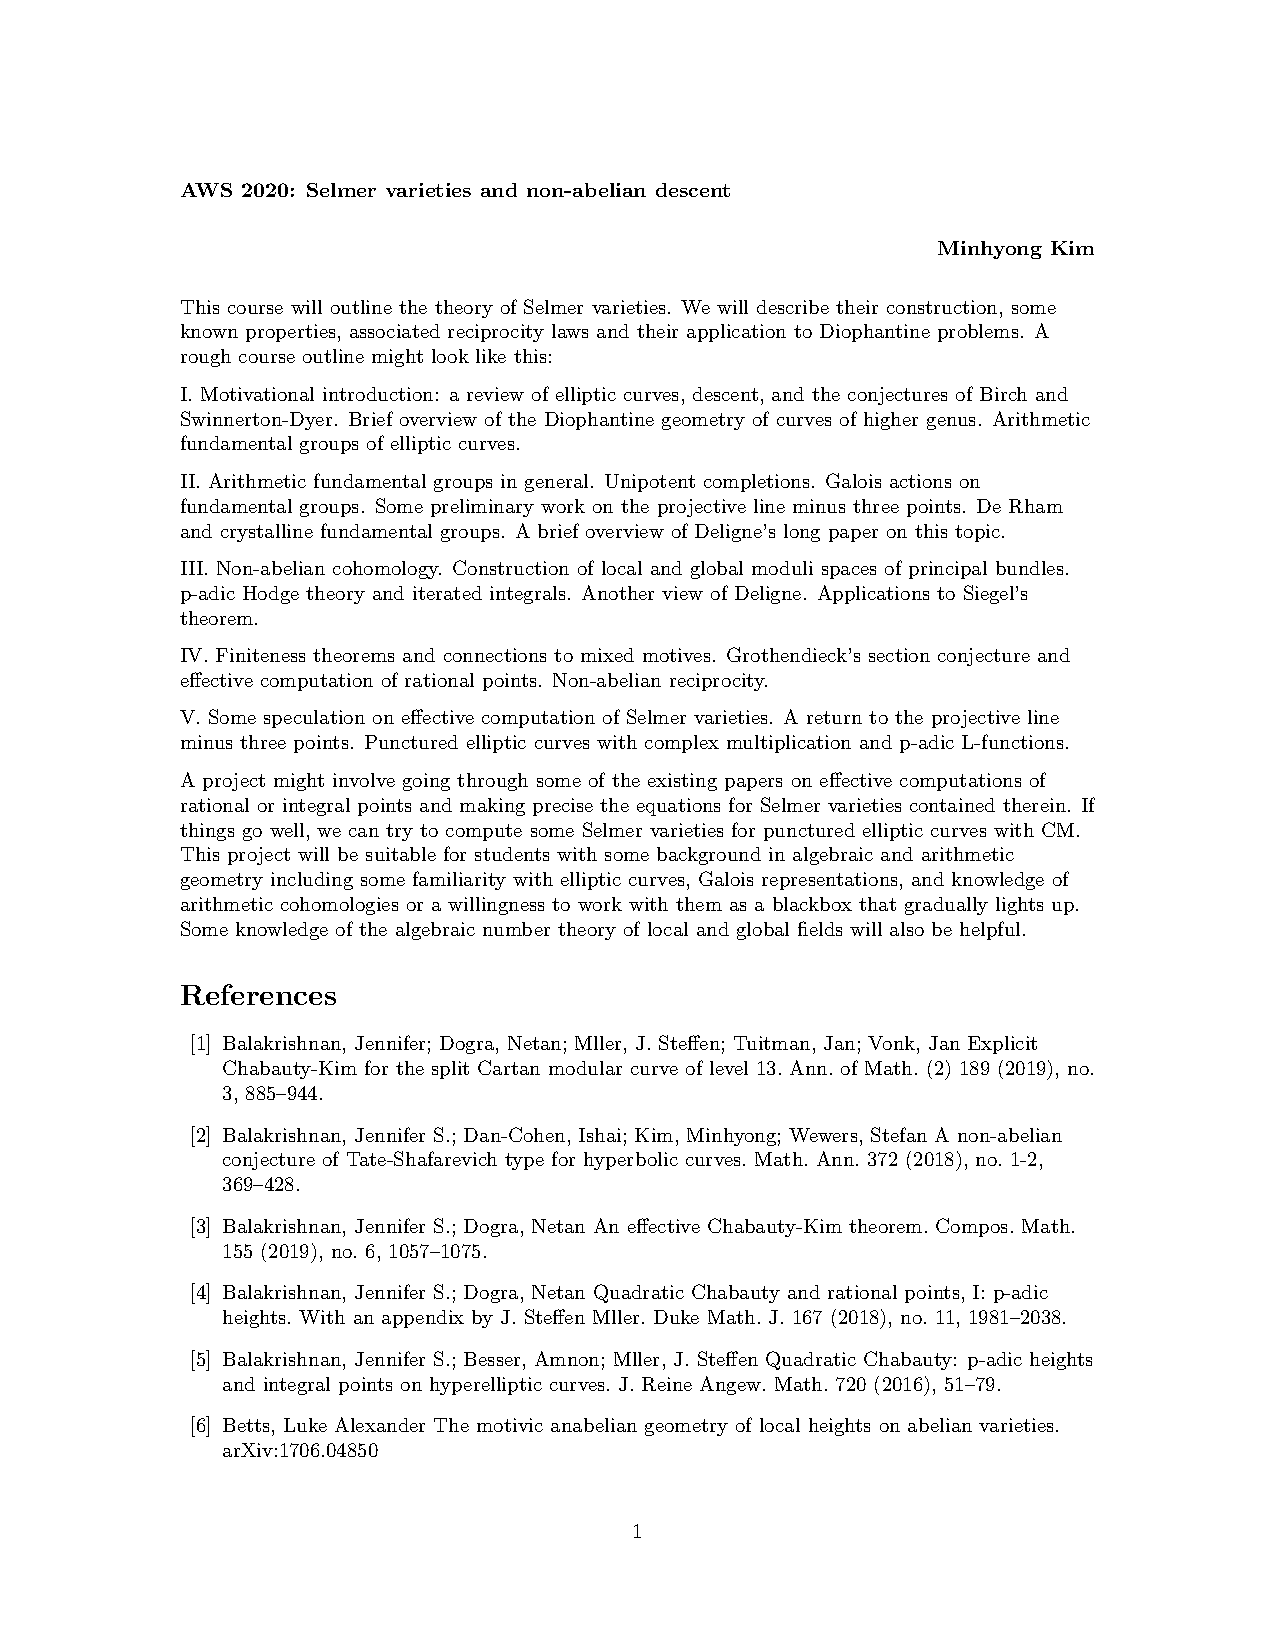
\includepdf[pages=-,scale=1,pagecommand={\thispagestyle{normal}}]{../notes/kim/2020KimOutline.pdf}
\phantomsection
\addtocounter{subsection}{1}
\addcontentsline{toc}{subsection}{\protect\numberline{\thesubsection} Project Description}
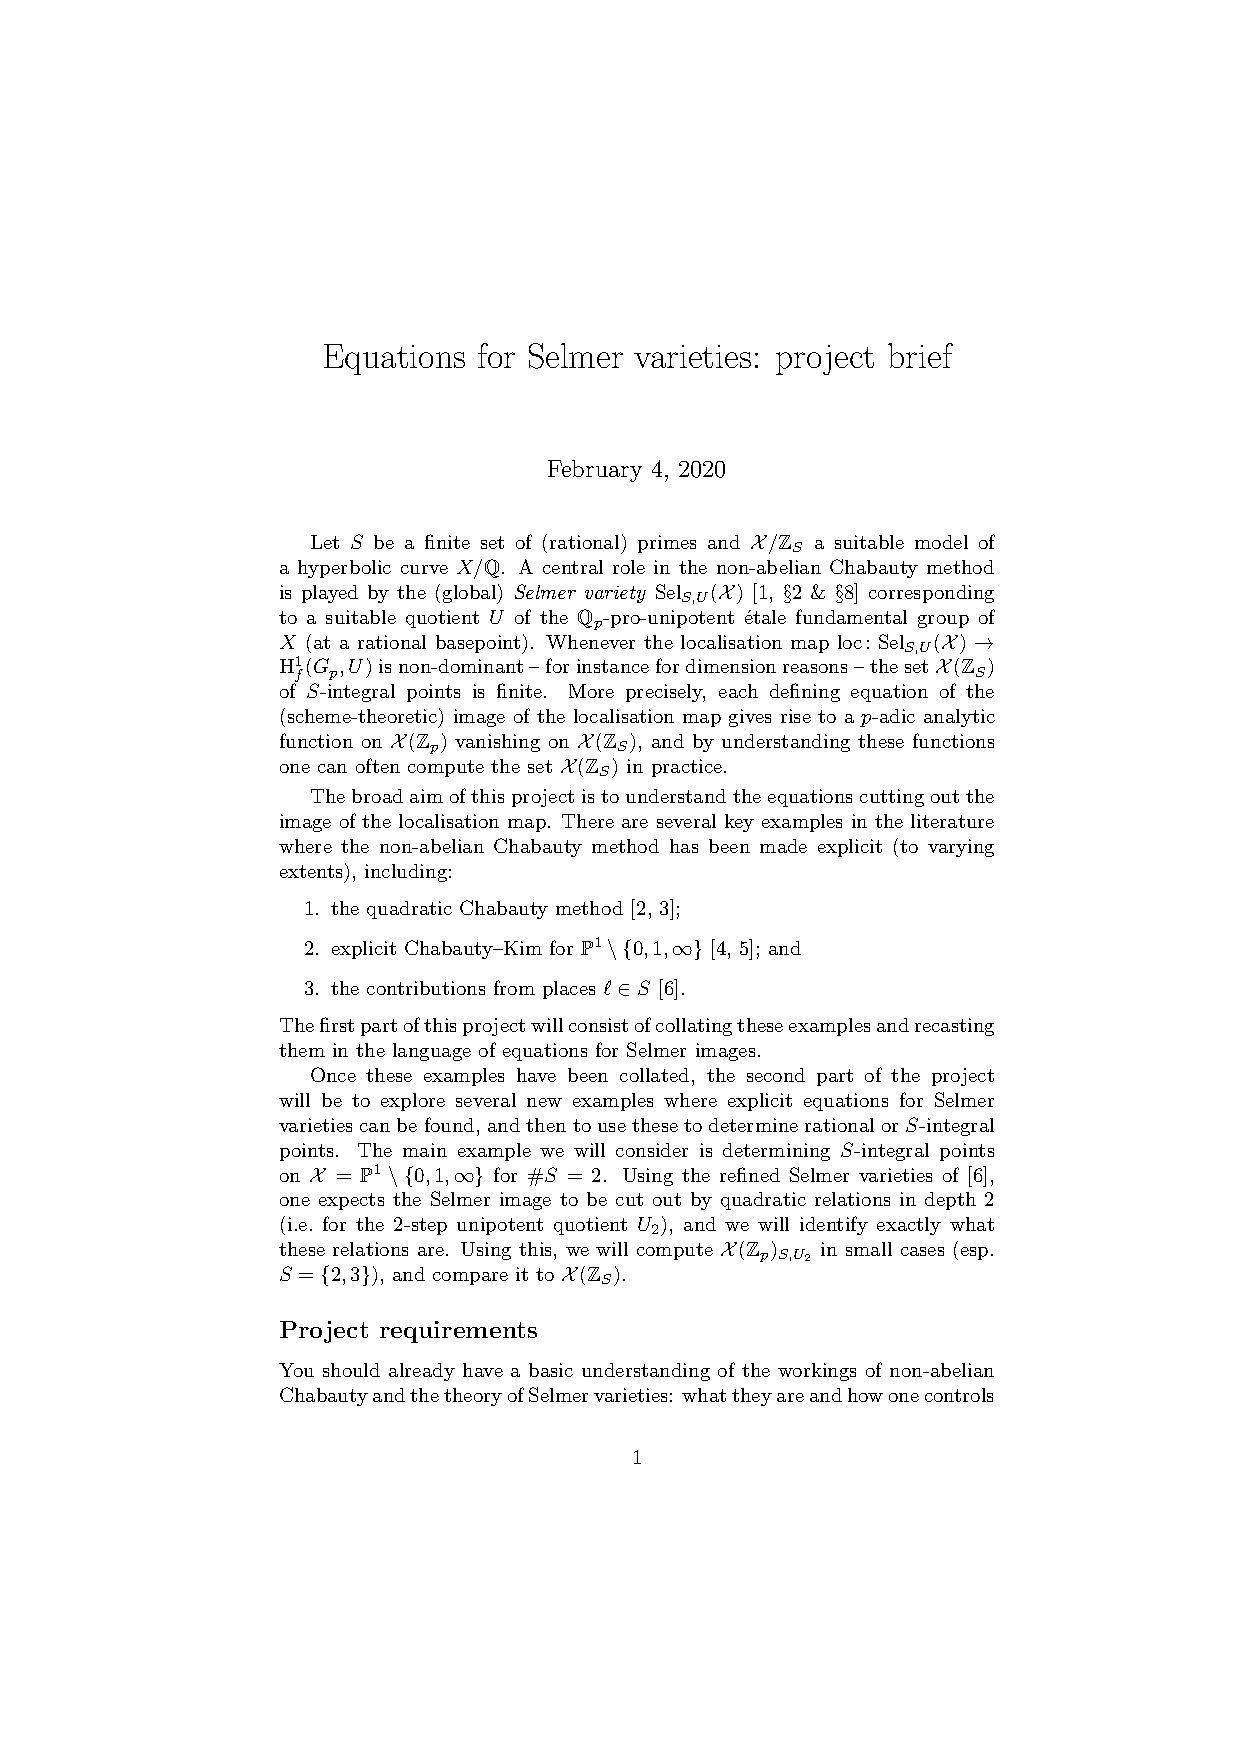
\includepdf[pages=-,scale=1,pagecommand={\thispagestyle{normal}}]{../notes/kim/2020KimProject.pdf}
\phantomsection
\addtocounter{subsection}{1}
\addcontentsline{toc}{subsection}{\protect\numberline{\thesubsection} Lecture 1}

\includepdf[pages=-,scale=1,pagecommand={\thispagestyle{normal}}]{../notes/kim/2020KimNotes1.pdf}
\phantomsection
\addtocounter{subsection}{1}
\addcontentsline{toc}{subsection}{\protect\numberline{\thesubsection} Lecture 2}

\includepdf[pages=-,scale=1,pagecommand={\thispagestyle{normal}}]{../notes/kim/2020KimNotes2.pdf}
\phantomsection
\addtocounter{subsection}{1}
\addcontentsline{toc}{subsection}{\protect\numberline{\thesubsection} Lecture 3}

\includepdf[pages=-,scale=1,pagecommand={\thispagestyle{normal}}]{../notes/kim/2020KimNotes3.pdf}
\phantomsection
\addtocounter{subsection}{1}
\addcontentsline{toc}{subsection}{\protect\numberline{\thesubsection} Lecture 4}
\includepdf[pages=-,scale=1,pagecommand={\thispagestyle{normal}}]{../notes/kim/2020KimNotes4.pdf}

% Zureick-Brown
\phantomsection
\addtocounter{section}{1}
\addcontentsline{toc}{section}{\protect\numberline{\thesection} David Zureick-Brown: Classical Chabauty}
\phantomsection
\setcounter{subsection}{1}
\addcontentsline{toc}{subsection}{\protect\numberline{\thesubsection} Course \& Project Outline}
\includepdf[pages=-,scale=1,pagecommand={\thispagestyle{normal}}]{../notes/zb/2020ZureickBrownOutline.pdf}
\phantomsection
\addtocounter{subsection}{1}
\addcontentsline{toc}{subsection}{\protect\numberline{\thesubsection} Lecture Notes}
\includepdf[pages=-,scale=1,pagecommand={\thispagestyle{normal}}]{../notes/zb/2020ZureickBrownNotes.pdf}
\phantomsection
\addtocounter{subsection}{1}
\addcontentsline{toc}{subsection}{\protect\numberline{\thesubsection} Project Description}
\includepdf[pages=-,scale=1,pagecommand={\thispagestyle{normal}}]{../notes/zb/2020ZureickBrownProjectNotes.pdf}

% Problem Groups
\phantomsection
\addtocounter{section}{1}
\addcontentsline{toc}{section}{\protect\numberline{\thesection} Problem Sessions}
\phantomsection
\setcounter{subsection}{1}
\addcontentsline{toc}{subsection}{\protect\numberline{\thesubsection} Isabel Vogt: Arithmetic of low-genus curves (abridged, no hints)}
\includepdf[pages=-,scale=1,pagecommand={\thispagestyle{normal}}]{../notes/problem_groups/PS2_hintfree.pdf}
\phantomsection
\addtocounter{subsection}{1}
\addcontentsline{toc}{subsection}{\protect\numberline{\thesubsection} Isabel Vogt: Arithmetic of low-genus curves (extended)}
\includepdf[pages=-,scale=1,pagecommand={\thispagestyle{normal}}]{../notes/problem_groups/PS2.pdf}
\phantomsection
\addtocounter{subsection}{1}
\addcontentsline{toc}{subsection}{\protect\numberline{\thesubsection} Daniel Hast: Fundamental groups of curves}
\includepdf[pages=-,scale=1,pagecommand={\thispagestyle{normal}}]{../notes/problem_groups/2020HastProblems.pdf}
\phantomsection
\addtocounter{subsection}{1}
\addcontentsline{toc}{subsection}{\protect\numberline{\thesubsection} Evan Warner: $p$-adic geometry}
\includepdf[pages=-,scale=1,pagecommand={\thispagestyle{normal}}]{../notes/problem_groups/2020WarnerProblems.pdf}
}


% -------------------
% Bibliography
% -------------------
\newpage
\nocite{*}
\printbibliography

\end{document}